\documentclass[11pt,oneside]{book}
\usepackage{fontspec}
\setmainfont{Noto Serif}
\setsansfont{Noto Sans}
\setmonofont{Noto Sans Mono}
\newfontfamily\proseunicodefont{DejaVu Serif}
\usepackage[margin=1in]{geometry}
\usepackage{microtype}
\usepackage{amsmath,amssymb,amsthm,mathtools,bm}
\usepackage{graphicx}
\usepackage{xcolor}
\usepackage{booktabs}
\usepackage{array}
\usepackage{longtable}
\usepackage{enumitem}
\usepackage{float}
\usepackage{caption}
\usepackage{hyperref}
\usepackage{fancyhdr}
\usepackage{tikz}
\usetikzlibrary{arrows.meta,positioning,calc,decorations.pathmorphing}

\hypersetup{
  colorlinks=true,
  linkcolor=blue!50!black,
  urlcolor=blue!50!black,
  citecolor=blue!50!black
}

\setlength{\parskip}{0.5em}
\setlength{\parindent}{0pt}
\setlist[itemize]{topsep=0.25em,itemsep=0.2em}
\setlist[enumerate]{topsep=0.25em,itemsep=0.2em}
\setlength{\headheight}{40pt}
\numberwithin{equation}{chapter}

\newtheorem{theorem}{Теорема}[chapter]
\newtheorem{proposition}[theorem]{Утверждение}
\newtheorem{lemma}[theorem]{Лемма}
\newtheorem{corollary}[theorem]{Следствие}
\theoremstyle{definition}
\newtheorem{definition}[theorem]{Определение}
\newtheorem{example}[theorem]{Пример}
\theoremstyle{remark}
\newtheorem{remark}[theorem]{Замечание}

\providecommand{\ket}[1]{\left\lvert#1\right\rangle}
\providecommand{\bra}[1]{\left\langle#1\right\rvert}
\providecommand{\braket}[2]{\left\langle#1\,\middle|\,#2\right\rangle}
\providecommand{\expect}[1]{\left\langle#1\right\rangle}
\newcommand{\lectureoverview}[1]{\paragraph{Обзор.} #1}

\makeatletter
\newcommand{\course@headerfont}{\normalfont\small\itshape}
\newcommand{\course@pagefont}{\normalfont\small}
\newcommand{\course@headerraise}{14pt}
\newlength{\course@headerboxheight}
\setlength{\course@headerboxheight}{\dimexpr\headheight-\course@headerraise-9pt\relax}
\newcommand{\course@leftheadbox}[1]{%
  \raisebox{\course@headerraise}{%
    \parbox[t][\course@headerboxheight][t]{0.82\textwidth}{%
      \raggedright\course@headerfont\strut\MakeUppercase{#1}\strut%
    }%
  }%
}
\newcommand{\course@rightheadbox}[1]{%
  \raisebox{\course@headerraise}{%
    \parbox[t][\course@headerboxheight][t]{0.82\textwidth}{%
      \raggedleft\course@headerfont\strut\MakeUppercase{#1}\strut%
    }%
  }%
}
\renewcommand{\chaptermark}[1]{\markboth{\MakeUppercase{\chaptername\ \thechapter.\ #1}}{}}
\renewcommand{\sectionmark}[1]{\markright{\MakeUppercase{\thesection\hspace{0.4em}#1}}}
\fancyhf{}
\fancyhead[L]{\course@leftheadbox{\leftmark}}
\fancyhead[R]{\course@pagefont\thepage}
\renewcommand{\headrulewidth}{0.5pt}
\pagestyle{fancy}
\fancypagestyle{plain}{%
  \fancyhf{}
  \fancyhead[L]{\course@leftheadbox{\leftmark}}
  \fancyhead[R]{\course@pagefont\thepage}
  \renewcommand{\headrulewidth}{0.5pt}
}
\makeatother

% Video2Book editorial provenance macros
\newenvironment{classroomqa}{%
  \par\medskip\noindent\begin{minipage}{\linewidth}\small\hrule\medskip
}{%
  \medskip\hrule\end{minipage}\par\medskip
}
\newcommand{\audiencequestion}[1]{\noindent\textbf{Вопрос из аудитории.} #1\par\smallskip}
\newcommand{\lecturerresponse}[1]{\noindent\textbf{Ответ.} #1\par}
\newcommand{\lecturetimestamp}[1]{\footnote{Время в лекции: #1.}}
\newcommand{\lectureframe}[1]{\par\smallskip{\centering\footnotesize\itshape Кадр лекции: #1.\par}}
\newcommand{\editorialnote}[1]{\footnote{Редакторское пояснение: #1}}

\usepackage{polyglossia}
\setdefaultlanguage{russian}
\usepackage{sectsty}
\renewcommand{\contentsname}{Содержание}
\renewcommand{\chaptername}{Глава}
\renewcommand{\figurename}{Рисунок}
\renewcommand{\tablename}{Таблица}
\renewcommand{\proofname}{Доказательство}
\renewcommand{\bibname}{Литература}
\sectionfont{\raggedright}
\subsectionfont{\raggedright}
\makeatletter
\renewcommand{\@pnumwidth}{2.2em}
\renewcommand{\@tocrmarg}{3.2em}
\makeatother
\usepackage{tocloft}
\renewcommand{\cftchapfont}{\small\bfseries}
\renewcommand{\cftchappagefont}{\small\bfseries}
\renewcommand{\cftsecfont}{\small}
\renewcommand{\cftsecpagefont}{\small}
\setlength{\cftsecnumwidth}{3em}
\renewcommand{\cftsubsecfont}{\small}
\renewcommand{\cftsubsecpagefont}{\small}
\setlength{\cftsubsecindent}{4.5em}
\setlength{\cftsubsecnumwidth}{4em}
\emergencystretch=6em
\pdfstringdefDisableCommands{\def\proseunicodefont{}}

\geometry{paperwidth=177.6mm,paperheight=252mm,left=16mm,right=16mm,
 top=18mm,bottom=18mm,includeheadfoot,headheight=28pt,headsep=7mm,footskip=9mm}
\usepackage{scrextend}
\changefontsizes[17pt]{12pt}
\raggedbottom
\renewenvironment{classroomqa}{\par\medskip\begingroup}{\par\endgroup\medskip}
\fancyhf{}
\setlength{\headwidth}{\textwidth}
\fancyhead[L]{\parbox{\textwidth}{\raggedright\fontsize{9}{11}\selectfont\nouppercase{\leftmark}}}
\fancyfoot[C]{\small\thepage}
\renewcommand{\headrulewidth}{0.3pt}
\fancypagestyle{plain}{\fancyhf{}\fancyfoot[C]{\small\thepage}\renewcommand{\headrulewidth}{0pt}}

\graphicspath{{../../../generated_course_notes/core/cosmology/2009_winter_legacy_cosmology/figures/}{../../../generated_course_notes/core/cosmology/2009_winter_legacy_cosmology/assets/}}
\begin{document}
\frontmatter
\hypersetup{pageanchor=false}
\begin{titlepage}
\hyphenpenalty=10000\exhyphenpenalty=10000
\thispagestyle{empty}
\begin{tikzpicture}[remember picture,overlay]
  \node[anchor=center,inner sep=0] at (current page.center) {%
    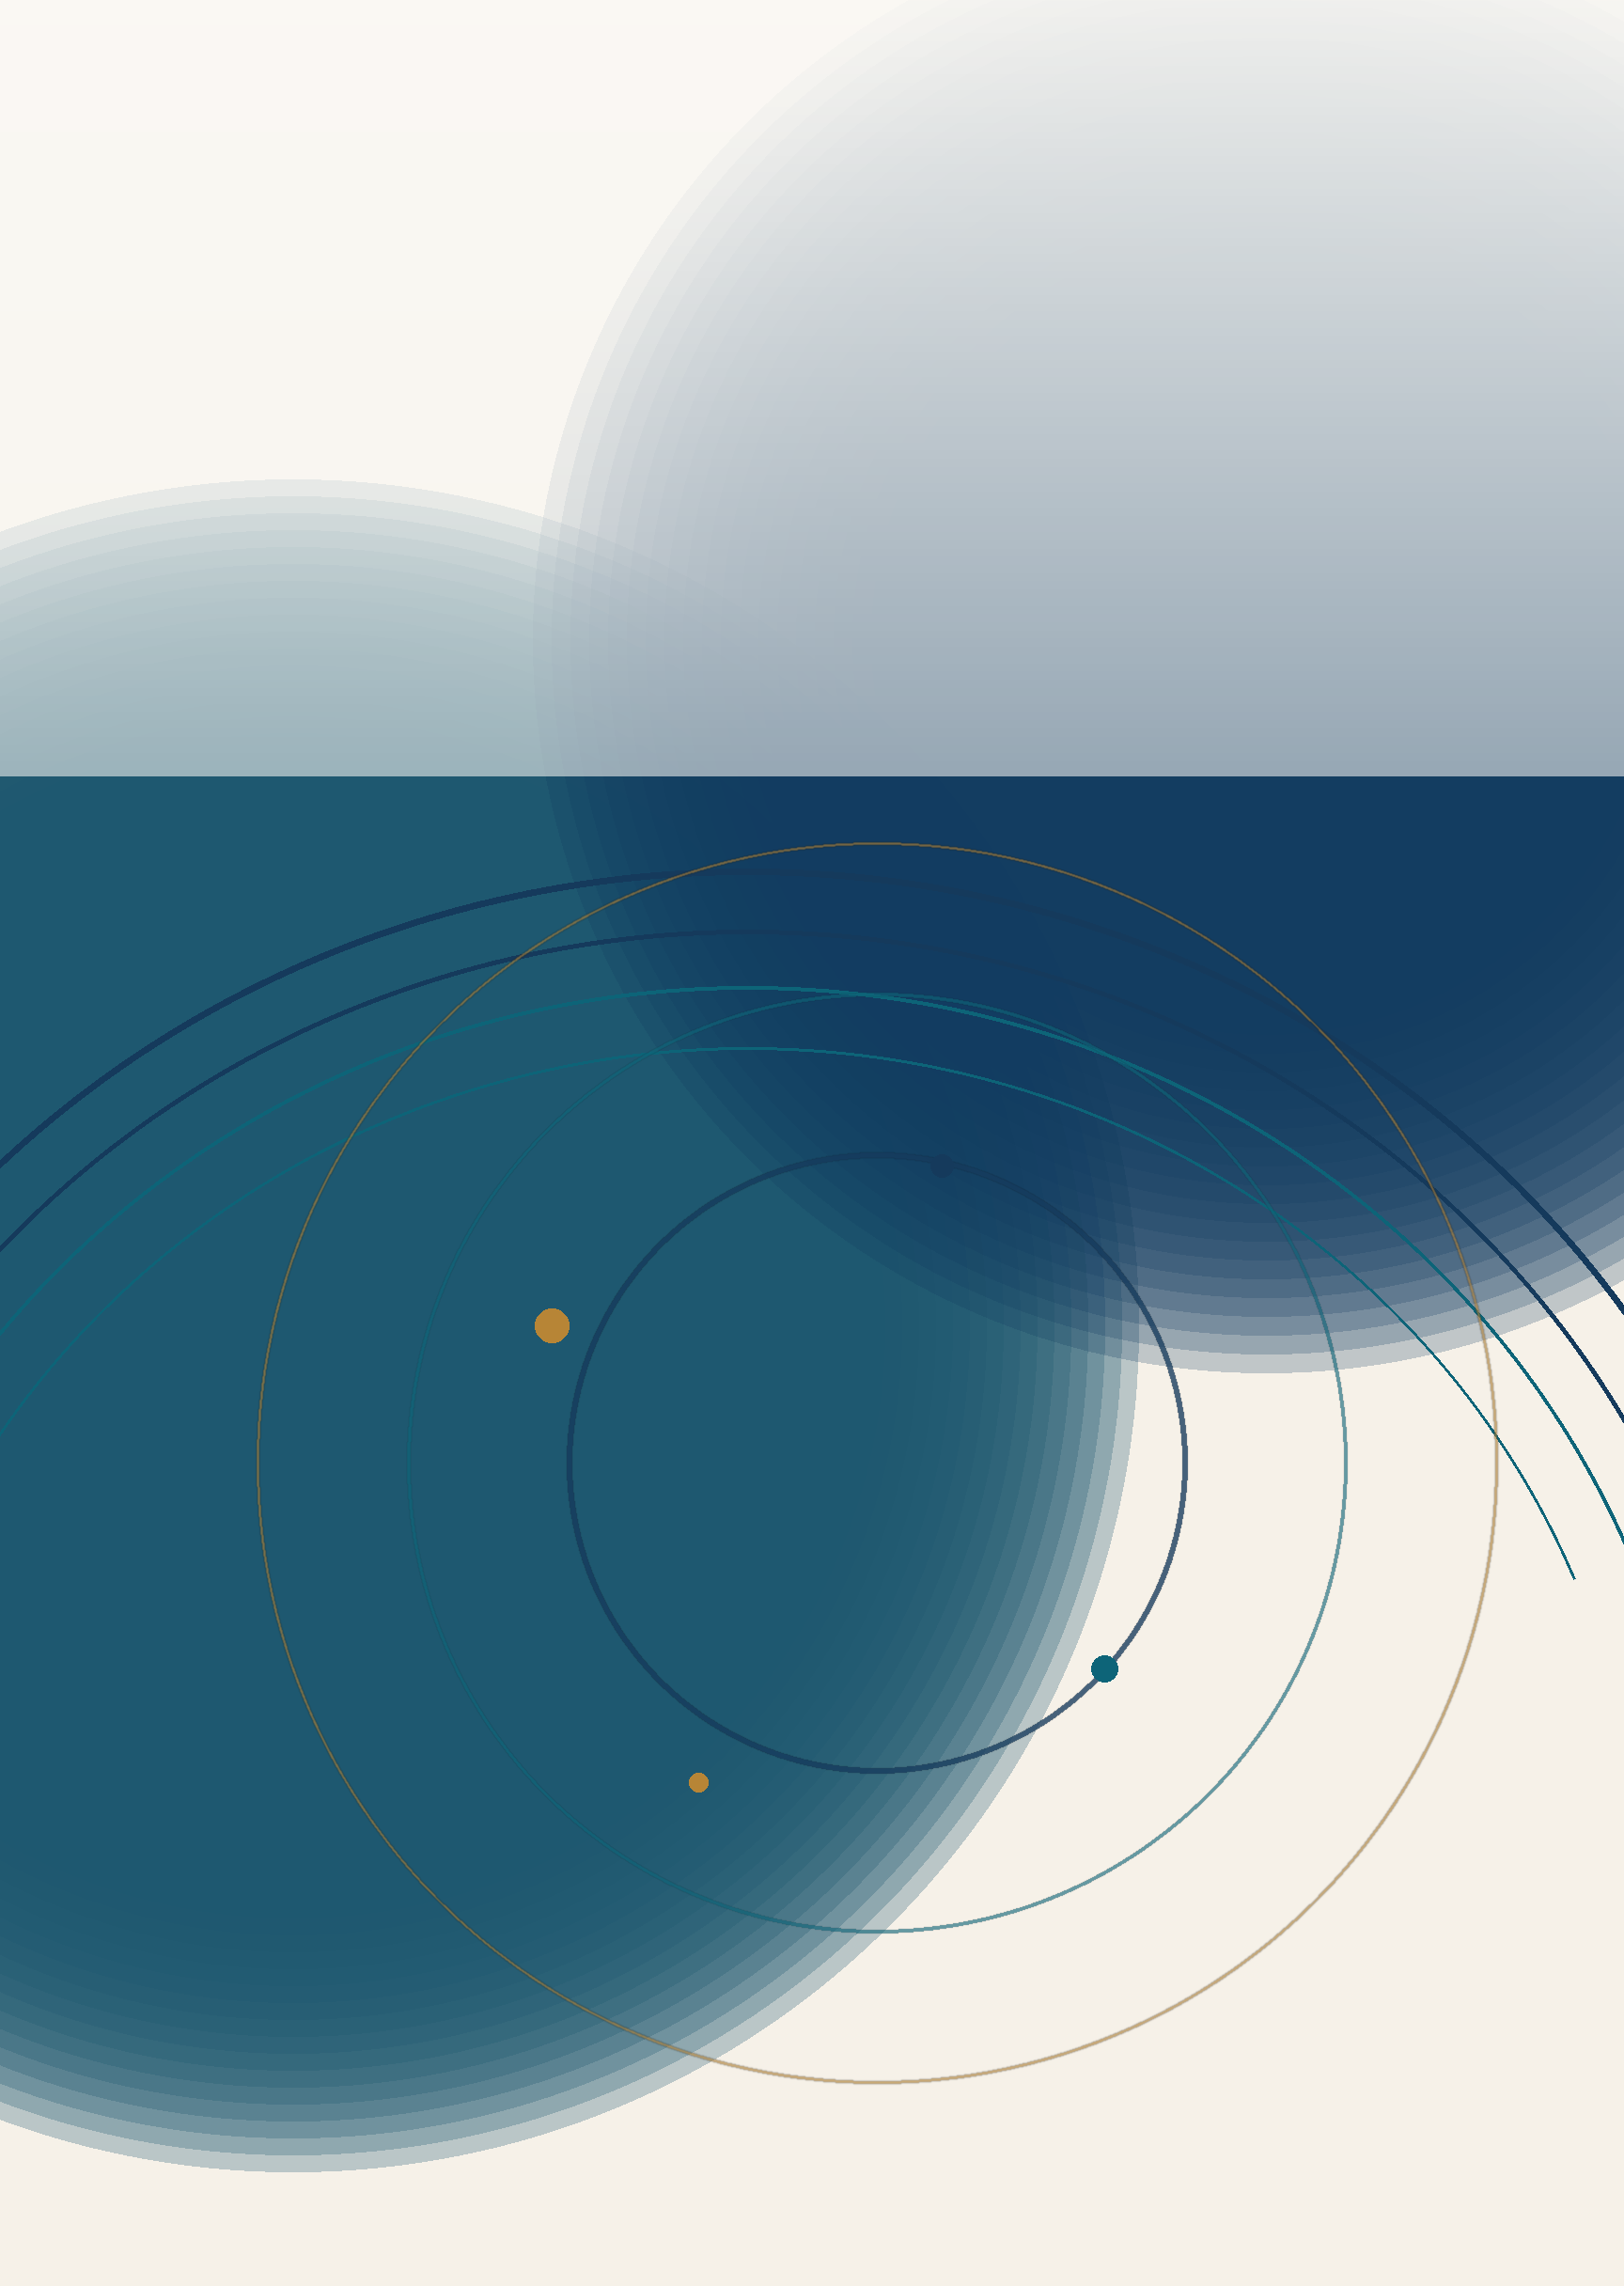
\includegraphics[height=\paperheight,keepaspectratio]{../../../generated_course_notes/core/cosmology/2009_winter_legacy_cosmology/assets/cover-art.png}%
  };
  \node[
    anchor=north west,
    align=left,
    text width=0.78\paperwidth,
    fill=white,
    fill opacity=0.9,
    rounded corners=8pt,
    inner xsep=10pt,
    inner ysep=8pt
  ] at ([xshift=0.08\paperwidth,yshift=-0.06\paperheight]current page.north west) {%
    {\fontsize{30}{33}\selectfont\bfseries\color{black!88} Космология\\[0.85em]}
    {\large\color{black!72} Русское издание / зима 2009, предыдущий курс космологии}
  };
  \node[
    anchor=south west,
    align=left,
    text width=0.68\paperwidth,
    fill=white,
    fill opacity=0.82,
    text opacity=1,
    rounded corners=6pt,
    inner sep=12pt
  ] at ([xshift=0.08\paperwidth,yshift=0.08\paperheight]current page.south west) {%
    {\normalsize\color{black!78} Оригинальные лекции: Leonard Susskind\\[0.35em]}
    {\small\color{black!72} Сопроводительное издание: \href{https://lazying.art}{LazyingArt LLC} / \href{https://github.com/lachlanchen/Video2Book}{Video2Book}}
  };
\end{tikzpicture}
\mbox{}
\end{titlepage}
\hypersetup{pageanchor=true}

\clearpage
\chapter*{Об этих заметках}
Эти независимо отредактированные сопроводительные заметки составлены по лекциям Леонарда Сасскинда. Они были восстановлены по машинным расшифровкам, субтитрам и выбранным кадрам с доской, а затем сверены с доступными исходными материалами. Это не оригинальная рукопись профессора Сасскинда, и он ее не проверял и не одобрял.

Это издание было подготовлено \href{https://lazying.art}{LazyingArt LLC} с использованием рабочего процесса \href{https://github.com/lachlanchen/Video2Book}{Video2Book} с открытым исходным кодом. Машинные расшифровки по-прежнему доступны отдельно и могут содержать ошибки распознавания. Редакторские уточнения и нетривиальные реконструкции отмечены в сносках.
\clearpage
\tableofcontents
\mainmatter
\chapter{Геометрия расширяющейся Вселенной}

Речь идет о расширяющейся Вселенной и ее геометрии. Цель состоит в том, чтобы описать, что значит расширение пространства, прежде чем спрашивать, что вызывает это расширение. Ньютоновская \(F=ma\) космология будет позже, и лишь после этого геометрия и динамика будут объединены в полный формализм Фридмана--Робертсона--Уокера.

\section{Сопутствующие координаты на расширяющейся прямой}

Начнем с простейшего возможного примера: одномерного пространства, а не пространства-времени. Представьте себе бесконечную прямую с равномерно расположенными на ней галактиками. Координата \(x\) пока еще не измеряет физическое расстояние. Она служит меткой для галактик. Можно думать об \(x\) как об имени галактики, и это имя остается связанным с галактикой, даже если вся конфигурация растягивается или сжимается.

Пусть физическое расстояние от галактики с меткой \(x=0\) до галактики с меткой \(x=1\) равно \(a\). Тогда физическое расстояние между любыми двумя галактиками равно
\begin{equation}
d=a\,\Delta x.
\end{equation}
Координатная разность \(\Delta x\) — это лишь разность меток. Множитель \(a\) переводит эту разность меток в действительное расстояние, измеряемое метровыми стержнями.

Теперь представьте эту прямую как упругую нить, которую растягивают. Метки остаются при галактиках, но расстояние между соседними галактиками меняется со временем. То же соотношение принимает вид
\begin{equation}
d(t)=a(t)\,\Delta x.
\end{equation}
На этом этапе однородность означает просто, что соседние галактики повсюду расположены на одинаковом расстоянии друг от друга, хотя это общее расстояние может меняться со временем.

\section{Закон Хаббла и отсутствие центра}

Чтобы найти относительную скорость двух фиксированных галактик, будем рассматривать одну и ту же пару, так что \(\Delta x\) не меняется со временем. Дифференцируя, получаем
\begin{align}
\dot d &= \dot a\,\Delta x \\
       &= \frac{\dot a}{a}\,a\,\Delta x \\
       &= \frac{\dot a}{a}\,d.
\end{align}
Если определить
\begin{equation}
H(t)\equiv \frac{\dot a}{a},
\end{equation}
то
\begin{equation}
\dot d = H(t)\,d.
\end{equation}
Это и есть закон Хаббла.

Историческое выражение ``постоянная Хаббла'' вводит в заблуждение. Эта величина постоянна в пространстве, а не во времени. В данный момент она одинакова для каждой галактики, но, вообще говоря, меняется по мере эволюции Вселенной. Ее правильнее рассматривать как параметр Хаббла.

Этот закон говорит, что более далекие галактики удаляются быстрее. Он не выделяет никакого центра. Ничто в этом рассуждении не выделяет \(x=0\) или любую другую точку. Каждый наблюдатель видит одно и то же правило. Следовательно, расширяющаяся Вселенная в этой модели не является взрывом из одного выделенного места.

Красное смещение появляется сразу. Если две галактики обмениваются световыми сигналами, удаляясь друг от друга, принятый свет смещается в красную сторону. Чем больше скорость удаления, тем больше красное смещение. Поэтому спектральные линии сообщают нам о скоростях удаления. Расстояния измерять труднее, и ранние оценки Хаббла были грубыми. Его первый график был не идеальной прямой, а разрозненным набором точек с большими неопределенностями. И все же геометрический принцип пережил этот шум: скорость удаления пропорциональна расстоянию.

\begin{classroomqa}
\audiencequestion{Если галактики достаточно далеко друг от друга, следует ли из закона Хаббла, что они движутся быстрее скорости света?}\lecturetimestamp{00:20:23}
\lecturerresponse{Да, в этом смысле удаления — да. То, что вы говорите, верно. Мы к этому обязательно вернемся. Это одна из самых важных вещей.}
\end{classroomqa}

\section{Более высокие размерности, изотропия и временная зависимость \(a(t)\)}

При добавлении большего числа пространственных измерений по существу ничего не меняется. В двух измерениях представьте квадратную решетку галактик, помеченных координатами \((x,y)\), а в трех измерениях — координатами \((x,y,z)\). Эти координаты снова являются сопутствующими метками. Они движутся вместе с галактиками, а не измеряют непосредственно физическое расстояние.

Почему расстояние в направлении \(x\) должно быть таким же, как расстояние в направлении \(y\)? Ответ дает наблюдение. Если бы галактики в одном направлении систематически располагались плотнее, чем в другом, небо выглядело бы по-разному в разных направлениях. На достаточно больших масштабах этого нет. Эта одинаковость по направлениям и есть изотропия.

В двух измерениях расстояние между двумя галактиками равно
\begin{equation}
d=a\sqrt{(\Delta x)^2+(\Delta y)^2},
\end{equation}
а в трех измерениях
\begin{equation}
d=a\sqrt{(\Delta x)^2+(\Delta y)^2+(\Delta z)^2}.
\end{equation}
Для фиксированной пары галактик координатные разности остаются постоянными, поэтому дифференцирование снова дает
\begin{equation}
\dot d=\frac{\dot a}{a}\,d.
\end{equation}
Закон Хаббла не меняется.

Однородность означает одинаковость от места к месту. Изотропия означает одинаковость от направления к направлению. Ни то ни другое не является точным на малых масштабах. Смотреть сквозь Млечный Путь — не то же самое, что смотреть вне его плоскости, и отдельные галактики на малых расстояниях распределены неравномерно. Но после усреднения по многим галактикам Вселенная на больших масштабах выглядит приблизительно одинаковой везде и во всех направлениях.

\begin{classroomqa}
\audiencequestion{Если скорость пропорциональна расстоянию и расстояние увеличивается, означает ли это, что фиксированная пара галактик обязательно должна удаляться друг от друга с ускорением?}\lecturetimestamp{00:40:22}
\lecturerresponse{Нет. Закон Хаббла говорит, что в данный момент скорость удаления пропорциональна расстоянию. Сам по себе он не говорит, увеличивается или уменьшается со временем скорость одной фиксированной пары. Это зависит от конкретной временной зависимости \(a(t)\). Если \(a(t)\propto t\), соседние галактики расходятся с постоянной скоростью. Если \(a(t)\propto t^2\), скорость удаления фиксированной пары растет со временем. Если \(a(t)\propto \log t\), она уменьшается со временем. Закон \(\dot d=(\dot a/a)d\) всегда верен как функция расстояния, но ускорение и замедление — отдельные вопросы.}
\end{classroomqa}

Долгое время космологи ожидали, что Вселенная должна расширяться с замедлением, поскольку гравитация должна тормозить начальное расширение так же, как она замедляет тело, брошенное вверх. Здесь важно лишь то, что сам по себе закон Хаббла не определяет поведение \(\dot a\) или \(\ddot a\).

\begin{classroomqa}
\audiencequestion{Как задается начальное значение масштабного фактора \(a\)?}\lecturetimestamp{00:46:18}
\lecturerresponse{Его общая нормировка произвольна. Физически важно не численное значение \(a\) само по себе, а то, как оно меняется. Если определить другой масштабный фактор \(b=3a\), то \(\dot b/b=\dot a/a\). Умножение \(a\) на постоянный множитель меняет соглашения или единицы измерения, но не параметр Хаббла.}
\end{classroomqa}

\section{От пространственной метрики к метрике пространства-времени}

Теперь заменим \(\Delta x\) на \(dx\). Физическое расстояние между соседними точками равно
\begin{equation}
ds=a\,dx,
\end{equation}
так что
\begin{equation}
ds^2=a^2\,dx^2.
\end{equation}
Это пространственная метрика в одном измерении. Коэффициент при \(dx^2\) равен
\begin{equation}
g_{xx}=a^2.
\end{equation}
Следовательно, расширяющуюся Вселенную можно описать, сказав, что пространственная часть метрики зависит от времени.

Чтобы перейти от пространства к пространству-времени, используем релятивистский интервал. В одном пространственном измерении,
\begin{equation}
d\tau^2=dt^2-a^2(t)\,dx^2.
\end{equation}
Для сопутствующего наблюдателя \(dx=0\), так что \(d\tau=dt\). Обычное космическое время — это собственное время, измеряемое часами, движущимися вместе с галактиками.

Рисунок на доске на этом этапе полезен, потому что он объединяет сопутствующие мировые линии, элемент линии и обозначения метрики.
\begin{figure}[H]
\centering
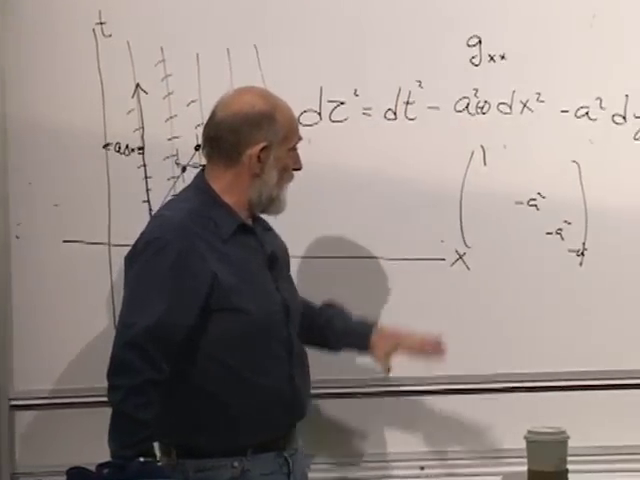
\includegraphics[width=0.82\textwidth]{lecture_01_figure_02.png}
\caption{Сопутствующие мировые линии в расширяющейся одномерной Вселенной вместе с соответствующим интервалом пространства-времени.}
\end{figure}

В трех пространственных измерениях тот же образец дает осторожное обобщение\footnote{Доска частично закрыта в районе 00:56:38--00:58:51. Эта трехмерная форма следует из устного перехода от одного пространственного измерения к трем вместе с видимой на доске диагональной структурой.}
\begin{equation}
d\tau^2=dt^2-a^2(t)\bigl(dx^2+dy^2+dz^2\bigr),
\end{equation}
с диагональной метрикой
\begin{equation}
g_{\mu\nu}=\mathrm{diag}\bigl(1,-a^2,-a^2,-a^2\bigr).
\end{equation}
Внедиагональные члены обращаются в нуль,
\begin{equation}
g_{tx}=g_{ty}=g_{tz}=0.
\end{equation}

Однородность означает, что коэффициенты метрики могут зависеть от времени, но не от пространственного положения. Изотропия означает, что все три пространственных направления входят одинаковым образом.

\begin{classroomqa}
\audiencequestion{Разве не следует думать об \(dx\) как о расстоянии?}\lecturetimestamp{01:01:18}
\lecturerresponse{Нет. \(dx\) — это не расстояние. \(a\,dx\) — это расстояние. \(dx\) — всего лишь интервал меток. Полезно думать об этом так: представьте, что в некоторый момент кто-то проводит координатную сетку через галактики, а затем требует, чтобы она следовала за ними. Координатное разделение по построению остается фиксированным, тогда как физическое расстояние меняется. Можно было бы поместить единицы длины в \(x\), а не в \(a\); это вопрос соглашения. Важно произведение \(a\,dx\).}
\end{classroomqa}

\begin{classroomqa}
\audiencequestion{Коэффициент при \(dt^2\) в метрике равен \(1\). Это тоже просто вопрос соглашения?}\lecturetimestamp{01:03:24}
\lecturerresponse{Да. Само по себе здесь никакой физики нет. Если бы коэффициент зависел только от времени, можно было бы изменить временную переменную так, чтобы он стал просто \(dt^2\). Точно так же можно выбрать единицы, в которых \(c=1\). Что здесь не является вопросом соглашения, так это то, что этот коэффициент не зависит от положения, хотя может зависеть от времени.}
\end{classroomqa}

\begin{classroomqa}
\audiencequestion{Если подставить это в уравнения поля Эйнштейна, что получится для тензора энергии-импульса?}\lecturetimestamp{01:05:59}
\lecturerresponse{Это следующий тип вопроса, но он относится к динамике, а не к нынешнему обсуждению. Можно подставить эту метрику в уравнения Эйнштейна и спросить, какое распределение энергии-импульса сделало бы её решением. Это очень важно, но пока предметом является геометрия, а не динамика.}
\end{classroomqa}

\section{Что скрывает горизонт}

Крупномасштабную Вселенную рассматривают как однородную и изотропную лишь приближённо. Она, конечно, не однородна в масштабе звёзд, планет или даже отдельных галактик. И в каждом локальном наблюдении она тоже не является в точности изотропной.

Поле фермера хорошо передаёт правильную зависимость от масштаба. В одном масштабе оно выглядит регулярным; в гораздо меньшем — явно нет; а в масштабе, превышающем всё поле целиком, оно снова перестаёт выглядеть однородным. В космологии то же самое. После усреднения по множеству галактик крупномасштабное распределение выглядит примерно равномерным. На достаточно малых масштабах — нет.

Вселенная больше той части, которую мы можем видеть, и больше той части, которую мы вообще когда-либо сможем увидеть. В тех масштабах, которые действительно можно исследовать, она изотропна и однородна, за исключением локальных вариаций. За этими пределами нет прямого наблюдательного подтверждения.

\begin{classroomqa}
\audiencequestion{Вы сказали, что мы на самом деле никогда не узнаем этого напрямую. Означает ли это, что может существовать косвенный способ это выяснить?}\lecturetimestamp{01:10:34}
\lecturerresponse{Возможно. Сегодня большинство склоняется к мысли, что на достаточно больших масштабах Вселенная неоднородна, и я сам думаю так же. Но это ставка, которую я никогда не выиграю и никогда не проиграю, потому что по фундаментальным, самым базовым причинам мы не сможем видеть намного дальше, чем видим сейчас. Это связано с существованием горизонта.}
\end{classroomqa}

\begin{classroomqa}
\audiencequestion{Разве нельзя использовать гравитацию, чтобы искать массы за пределами того, что видно?}\lecturetimestamp{01:11:53}
\lecturerresponse{Нет. Далёкая масса может просто ввести нас в свободное падение. Сидя в закрытой комнате, мы находимся в гравитационном поле Солнца и обращаемся вокруг него, но, не видя наружу, невозможно простым способом установить, что Солнце существует. Его выдают только приливные силы, а если источник достаточно далёк, эти приливные эффекты могут оказаться слишком малы, чтобы их обнаружить.}
\end{classroomqa}

Следовательно, горизонт является предельным барьером для непосредственного знания. Он даже утверждает, почти с полной уверенностью, что Вселенная по объёму по меньшей мере в тысячу раз больше области, которую мы когда-либо сможем увидеть, и оставляет обоснование этого утверждения на потом.

\section{Ограниченное, но без границы}

Теперь перейдём к замкнутым геометриям. Бесконечная прямая открыта и неограниченна. Отрезок ограничен в том смысле, что имеет лишь конечную протяжённость. Ограниченность не означает наличия границы, а означает конечную протяжённость.

Куб со стенками не подойдёт. Он нарушает однородность, потому что человек возле стены не эквивалентен человеку далеко от стены, и нарушает изотропию, потому что даже человек в центре видит разное в разных направлениях.

Внутренность круга или шара тоже не годится. Тот, кто находится в центре, видит одно и то же во всех направлениях, но эта симметрия принадлежит только одной особой точке. Стоит отойти от центра, и в одном направлении стена близко, а в другом далеко. Тогда пространство не является ни однородным, ни изотропным для произвольных наблюдателей.

В качестве рабочего предположения на очень больших масштабах принимается, что Вселенная однородна и изотропна. Это космологический принцип. Он полезен, но не застрахован от пересмотра.

\begin{classroomqa}
\audiencequestion{Влечёт ли изотропия всюду однородность?}\lecturetimestamp{01:18:57}
\lecturerresponse{Да. Если каждый наблюдатель видит одно и то же во всех направлениях, это влечёт однородность. Но обратное неверно. Сама по себе однородность не влечёт изотропии. Вселенная может быть однородной и всё же иметь выделенное направление, например если бы она была заполнена стрелками, все из которых указывают в одну и ту же сторону.}
\end{classroomqa}

Правильная ограниченная модель — это поверхность сферы без каких-либо особенностей. Двумерное существо, существующее только на этой поверхности, обнаружит, что всякое место локально похоже на любое другое, а всякое направление — на любое другое, хотя мир конечен. Это ограниченность без границы.

\section{Замкнутая одномерная вселенная на окружности}

Чтобы сохранить алгебру простой, сведём пример со сферой к одному пространственному измерению: к жизни на окружности. В одном измерении изотропия означает, что лево и право эквивалентны. Окружность обладает именно этим свойством. Выберем одну точку и положим, что в ней \(\theta=0\). Каждая другая точка задаётся угловой координатой \(\theta\), измеряемой в радианах. Точку совсем рядом с началом, по одну его сторону, можно описать либо малым отрицательным углом, либо углом, чуть меньшим \(2\pi\). Эта периодичность — часть геометрии.

Обитателям окружности доступна сама окружность, а не внешний радиус или центр. Они могут измерить полное расстояние по кругу, идя вдоль неё, пока не вернутся в ту же точку. Если нарисовать окружность во вмещающей плоскости, можно также ввести величину наподобие радиуса, но она относится к картине вложения, а не к внутренней геометрии, которую они измеряют.

Рисунок на доске здесь полезен, потому что на нём угловые метки и полная длина окружности показаны на одном и том же изображении.
\begin{figure}[H]
\centering
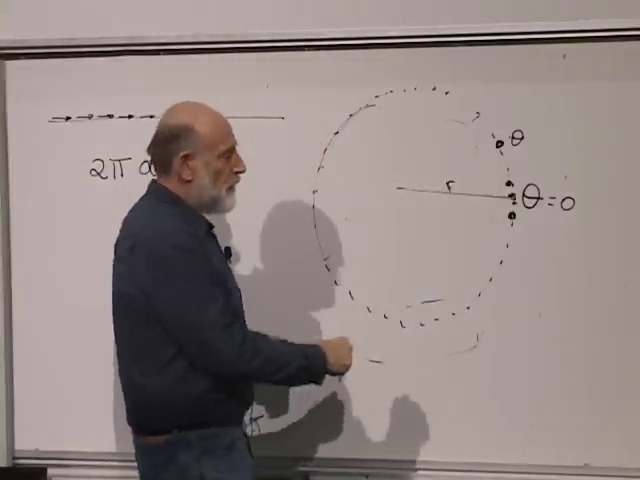
\includegraphics[width=0.82\textwidth]{lecture_01_figure_03.png}
\caption{Угловое описание замкнутой одномерной вселенной с полной длиной окружности \(2\pi a\).}
\end{figure}

Удобно принять следующее обозначение\footnote{Около 01:26:40--01:29:20 обозначения ненадолго переходят от того, чтобы принимать саму полную длину окружности за масштабный фактор, к записи её как \(2\pi a\). Здесь используется второй вариант, потому что именно он входит в формулу длины дуги.}:
\begin{equation}
L=2\pi a,
\end{equation}
где \(L\) — полная длина окружности.

Для малого углового расстояния \(\Delta\theta\) физическое расстояние равно
\begin{equation}
d=a\,\Delta\theta.
\end{equation}
Переходя к бесконечно малым, получаем
\begin{equation}
ds=a\,d\theta,
\end{equation}
и, следовательно,
\begin{equation}
ds^2=a^2\,d\theta^2.
\end{equation}
Это локальная метрика на окружности.

Если \(a\) зависит от времени, замкнутая одномерная вселенная расширяется или сжимается. Для фиксированной пары галактик,
\begin{equation}
d(t)=a(t)\,\Delta\theta,
\end{equation}
следовательно,
\begin{equation}
\dot d=\dot a\,\Delta\theta
      =\frac{\dot a}{a}\,d.
\end{equation}
Закон Хаббла сохраняется и здесь, по крайней мере для пар, которые не настолько далеко разнесены, чтобы путь вокруг окружности в другую сторону стал неоднозначным.

Метрика пространства-времени принимает вид
\begin{equation}
d\tau^2=dt^2-a^2(t)\,d\theta^2.
\end{equation}
Если величина \(a\) постоянна, пространственно-временная картина представляет собой цилиндр. Если \(a\propto t\), получается конус. Если \(a(t)\) меняется более нерегулярно, рисунок становится похожим на вазу.

Если прокрутить картину назад, галактики будут оказываться всё ближе и ближе друг к другу. Если бы по окружности было \(360\) галактик, в поздние времена они были бы хорошо разнесены, раньше — очень близко друг к другу, а ещё раньше — ещё ближе. В конце концов это были бы уже не отдельные галактики, а ещё раньше — даже не отдельные атомы. Но в пространстве по-прежнему нет никакой особой точки.

Это самый ясный ответ на вопрос о том, где в этой модели произошёл Большой взрыв. Когда \(a(t)\to 0\), каждое расстояние \(a(t)\,\Delta\theta\) стремится к нулю. Вся Вселенная сжимается повсюду одновременно. Галактики не разлетаются из одного привилегированного места во внешнем пространстве. Меняется масштаб самой геометрии. В этом смысле ответ таков: везде.

\begin{classroomqa}
\audiencequestion{Вы сказали, что пространство-время искривлено. А если это цилиндр, оно искривлено?}\lecturetimestamp{01:38:04}
\lecturerresponse{Нет. Если бы это был цилиндр, оно не было бы искривлено. Это тот случай, когда величина \(a\) постоянна во времени. Оно выглядит искривлённым только потому, что нарисовано в пространстве большей размерности. Если его разрезать, его можно развернуть на плоскость без растяжения.}
\end{classroomqa}

После этого обсуждение переходит к конусу. Если \(a\propto t\), пространственно-временная картина — конус. Вне его вершины конус тоже плоский в том же внутреннем смысле: его можно развернуть в плоскость. Вершина отличается. Это коническая сингулярность.

Следующий шаг — геометрия сферической вселенной, а затем динамика, определяющая, как \(a(t)\) растёт или уменьшается.

\chapter{Ньютоновская космология и уравнение Фридмана}

В прошлый раз мы говорили о метрике пространства. Следующий вопрос — динамика: как масштабный фактор меняется со временем? Сначала немного геометрии, а затем ньютоновская космология. Уравнение Фридмана мы пока не будем выводить из общей теории относительности. Мы выведем его из уравнений Ньютона.

\section{Однородность, изотропия и зависящая от времени метрика}

Однородность и изотропия — основные предположения. Если Вселенная однородна и изотропна и при этом меняется со временем, то закон Хаббла верен всегда. В любой фиксированный момент времени скорость удаления пропорциональна расстоянию,
\begin{equation}
v = H(t)\,d.
\end{equation}
Эта пропорциональность линейна. Постоянство относится не ко времени, а к пространству: в любой данный момент один и тот же коэффициент пропорциональности действует всюду.

\begin{classroomqa}
\audiencequestion{Это означает линейную пропорциональность?}\lecturetimestamp{00:02:06}
\lecturerresponse{Да. При фиксированном времени скорость удаления линейно пропорциональна расстоянию. Коэффициент пропорциональности — это постоянная Хаббла. Вообще говоря, она зависит от времени, но не меняется от точки к точке в пространстве.}
\end{classroomqa}

Именно поэтому выражение ``постоянная Хаббла'' опасно. Она постоянна по отношению к положению в пространстве. По отношению ко времени она не постоянна.

Далее возникает естественный вопрос. Если пространство расширяется, почему тогда не расширяются и метровые стержни? Ответ состоит в том, что метровые стержни удерживаются силами, несравнимо более сильными, чем что-либо, связанное с космологическим расширением на атомных масштабах. Связанные объекты остаются связанными. Расширяется расстояние между достаточно несвязанными объектами, например между галактиками, достаточно далекими друг от друга, чтобы они не связывали друг друга достаточно сильно.

\begin{classroomqa}
\audiencequestion{Нет ли тут проблемы из-за того, что измерительные стержни тоже расширяются?}\lecturetimestamp{00:04:00}
\lecturerresponse{Нет. Измерительные стержни не расширяются. Расширяются координаты. Силы, которые удерживают метровые стержни вместе, гораздо сильнее эффектов, обусловленных расширением, поэтому обычные связанные объекты не расширяются вместе с фоном. Галактики, находящиеся достаточно далеко друг от друга, расходятся, а метровые стержни — нет.}
\end{classroomqa}

Можно даже вообразить крошечный дополнительный отталкивающий эффект между атомами. Но и это не разорвало бы стержень. Это лишь немного сдвинуло бы равновесное расстояние — так же, как небольшое дополнительное натяжение меняет положение равновесия жесткой пружины.

\begin{classroomqa}
\audiencequestion{Но ведь нельзя моделировать это как силу между точками, верно? Потому что иначе это было бы ускорение.}\lecturetimestamp{00:05:29}
\lecturerresponse{Можно вообразить небольшую дополнительную силу между атомами, но если она мала по сравнению с силами связи, то она лишь слегка смещает положение равновесия. Само по себе расширение не порождает обычного закона силы. Некоторые виды расширения можно моделировать через силу, а именно ускоренное расширение, но это мы обсудим позже.}
\end{classroomqa}

Поэтому полезно пользоваться координатами, встроенными в расширяющееся распределение вещества. Галактики, не имеющие дополнительного пекулярного движения, сохраняют одни и те же координатные значения. Со временем меняется соотношение между координатным расстоянием и физическим расстоянием, измеряемым в метрах. Это соотношение задается масштабным фактором \(a(t)\).

Для плоского пространства пространственная метрика может быть записана в виде
\begin{equation}
ds^2 = a(t)^2\left(dx^2+dy^2+dz^2\right).
\end{equation}
Здесь \(a\) — это фактическое расстояние, измеряемое в метрах, между соседними точками, координатное расстояние между которыми равно единице. Если Вселенная расширяется, \(a\) становится зависящим от времени.

Чтобы перейти к пространству-времени, начнем со специальнорелятивистской формы
\begin{equation}
d\tau^2 = dt^2 - ds^2,
\end{equation}
и подставим пространственную метрику. Получаем
\begin{equation}
d\tau^2 = dt^2 - a(t)^2\left(dx^2+dy^2+dz^2\right).
\end{equation}
Коэффициенты не зависят от положения в пространстве. Они зависят только от времени. В языке метрики это и есть утверждение однородности. Диагональная метрика имеет вид
\begin{equation}
g_{\mu\nu}=\mathrm{diag}\!\left(1,-a(t)^2,-a(t)^2,-a(t)^2\right).
\end{equation}
\editorialnote{Полная диагональная матрица, записанная здесь, соответствует устному описанию метрического тензора около 00:14:33. На кадре с доской элемент линии виден ясно, но полностью разборчивая матрица не читается.}

Внедиагональных членов нет. Нет ни \(dx\,dy\), ни \(dx\,dt\), ни других смешанных членов. Метрика почти так же проста, как метрика плоского пространства-времени. Особенность состоит в том, что сама связь между пространственными расстояниями и временем зависит от времени.

\begin{figure}
\centering
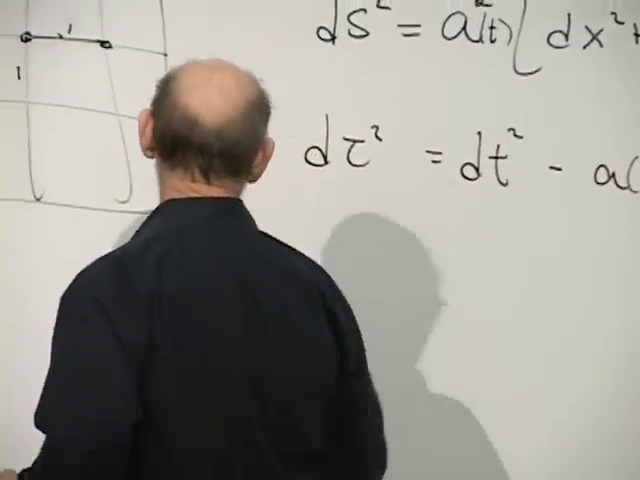
\includegraphics[width=0.62\textwidth]{lecture_02_figure_02.png}
\caption{Эскиз сопутствующей координатной сетки и пространственно-временной интервал с зависящим от времени масштабным фактором.}
\end{figure}

Рисунок передает суть. Алиса и Боб остаются на расстоянии одной единицы друг от друга в сопутствующих координатах, но эта одна координатная единица по мере течения времени соответствует все большему числу метров. Если бы \(a(t)\) в какой-то момент в прошлом был равен нулю, то всякое физическое расстояние было бы равно нулю. Все было бы сплющено одно на другое. Вот почему \(a\to 0\) соответствует бесконечной плотности. Если \(a\) растет, Вселенная становится все более разреженной.

Эта форма метрики справедлива не в любой системе отсчета. Это форма в системе отсчета, движущейся вместе с галактиками.

\begin{classroomqa}
\audiencequestion{В том уравнении маленькое \(t\) в \(a(t)\) — чье это \(t\)?}\lecturetimestamp{00:19:19}
\lecturerresponse{Это время, измеряемое часами, движущимися вместе с галактиками. Представьте себе одинаковые часы, изготовленные на одной и той же космической часовой фабрике и несомые галактиками. В этой системе отсчета временная переменная — в точности то, что измеряют эти часы. Вдоль мировой линии галактики собственное время совпадает с этим координатным временем.}
\end{classroomqa}

Действительно, вдоль мировой линии сопутствующей галактики,
\begin{equation}
dx=dy=dz=0,
\end{equation}
так что
\begin{equation}
d\tau^2 = dt^2,
\end{equation}
и, следовательно,
\begin{equation}
dt=d\tau.
\end{equation}

\begin{classroomqa}
\audiencequestion{Существуют ли преобразования, оставляющие эту форму метрики инвариантной?}\lecturetimestamp{00:23:08}
\lecturerresponse{Повороты — да, потому что \(dx^2+dy^2+dz^2\) инвариантно относительно поворотов. Но бусты Лоренца эту форму не сохраняют. Само вещество выделяет систему отсчета, движущуюся вместе с галактиками, и в какой-нибудь другой системе мир не выглядел бы изотропным.}
\end{classroomqa}

\section{Тело, брошенное в гравитационном поле}

Прежде чем применять механику Ньютона ко всей Вселенной, полезно вернуться к более простой задаче: тяжелая масса \(M\), гораздо меньшая масса \(m\) и начальный толчок наружу. После этого толчка малая масса просто движется в гравитационном поле и ведет себя так, как велят уравнения Ньютона.

Для космологического обсуждения важно не полное решение задачи об орбите. Важно сохранение энергии. Кинетическая энергия равна
\begin{equation}
\frac{1}{2}mv^2.
\end{equation}

\begin{figure}
\centering
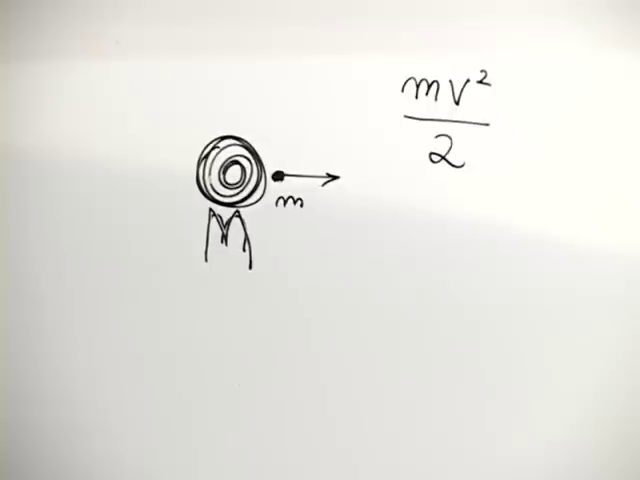
\includegraphics[width=0.42\textwidth]{lecture_02_figure_03.png}
\caption{Удаляющаяся пробная масса и член кинетической энергии \(\frac{1}{2}mv^2\).}
\end{figure}

Гравитационная потенциальная энергия содержит произведение масс, постоянную Ньютона и расстояние в первой степени в знаменателе. В записи на доске множители идут в порядке \(mMG/D\), поэтому лучше сохранить здесь этот порядок:
\begin{equation}
-\frac{mMG}{D}.
\end{equation}
Тогда полная энергия равна
\begin{equation}
\frac{1}{2}mv^2-\frac{mMG}{D}.
\end{equation}
Закон сохранения энергии утверждает лишь, что для рассматриваемой конкретной частицы эта величина не меняется со временем. У разных частиц энергии могут быть разными.

\begin{figure}
\centering
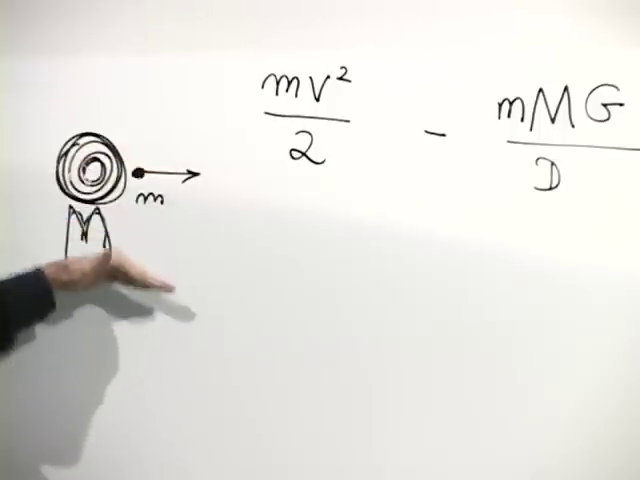
\includegraphics[width=0.62\textwidth]{lecture_02_figure_04.png}
\caption{Полная ньютоновская энергия для радиально движущейся пробной массы: кинетический член минус член гравитационной потенциальной энергии.}
\end{figure}

Отрицательный знак важен. Гравитационная потенциальная энергия отрицательна, потому что гравитация притягивает. Приближение частицы создает больше отрицательной потенциальной энергии. Перемещение ее дальше делает потенциальную энергию менее отрицательной.

\begin{classroomqa}
\audiencequestion{Потенциальная энергия растет с расстоянием, а не убывает?}\lecturetimestamp{00:34:13}
\lecturerresponse{Да. Отбросьте константы и посмотрите на графики \(1/D\) и \(-1/D\). Сила направлена в сторону убывания потенциальной энергии. Поэтому притягивающей силе соответствует перевернутая кривая, \(-1/D\), так что потенциальная энергия возрастает с расстоянием и становится более отрицательной, когда частица движется внутрь.}
\end{classroomqa}

\begin{figure}
\centering
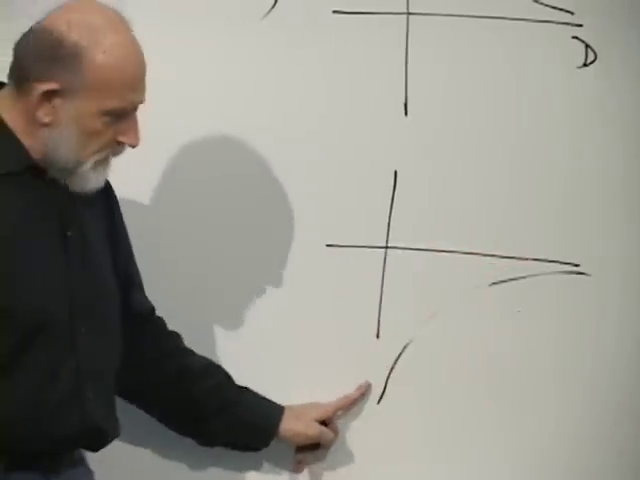
\includegraphics[width=0.46\textwidth]{lecture_02_figure_05.png}
\caption{Качественное сравнение \(1/D\) и \(-1/D\) для знака гравитационной потенциальной энергии.}
\end{figure}

\section{Скорость убегания}

Теперь классифицируем возможности. Энергия может быть положительной, отрицательной или нулевой. Это единственные три случая.

\begin{itemize}
\item Если энергия отрицательна, частица связана. Бросьте ее вверх со слишком малой скоростью, и она поднимется, замедлится, развернется и упадет обратно.
\item Если энергия положительна, частица убегает. Сначала гравитация замедляет ее, но недостаточно, чтобы остановить, и в конце концов она удаляется с ненулевой асимптотической скоростью наружу.
\item Если энергия в точности равна нулю, частица имеет скорость убегания. Это пограничный случай между тем, чтобы убежать, и тем, чтобы не убежать.
\end{itemize}

При достаточно малой начальной скорости с самого начала доминирует потенциальный член, и энергия отрицательна.

\begin{figure}
\centering
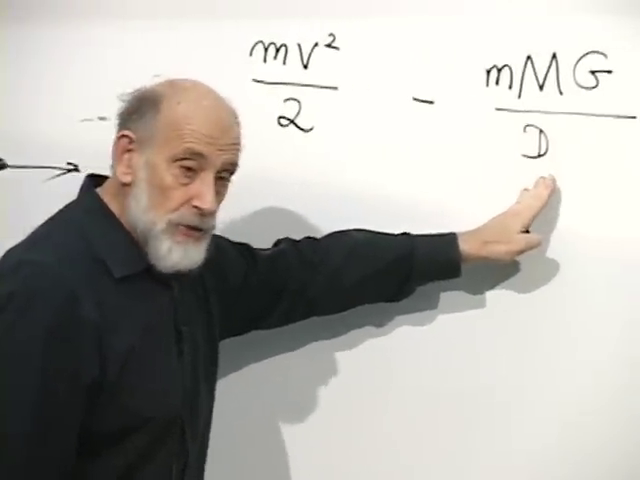
\includegraphics[width=0.62\textwidth]{lecture_02_figure_06.png}
\caption{При малой скорости наружу отрицательный потенциальный член доминирует в полной энергии.}
\end{figure}

В случае нулевой энергии расстояние продолжает увеличиваться, но скорость продолжает уменьшаться. Частица не может остановиться ни в какой конечный момент времени. Если бы это произошло, она упала бы обратно. Поэтому расстояние неограниченно, а скорость стремится к нулю.

Именно эта прямая аналогия важна для космологии. Вселенная может вести себя точно так же. Если начальный направленный наружу хаббловский поток достаточно велик, всё удаляется от всего остального. Если он слишком мал, побеждает гравитация и происходит гигантское сжатие. Есть и предельный случай, в точности аналогичный скорости убегания.

\section{Теорема Ньютона}

Космологическое сведение работает благодаря теореме Ньютона для закона обратных квадратов.

Если вещество распределено сферически симметрично относительно некоторого центра, то гравитационная сила, действующая на частицу вне этого распределения, в точности такая же, как если бы вся масса была сосредоточена в центре. Но теорема сильнее этого. Если частица находится внутри распределения, то вклад дает только масса на меньшем радиусе. Масса на большем радиусе не дает результирующей силы.

Самая ясная версия теоремы — тонкая оболочка. Идеальная сферическая оболочка не действует гравитационно на частицу нигде внутри нее, даже вдали от центра. На первый взгляд это удивительно, но для закона \(1/r^2\) это верно.

\begin{classroomqa}
\audiencequestion{В приведенном вами примере не должно ли нас немного удивлять то, что, когда частица пересекает границу, сила кажется разрывной?}\lecturetimestamp{00:48:19}
\lecturerresponse{Да. Для идеальной бесконечно тонкой оболочки это удивительно, и это свойственно именно закону силы \(1/r^2\). Реальная оболочка имеет толщину, поэтому изменение сглаживается, но резкое утверждение для идеальной оболочки и есть в точности замечательное свойство теоремы Ньютона.}
\end{classroomqa}

Тогда наглядный рисунок делает теорему правдоподобной. Замените точечную массу точечным источником воды. В трех измерениях поток наружу убывает как \(1/r^2\). Расположите такие источники непрерывно по всей сферической оболочке. Вне оболочки поток выглядит в точности так, как если бы всё было сосредоточено в центре. Внутри оболочки не может быть никакого результирующего потока, потому что в центре нет источника. Именно эта структура лежит и в основе гравитационной теоремы.

Смысл здесь не в том, чтобы заново выводить теорему. Смысл в том, чтобы ею пользоваться.

\section{Однородная Вселенная как задача об одном теле}

Теперь вернемся к космологии. Возьмите небольшой участок мира, заполненный однородным газом галактик. При желании можно считать себя находящимся в центре. Это лишь удобство. Любой может считать себя находящимся в центре, и должно получиться то же самое уравнение.

Выберите галактику на оси \(x\) с сопутствующей координатой \(x\). Поскольку Вселенная изотропна, выбор оси несуществен. Проведите сферу с центром в \(x=0\), проходящую через эту галактику. По теореме Ньютона сила, действующая на галактику, в точности такая же, как если бы вся масса внутри этой сферы была сосредоточена в центре, тогда как всё снаружи не давало никакого вклада.

Сфера расширяется вместе с галактиками. Она всегда содержит одни и те же галактики и, следовательно, ту же суммарную массу, хотя ее физический радиус меняется со временем.

Поэтому движение этой галактики подчиняется в точности такому же уравнению энергии, как и у снаряда:
\begin{equation}
\frac{1}{2}mv^2-\frac{mMG}{D}=\text{constant}.
\end{equation}
Здесь \(M\) теперь означает массу внутри расширяющейся сферы, а не центральную массу во вводном примере. Алгебра затем упрощается, если умножить на \(2\) и разделить на \(m\). Поскольку константа, деленная на \(m\), все равно остается просто константой, можно написать
\begin{equation}
v^2-\frac{2MG}{D}=\text{constant}.
\end{equation}
И снова ``константа'' означает константу по времени для данной конкретной галактики.

Теперь свяжем это с масштабным фактором. Физическое расстояние до галактики равно
\begin{equation}
D=ax,
\end{equation}
поскольку \(x\) — фиксированная сопутствующая координата. Скорость галактики равна
\begin{equation}
v=\dot D=\dot a\,x.
\end{equation}

Масса внутри сферы равна плотности, умноженной на объем. Если \(\rho\) — массовая плотность, то
\begin{equation}
M=\frac{4\pi}{3}\rho D^3=\frac{4\pi}{3}\rho a^3x^3.
\end{equation}
Подстановка в уравнение энергии дает
\begin{equation}
\dot a^2x^2-\frac{2G}{ax}\left(\frac{4\pi}{3}\rho a^3x^3\right)=\text{constant},
\end{equation}
или
\begin{equation}
\dot a^2x^2-\frac{8\pi G}{3}\rho a^2x^2=\text{constant}.
\end{equation}

Оба члена в левой части пропорциональны \(x^2\). Все остальное здесь одинаково повсюду. Следовательно, правая часть тоже должна быть пропорциональна \(x^2\). Это не противоречит тому, что ее называют константой. Это означает константу по времени для каждого фиксированного \(x\), но от одной галактики к другой она все же может масштабироваться как \(x^2\). В этом есть смысл. Более далекие галактики движутся быстрее.

Поэтому разделим на общий множитель \(x^2\). Оставшаяся константа теперь не зависит ни от времени, ни от пространства. Исторически стандартно обозначим ее как \(-k\):
\begin{equation}
\dot a^2-\frac{8\pi G}{3}\rho a^2=-k.
\end{equation}
После деления на \(a^2\)
\begin{equation}
\left(\frac{\dot a}{a}\right)^2=\frac{8\pi G}{3}\rho-\frac{k}{a^2}.
\end{equation}

Это знаменитое уравнение Фридмана—Робертсона—Уокера, хотя в лекции также замечается, что на самом деле это уравнение Фридмана. Соглашение о знаке историческое. То, что пишут \(-k\), не означает, что \(k\) должно быть положительным. \(k\) может быть положительным, отрицательным или нулем. В единицах, где скорость света положена равной \(1\), \(k\) безразмерно.

\section{Плотность и уравнение для случая доминирования вещества}

Следующий вопрос возникает сразу: что такое \(\rho\)? Это не константа. По мере расширения Вселенной плотность уменьшается.

Чтобы выразить эту зависимость, возьмите единичный куб в координатном пространстве: по одной единице по \(x\), \(y\) и \(z\). Внутри этого куба во все времена остаются одни и те же галактики, потому что куб расширяется вместе с координатной сеткой. Поэтому масса внутри этого координатного куба фиксирована.

\editorialnote{В лекции символ \(M\) используется повторно на нескольких этапах. Здесь \(M_{\Box}\) используется только для того, чтобы отличать массу в единичном координатном кубе от ранее встречавшихся центральной массы и массы, заключенной внутри сферы.}

Физическая длина ребра куба равна \(a\), так что его физический объем равен \(a^3\). Следовательно,
\begin{equation}
\rho=\frac{M_{\Box}}{a^3}.
\end{equation}
Это случай доминирования вещества: в правой части фигурирует только плотность обычного нерелятивистского вещества.

\begin{classroomqa}
\audiencequestion{Согласно этому уравнению, постоянная Хаббла является функцией \(\rho\). Следовательно, это не константа.}\lecturetimestamp{01:19:21}
\lecturerresponse{Именно. Постоянная Хаббла не является константой. Она зависит от плотности, а плотность меняется со временем. В лекции даже шутят, что итоговый экзамен мог бы состоять из одного вопроса: является ли постоянная Хаббла константой?}
\end{classroomqa}

Подстановка \(\rho=M_{\Box}/a^3\) в уравнение Фридмана дает
\begin{equation}
\left(\frac{\dot a}{a}\right)^2=\frac{8\pi G M_{\Box}}{3a^3}-\frac{k}{a^2}.
\end{equation}

На этом этапе уже ясно, какие величины выбираются произвольно. Нужно задать массу в единичном координатном кубе и значение \(k\). Трем возможным знакам \(k\) соответствуют три энергетических случая в задаче о снаряде.

\begin{itemize}
\item При \(-k>0\) энергия эффективно выше уровня, соответствующего скорости убегания, и Вселенная расширяется вечно.
\item При \(-k<0\) гравитация в конце концов побеждает, и Вселенная снова коллапсирует.
\item При \(k=0\) имеет место точный аналог скорости убегания.
\end{itemize}

\begin{classroomqa}
\audiencequestion{Если \(k=0\), то скорость между двумя галактиками стремится к нулю?}\lecturetimestamp{01:21:12}
\lecturerresponse{Да. В критическом случае скорость стремится к нулю, но расстояние все равно неограниченно. Галактики продолжают расходиться, только все медленнее и медленнее. Если бы они действительно остановились в какой-либо конечный момент времени, они упали бы обратно.}
\end{classroomqa}

\section{Критический случай \(k=0\)}

Теперь выберем простейший случай, \(k=0\). Это в точности случай скорости убегания, и он проще лишь потому, что проще математика. Уравнение принимает вид
\begin{equation}
\left(\frac{\dot a}{a}\right)^2=\frac{8\pi G M_{\Box}}{3a^3}.
\end{equation}

Правая часть всегда положительна и никогда не обращается в нуль. Следовательно, \(\dot a/a\) не может пройти через нуль. В этом случае Вселенная не может развернуться. Она либо всегда расширяется, либо всегда сжимается. Возьмем расширяющуюся ветвь.

Теперь предположим степенной закон,
\begin{equation}
a(t)=ct^p.
\end{equation}
Тогда
\begin{equation}
\dot a = cp\,t^{p-1},
\end{equation}
следовательно,
\begin{equation}
\frac{\dot a}{a}=\frac{p}{t}.
\end{equation}
Подстановка в дифференциальное уравнение дает
\begin{equation}
\frac{p^2}{t^2}=\frac{8\pi G M_{\Box}}{3c^3t^{3p}}.
\end{equation}
Чтобы степени \(t\) совпали, должно выполняться
\begin{equation}
3p=2.
\end{equation}
Значит,
\begin{equation}
p=\frac{2}{3}.
\end{equation}
Тогда для констант должно выполняться
\begin{equation}
\frac{4}{9}=\frac{8\pi G M_{\Box}}{3c^3},
\end{equation}
откуда
\begin{equation}
c^3=6\pi G M_{\Box}.
\end{equation}
Следовательно,
\begin{equation}
a(t)=\left(6\pi G M_{\Box}\right)^{1/3}t^{2/3}.
\end{equation}

При этом еще возможен аддитивный сдвиг времени. Он поглощается заменой \(t\) на \(t-t_0\). Как только выбирают начало отсчета времени так, что \(a=0\) при \(t=0\), эта оставшаяся константа исчезает.

Итак, Вселенная расширяется как время в степени две трети,
\begin{equation}
a(t)\propto t^{2/3}.
\end{equation}
Она не расширяется линейно со временем. Линейный рост был бы аналогом движения без ускорения. Здесь расширение замедляется.

Если продолжить формулу назад до \(t=0\), масштабный фактор стремится к нулю, а плотность неограниченно возрастает. Говорить \(a=0\) — это уже крайность. Мы не знаем, что происходит с веществом, когда оно становится слишком плотным. Реальный смысл в том, что на некоторой ранней стадии всё было настолько тесно упаковано, что атомы, ядра и кварки были тесно упакованы в чрезвычайно плотном состоянии.

\section{Постоянная Хаббла и возраст Вселенной}

В критической модели,
\begin{equation}
H(t)=\frac{\dot a}{a}=\frac{2}{3t}.
\end{equation}
Итак, постоянная Хаббла приблизительно равна величине, обратной возрасту Вселенной,
\begin{equation}
t=\frac{2}{3H}.
\end{equation}
Это один из главных результатов вычисления. Измерив сегодня постоянную Хаббла, мы получаем оценку возраста Вселенной, по крайней мере вплоть до того момента, когда ньютоновская модель перестает иметь смысл.

Указанный возраст составляет примерно от \(13\) до \(14\) миллиардов лет. В тексте также сказано, что \(k=0\) очень реалистично с точки зрения наблюдений: при указанной там точности никакого существенного отклонения от \(k=0\) не известно.

\begin{classroomqa}
\audiencequestion{Я просто немного запутался в том, что такое \(M\) и \(a\).}\lecturetimestamp{01:39:16}
\lecturerresponse{Обе величины содержат произвольность, связанную с выбором сетки. Если изменить условно выбранный ящик, изменится количество вещества в нем, и численное значение масштабного фактора тоже изменится. Физический смысл имеет плотность, \(M/a^3\), или, эквивалентно, комбинации вроде \(a/M^{1/3}\), которые не зависят от того, как выбрана сетка. В решении с \(k=0\) неизвестная постоянная, множащая \(t^{2/3}\), сокращается в \(\dot a/a\), так что соотношение для возраста \(t=2/3H\) не зависит от массы вещества в этом ящике.}
\end{classroomqa}

Это сокращение видно непосредственно из решения. Если
\begin{equation}
a(t)=Ct^{2/3},
\end{equation}
то
\begin{equation}
\dot a=\frac{2}{3}Ct^{-1/3},
\end{equation}
и, следовательно,
\begin{equation}
\frac{\dot a}{a}=\frac{2}{3t}.
\end{equation}
Постоянная \(C\) полностью сокращается.

\section{Почему ньютоновский вывод работает}

Ближе к концу возникает вопрос: почему ньютоновский вывод должен так хорошо согласовываться с релятивистским?

\begin{classroomqa}
\audiencequestion{Похоже, что все это зависит от предположения об открытой Вселенной.}\lecturetimestamp{01:45:44}
\lecturerresponse{На этом этапе вывод ньютоновский, а ньютоновская физика означает плоское пространство. Интерпретация \(k\) в терминах геометрии пространства отложена до следующей лекции. Там \(k=0\) будет соответствовать плоскому пространству, тогда как другие знаки будут связаны с искривленной пространственной геометрией.}
\end{classroomqa}

\begin{classroomqa}
\audiencequestion{Зависела ли когда-то очень давно длина метровых стержней от \(a\)?}\lecturetimestamp{01:47:53}
\lecturerresponse{Если уйти достаточно далеко в прошлое, вещество было бы настолько скучено, что отдельных метровых стержней на самом деле не существовало бы. А до того они были бы сжаты вместе. Лекция также напоминает, что теория относительности и так не допускает по-настоящему жестких тел: если бы тело было совершенно жестким, толчок с одной стороны мгновенно передавал бы сигнал на другую сторону, быстрее света.}
\end{classroomqa}

\begin{classroomqa}
\audiencequestion{Почему, как вы думаете, имеется такое совпадение между уравнениями — ньютоновским и релятивистским?}\lecturetimestamp{01:49:03}
\lecturerresponse{Потому что ньютоновское рассмотрение применяется лишь к достаточно малой области. Пока эта область мала по сравнению с радиусом кривизны всей Вселенной и пока локальные скорости Хаббла в ней значительно меньше скорости света, ньютоновская механика является хорошим приближением. В лекции это сравнивается с изучением роста травы на Земле: локальный процесс можно понять, не привлекая кривизну всей Земли.}
\end{classroomqa}

Это и есть логика локальной области. Ньютоновская механика предполагает, во-первых, что кривизна пространства не важна для рассматриваемого вопроса, и, во-вторых, что локально ничто не движется со скоростью, близкой к скорости света. В космологии это означает выбрать область, достаточно большую, чтобы быть однородной, но все же достаточно малую, чтобы эффектами кривизны можно было пренебречь и скорости Хаббла оставались нерелятивистскими.

Имея это в виду, ньютоновский расчет — не случайность. Это локальное приближение к уравнению, которое можно записать и в релятивистской форме. Если член кривизны перенести в левую часть, уравнение Фридмана принимает вид
\begin{equation}
\left(\frac{\dot a}{a}\right)^2+\frac{k}{a^2}=\frac{8\pi G}{3}\rho.
\end{equation}
Левая часть геометрична: в нее входят масштабный фактор и, как мы увидим в следующий раз, кривизна пространства. Правая часть — это плотность энергии. Именно такого рода уравнения и следует ожидать от общей теории относительности.

В следующий раз темой будут сама кривизна, уравнения Эйнштейна и связь между этим релятивистским выводом и ньютоновским.
\chapter{Фридмановское расширение, излучение и тёмная материя}

\section{Повторение основного космологического уравнения}

На масштабах, превышающих размеры скоплений галактик, Вселенную считают однородной. Выберем координаты так, чтобы мы находились в точке \(x=0\), и поместим типичную галактику, или просто воображаемую частицу, движущуюся вместе с потоком Хаббла, в точку \(x=1\). Тогда её физическое расстояние до нас по определению равно масштабному фактору \(a(t)\). Точка \(x=2\) находится на расстоянии \(2a(t)\), и так далее.

\begin{figure}[ht]
\centering
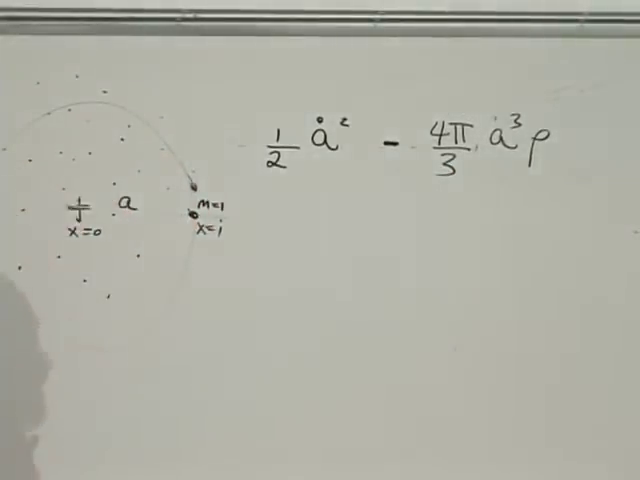
\includegraphics[width=0.78\textwidth]{lecture_03_figure_02.png}
\caption{Однородная сфера с центром в \(x=0\), сопутствующая галактика в \(x=1\) и ньютоновский баланс энергии для \(a(t)\).}
\end{figure}

Лишь вещество внутри сферы радиуса \(a(t)\) вносит вклад в гравитационное притяжение частицы в \(x=1\). Припишем этой частице единичную массу. Тогда её кинетическая энергия равна
\begin{equation}
\frac{1}{2}\dot a^2.
\end{equation}
Масса, заключённая внутри сферы, равна
\begin{equation}
M_{\mathrm{enc}}=\frac{4\pi}{3}a^3\rho,
\end{equation}
поэтому гравитационная потенциальная энергия равна
\begin{equation}
-\frac{G M_{\mathrm{enc}}}{a}
=
-\frac{4\pi G}{3}a^2\rho.
\end{equation}
\editorialnote{На отметке лекции 00:05:30 на доске отчётливо выписаны кинетический член и зависящий от плотности член потенциальной энергии. Полный коэффициент, записанный здесь, следует из устного вывода.}

Закон сохранения энергии даёт
\begin{equation}
\frac{1}{2}\dot a^2-\frac{4\pi G}{3}a^2\rho=\text{const}.
\end{equation}
Затем эту постоянную записывают как \(-k\), с обычным предупреждением, что стандартная нормировка на самом деле фиксирует это обозначение лишь после умножения уравнения на \(2\). В стандартной форме
\begin{equation}
\dot a^2=\frac{8\pi G}{3}a^2\rho-k,
\end{equation}
а деление на \(a^2\) даёт
\begin{equation}
\left(\frac{\dot a}{a}\right)^2=\frac{8\pi G}{3}\rho-\frac{k}{a^2}.
\end{equation}
Это уравнение Фридмана в форме, используемой на протяжении всего обсуждения.

\begin{figure}[ht]
\centering
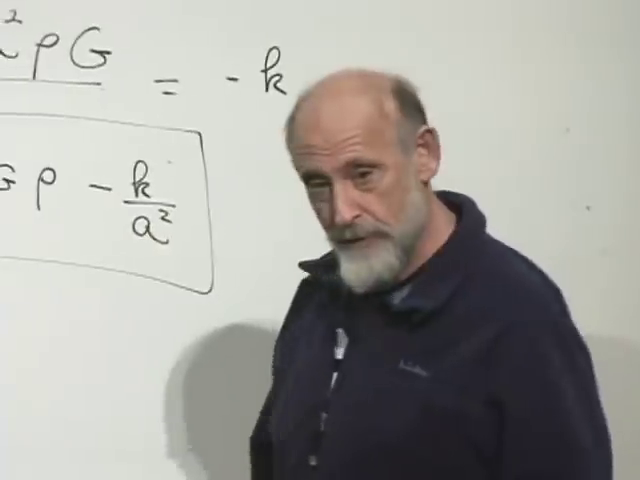
\includegraphics[width=0.56\textwidth]{lecture_03_figure_03.png}
\caption{Вклад кривизны \(-k/a^2\), выделенный в уравнении Фридмана.}
\end{figure}

Член кривизны по данным наблюдений очень близок к нулю, настолько близок, что на этом уровне его вполне можно просто пренебречь. Он действительно соответствует кривизне пространства, но наблюдательно здесь слишком мал, чтобы определить даже его знак.

Это же уравнение получается и из общей теории относительности. В схематическом виде уравнение Эйнштейна для компоненты время-время имеет вид
\begin{equation}
R_{00}-\frac{1}{2}g_{00}R \propto T_{00}.
\end{equation}
\editorialnote{Здесь в обсуждении приводится только тензорная структура, а не точный общий численный коэффициент.}
Для расширяющейся однородной метрики геометрическая часть даёт комбинацию \(\dot a/a\) и \(k/a^2\), тогда как материальная часть даёт плотность энергии. На этом этапе ньютоновский аргумент и уравнение Эйнштейна говорят одно и то же.

Это также меняет смысл \(\rho\). Начиная с этого места величину \(\rho\) лучше называть плотностью энергии. Для медленно движущегося вещества в сопутствующей системе отсчёта это просто плотность энергии покоя.

\section{Доминирование вещества}

Предположим теперь, что плотность энергии создаётся веществом, покоящимся в сопутствующей системе отсчёта. Рассмотрим куб со стороной в одну координатную единицу. Длины его рёбер равны \(a(t)\), так что его физический объём равен \(a^3(t)\). Если масса-энергия внутри этого сопутствующего куба равна \(M\) и вещество движется вместе с потоком, а не пересекает границу, то
\begin{equation}
\rho_m=\frac{M}{a^3}.
\end{equation}

Это случай доминирования вещества. В этой идеализации частицы покоятся в ящике, поэтому температуру принимают равной нулю и давление — нулевым. Давление потребовало бы, чтобы частицы пересекали границу ящика.

При \(k\approx 0\) уравнение принимает вид
\begin{equation}
\left(\frac{\dot a}{a}\right)^2=\frac{8\pi G}{3}\frac{M}{a^3}.
\end{equation}
Попробуем степенной закон,
\begin{equation}
a(t)=Ct^p.
\end{equation}
Тогда
\begin{equation}
\frac{\dot a}{a}=\frac{p}{t},
\end{equation}
поэтому левая часть масштабируется как \(t^{-2}\), а правая — как \(t^{-3p}\). Приравнивая показатели степеней, получаем
\begin{equation}
3p=2,
\qquad
p=\frac{2}{3}.
\end{equation}
Следовательно,
\begin{equation}
a(t)\propto t^{2/3}.
\end{equation}
Если сохранить коэффициент, то получаем
\begin{equation}
C^3=6\pi G M.
\end{equation}

Суть этого решения — степенной закон. Во Вселенной с доминированием вещества расширение идёт как время в степени две трети, а не линейно. Этот закон описывает длительную промежуточную эпоху — примерно от \(10^5\) лет после Большого взрыва до нескольких миллиардов лет спустя. Современная Вселенная не является в буквальном смысле веществодоминированной, поскольку теперь доминирует тёмная энергия, но обычное вещество и значительный промежуток космологической истории описываются именно так.

\section{Доминирование излучения}

Ещё раньше в плотности энергии доминировало излучение. Причина проста. Во Вселенной имеется огромное число фотонов, примерно \(10^9\) фотонов на каждый протон, и когда Вселенная сжимается, энергия этих фотонов возрастает.

У фотона нет массы покоя, но есть энергия. Его энергия равна
\begin{equation}
E_\gamma=h\nu=\frac{hc}{\lambda}.
\end{equation}
Ключевое предположение состоит в том, что при расширении Вселенной длины волн фотонов растягиваются вместе с ней:
\begin{equation}
\lambda\propto a.
\end{equation}
Верную картину даёт волна в ящике. Если ящик увеличивается, длина волны моды увеличивается вместе с ящиком. Та же идея используется здесь для расширяющейся Вселенной.

Поскольку \(\lambda\propto a\), энергия каждого фотона масштабируется как
\begin{equation}
E_\gamma\propto a^{-1}.
\end{equation}
Рассмотрим снова сопутствующий единичный ящик. Фотоны входят и выходят, но в среднем их число внутри остаётся постоянным. Тогда полная энергия фотонов в ящике тоже масштабируется как \(a^{-1}\). Разделив на физический объём \(a^3\), получаем, что плотность энергии излучения масштабируется как
\begin{equation}
\rho_r\propto a^{-4}.
\end{equation}

Вся разница сводится к этому дополнительному множителю \(a^{-1}\). Плотность вещества уменьшается, потому что Вселенная расширяется. Плотность излучения уменьшается по этой причине и ещё потому, что каждый фотон испытывает красное смещение.

Следовательно, уравнение Фридмана для Вселенной с доминированием излучения имеет вид
\begin{equation}
\left(\frac{\dot a}{a}\right)^2=\frac{8\pi G}{3}\frac{M_r}{a^4}.
\end{equation}
\editorialnote{В устном изложении символ \(M\) используется повторно для этой новой постоянной. Индекс \(r\) добавлен здесь только во избежание путаницы со случаем вещества.}

Воспользуемся той же пробной формой \(a(t)=Ct^p\). Левая часть снова масштабируется как \(t^{-2}\), а правая — как \(t^{-4p}\). Приравнивая показатели степеней, получаем
\begin{equation}
4p=2,
\qquad
p=\frac{1}{2}.
\end{equation}
Итак,
\begin{equation}
a(t)\propto t^{1/2}.
\end{equation}
Если сохранить коэффициент, то получаем
\begin{equation}
C^4=\frac{32\pi G}{3}M_r.
\end{equation}

\begin{classroomqa}
\lecturetimestamp{00:35:41}
\audiencequestion{Почему здесь появляется \(G\)?}
\lecturerresponse{Потому что гравитирует плотность энергии, а не одна лишь масса покоя. Для медленно движущегося вещества это различие легко упустить, но фотоны заставляют нас его учитывать: у них нет массы покоя, и всё же они гравитируют.}
\end{classroomqa}

Ящик, полный излучения, делает это наглядным. Толкните ящик, заполненный фотонами. Как только ящик начинает ускоряться, стенка, движущаяся навстречу фотонам, испытывает более сильные удары, чем стенка, удаляющаяся от них, так что приходится сильнее толкать, преодолевая давление излучения. Поэтому у ящика появляется дополнительная инерция, а по принципу эквивалентности эта дополнительная инерция означает и дополнительную гравитационную массу. Именно этот аргумент с ящиком фотонов здесь используется для утверждения, что энергия гравитирует.

\begin{classroomqa}
\lecturetimestamp{00:38:11}
\audiencequestion{Можно ли решить хотя бы одно из этих уравнений при \(a\), уменьшающемся со временем?}
\lecturerresponse{Да. Если восстановить член кривизны \(k/a^2\), существуют решения, которые расширяются, а затем сжимаются. По-видимому, наша Вселенная ведёт себя не так, но уравнение это допускает.}
\end{classroomqa}

\begin{classroomqa}
\lecturetimestamp{00:38:44}
\audiencequestion{Куда делось сохранение энергии?}
\lecturerresponse{Если восстановить член \(k\) и снова умножить уравнение на \(a^2\), космологическое уравнение в точности является законом сохранения. Вещество или излучение на одной стороне — лишь часть баланса. Расширение даёт кинетическую и гравитационную части, и полный баланс сохраняется.}
\end{classroomqa}

\section{Вещество и излучение вместе}

Реальная космология включает и вещество, и излучение. Их плотности масштабируются по-разному:
\begin{equation}
\rho_m\propto a^{-3},
\qquad
\rho_r\propto a^{-4}.
\end{equation}
Поэтому при малых \(a\) доминирует излучение. При больших \(a\) доминирует вещество. Следовательно, если идти назад по времени, ранняя Вселенная должна была быть с доминированием излучения.

\begin{figure}[ht]
\centering
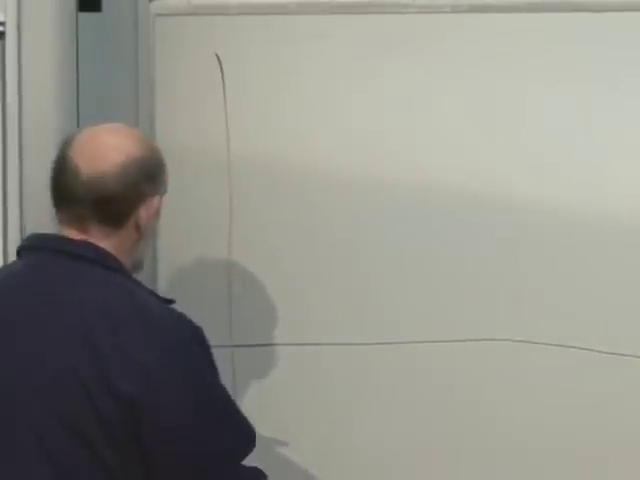
\includegraphics[width=0.68\textwidth]{lecture_03_figure_05.png}
\caption{Оси для сравнения плотностей энергии вещества и излучения как функций масштабного фактора.}
\end{figure}

\editorialnote{На отметке лекции 00:44:45 на доске в начале сравнительного графика показаны только оси. Кривые для вещества и излучения, обсуждаемые сразу после этого, описаны в тексте, а не перерисованы здесь.}

Кривая вещества убывает как \(a^{-3}\). Кривая излучения убывает как \(a^{-4}\). Обе расходятся при \(a\to 0\), но кривая излучения там растёт быстрее, поэтому две кривые пересекаются при масштабном факторе равенства. Грубая оценка помещает этот переход примерно через \(10^4\) лет, возможно, немного позже.

Ту же мысль можно выразить на графике \(a(t)\) в зависимости от \(t\). На ранней стадии расширение ведёт себя как \(t^{1/2}\). Позже — как \(t^{2/3}\). Изменение не является скачком; это непрерывный переход в сравнительно узком интервале времени.

\begin{classroomqa}
\lecturetimestamp{00:44:04}
\audiencequestion{По мере старения Вселенной непрерывно ли меняется показатель \(p\) от \(1/2\) к \(2/3\)?}
\lecturerresponse{Да. Он не изменяется скачком. Изменение непрерывно, хотя и происходит в довольно узком интервале времени.}
\end{classroomqa}

\section{Температура, рекомбинация и последнее рассеяние}

Следующая величина — температура. Если энергия типичного фотона масштабируется как \(a^{-1}\), то так же ведет себя и температура излучения:
\begin{equation}
T\propto a^{-1}.
\end{equation}
Если \(a\) удваивается, температура уменьшается вдвое.

Примем нынешнюю температуру фотонов равной примерно \(3\,\mathrm K\), а температуру ионизации — примерно \(3000\,\mathrm K\), то есть приблизительно температуре поверхности Солнца. Тогда
\begin{equation}
\frac{a_{\mathrm{today}}}{a_{\mathrm{ion}}}\sim 10^3.
\end{equation}
Используя закон позднего времени для эпохи доминирования материи \(a\propto t^{2/3}\),
\begin{equation}
\left(\frac{t_{\mathrm{today}}}{t_{\mathrm{ion}}}\right)^{2/3}\sim 10^3,
\end{equation}
получаем
\begin{equation}
\frac{t_{\mathrm{today}}}{t_{\mathrm{ion}}}\sim 1000^{3/2}\sim 3\times 10^4.
\end{equation}
Если принять возраст Вселенной на уровне этой оценки равным \(10^{10}\) лет, то получаем
\begin{equation}
t_{\mathrm{ion}}\sim 3\times 10^5\ \mathrm{years}.
\end{equation}

Это эпоха, когда водород и гелий перестают быть полностью ионизованными. До этого Вселенная представляет собой горячую плазму. Почему плазма непрозрачна? Потому что свободные заряды сильно откликаются на электромагнитные волны. Электрическое поле заставляет заряды колебаться туда-сюда, среда ведет себя как проводник, а проводники непрозрачны. Именно в этом состоит существенная аналогия с поверхностью Солнца.

Когда Вселенная остывает настолько, что электроны могут рекомбинировать с ядрами, образуются обычные нейтральные атомы, и она становится гораздо более прозрачной. Переход не является бесконечно резким. Это размытая область, или размытый интервал времени, но для космологии он достаточно резок, и потому его называют поверхностью последнего рассеяния.

Смотреть вдаль означает смотреть назад во времени. Близкие галактики показывают недавнее прошлое. Более далекие галактики показывают более ранние времена. На достаточно больших расстояниях любая линия зрения достигает эпохи, когда Вселенная была еще ионизованной и непрозрачной. Электромагнитное излучение не может показать ничего более раннего.

Другие носители информации в принципе могли бы зондировать более ранние времена. Нейтрино электрически нейтральны и отделились бы раньше. Гравитоны, если бы их когда-либо удалось наблюдать, приходили бы из еще более ранних эпох. Но та же слабость взаимодействия, которая позволила бы им проходить сквозь раннюю плазму, одновременно делает их чрезвычайно трудными для обнаружения.

Если когда-то во всех направлениях Вселенная была столь же горячей, как поверхность Солнца, почему же небо не ослепительно яркое? Потому что поверхность последнего рассеяния удаляется, и приходящие от нее фотоны испытали красное смещение примерно с тем же коэффициентом \(10^3\), который отделяет \(3000\,\mathrm K\) от \(3\,\mathrm K\). До нас доходит микроволновое излучение, а не видимый солнечный свет.

\begin{classroomqa}
\lecturetimestamp{01:03:51}
\audiencequestion{Значит, наши телескопы не могут заглянуть в эпоху раньше, чем примерно \(300{,}000\) лет?}
\lecturerresponse{Электромагнитные телескопы — не могут. До этого времени Вселенная была ионизованной и непрозрачной. Другие носители информации, по крайней мере в принципе, могли бы зондировать более ранние эпохи.}
\end{classroomqa}

\begin{classroomqa}
\lecturetimestamp{01:08:43}
\audiencequestion{Когда вы говорите о температуре фотона, вы имеете в виду температуру чёрного тела с таким максимумом излучения. Но это ведь не линейно по длине волны, верно?}
\lecturerresponse{Верно. Температура по существу задается энергией типичного фотона, так что для фотона она масштабируется обратно пропорционально длине волны. Закон \(T^4\) относится к плотности энергии, а не к энергии отдельного фотона. Он объединяет энергию на фотон с числом фотонов в единице объема, а численная плотность масштабируется как \(T^3\).}
\end{classroomqa}

Таким образом,
\begin{equation}
n_\gamma\propto T^3,
\qquad
\rho_\gamma\propto T^4.
\end{equation}

\section{Тёмная материя по кривым вращения}

Тёмная материя появляется здесь через галактические кривые вращения. О ее существовании заключили не из крупномасштабного уравнения Фридмана, а из астрономии на масштабах галактик.

Начнем с простейшей ньютоновской задачи: легкое тело массы \(m\) обращается вокруг центральной массы \(M\) по орбите радиуса \(r\). Сила тяготения равна
\begin{equation}
\frac{GMm}{r^2},
\end{equation}
а центростремительное ускорение равно \(v^2/r\). Закон Ньютона дает
\begin{equation}
m\frac{v^2}{r}=\frac{GMm}{r^2}.
\end{equation}
Сократив \(m\) и умножив на \(r\), получаем
\begin{equation}
v(r)=\sqrt{\frac{GM}{r}}.
\end{equation}
Итак, если гравитирующая масса сосредоточена вблизи центра, орбитальная скорость убывает как \(r^{-1/2}\).

Именно этого и следовало бы ожидать, если бы масса следовала за светом. Большая часть видимого вещества в галактике находится вблизи ядра, так что внешние звезды тогда вели бы себя примерно как планеты во внешней части Солнечной системы. Астрономы определяют орбитальные скорости, измеряя различия в доплеровском смещении по разные стороны близкой галактики: они сравнивают сторону, движущуюся к нам, с удаляющейся от нас, после вычитания общего рецессионного движения галактики как целого. Измеренные орбитальные скорости остаются примерно постоянными вплоть до больших радиусов.

Поэтому заменим центральную массу \(M\) массой, заключенной внутри радиуса, \(M(r)\):
\begin{equation}
\frac{v^2}{r}=\frac{G M(r)}{r^2}.
\end{equation}
Если \(v(r)\) приблизительно постоянна, то
\begin{equation}
M(r)\propto r.
\end{equation}
Иначе говоря, гравитирующая масса продолжает расти с радиусом даже там, где видимый свет уже не возрастает.

Теперь предположим, как и делается в обсуждении для простоты, что распределение массы приблизительно сферически симметрично. Тогда
\begin{equation}
M(R)=\int_0^R 4\pi r^2\rho(r)\,dr.
\end{equation}
Если \(M(R)\propto R\), то дифференцирование по \(R\) дает
\begin{equation}
4\pi R^2\rho(R)\propto 1,
\end{equation}
и, следовательно,
\begin{equation}
\rho(r)\propto \frac{1}{r^2}.
\end{equation}

\begin{classroomqa}
\lecturetimestamp{01:28:18}
\audiencequestion{Похоже, плотность должна вести себя как \(1/r^2\). Есть ли этому какая-то причина?}
\lecturerresponse{Из наблюдаемой плоской кривой вращения заключают, что \(M(R)\propto R\), а дифференцирование затем дает \(\rho(r)\propto 1/r^2\). Сверх этого здесь не утверждается никакого простого объяснения из первых принципов; большую часть работы выполняют детальные симуляции.}
\end{classroomqa}

Надежный вывод состоит в том, что галактика содержит гораздо больше гравитирующей массы, чем можно было бы заключить по одной лишь светящейся материи: по порядку величины — в несколько раз больше, а в используемой здесь оценке — примерно на порядок больше. Видимая галактика находится внутри намного большего тёмного гало.

Что мешает обычному газу оставаться в таком разреженном состоянии? Диссипация. Газовое облако сжимается, потому что столкновения, процессы, подобные трению, и излучение позволяют ему терять энергию. Тёмная материя, по-видимому, не излучает сколько-нибудь заметно и почти бесстолкновительна. Гравитация может стягивать ее внутрь и превращать потенциальную энергию в кинетическую, но без эффективной диссипации она не коллапсирует в компактные светящиеся структуры, которые образует обычная материя. То, что удерживает гало протяженным, — это кинетическая энергия.

Затем с осторожностью обсуждаются несколько альтернатив. Говорится, что нейтрино слишком быстры, чтобы вести себя так на галактических масштабах. Гало, состоящее из обычного водорода, сильно нарушило бы нуклеосинтез в ранней Вселенной. Черные дыры, образованные из обычной материи, тоже упоминаются как проблематичные, поскольку они означали бы слишком большое количество обычной материи в ранней Вселенной и породили бы проблемы с линзированием; большего здесь обсуждение и не утверждает.

Гало не описывается как тонкая оболочка или тор. Это приблизительно сферический, неоднородный шар, плотность которого выше к центру и постепенно падает наружу.

\begin{classroomqa}
\lecturetimestamp{01:53:12}
\audiencequestion{Вы говорите о Bullet Cluster?}
\lecturerresponse{Да. Газ, видимый в рентгеновских лучах, показывает обычную материю, тогда как линзирование показывает полную гравитирующую массу. При столкновении эти два распределения разделяются. Это сильное свидетельство в пользу реальной тёмной материи, а не просто модификации гравитации, привязанной только к видимой материи.}
\end{classroomqa}

Это последний наблюдательный аргумент. О том, что именно представляет собой тёмная материя, в деталях известно очень мало, но ничто здесь не требует радикально нового принципа. Консервативная возможность состоит просто в том, что в природе есть дополнительные слабо взаимодействующие частицы, которые пока еще не идентифицированы.
\chapter{Горизонты, уравнение состояния и энергия вакуума}

\section{Выделенная система отсчета, сверхсветовое удаление и горизонт}

Космический микроволновой фон действительно выделяет особую систему отсчета. В системе отсчета, в которой это излучение выглядит изотропным, окрестные галактики тоже в среднем покоятся. Если мы движемся сквозь фон, то фотоны в направлении вперед доплеровски смещаются к более высоким энергиям, а фотоны в обратном направлении — к более низким. Выделенная система отсчета — это та, в которой микроволновой фон выглядит изотропным; это также, в среднем, система отсчета, в которой покоятся окрестные галактики.

\begin{classroomqa}
\lecturetimestamp{00:00:25}
\audiencequestion{Зависит ли наблюдаемая длина волны космического излучения от движения наблюдателя и означает ли это существование выделенной системы отсчета?}
\lecturerresponse{Да. Движение сквозь микроволновой фон порождает доплеровскую анизотропию, так что существует выделенная космологическая система отсчета: та, в которой микроволновой фон выглядит изотропным. Это также, в среднем, система отсчета, в которой покоятся окрестные галактики.}
\end{classroomqa}

Второй вопрос касается скоростей удаления. Закон Хаббла утверждает, что достаточно далекие галактики удаляются согласно
\begin{equation}
v = H d .
\end{equation}
Для достаточно больших \(d\) эта скорость удаления превышает скорость света. Это не противоречит теории относительности, потому что запрет носит локальный характер: один объект не может пройти мимо другого прямо у нас перед глазами со скоростью, большей скорости света. Утверждение о далеких галактиках — это утверждение о геометрии между далеко разнесенными областями.

\begin{classroomqa}
\lecturetimestamp{00:04:48}
\audiencequestion{Могут ли две галактики иметь относительную скорость, большую \(c\)?}
\lecturerresponse{Да, если они достаточно далеко разнесены. Хаббловское удаление может превышать скорость света, не нарушая локальной теории относительности, а место, где скорость удаления достигает \(c\), — это горизонт.}
\end{classroomqa}

Когда скорость удаления достигает скорости света, сигналы, посланные к нам, в суммарном итоге больше не продвигаются к нам. Луч по-прежнему локально движется с предельной скоростью, но расстояние, которое ему нужно преодолеть, растет слишком быстро.

\begin{classroomqa}
\lecturetimestamp{00:07:03}
\audiencequestion{Разве световой луч, посланный в обратном направлении, все равно не будет идти к нам?}
\lecturerresponse{Локально будет, но пространство растет быстрее, чем луч способен это преодолеть. Луч движется с предельной скоростью относительно соседних точек, тогда как полное расстояние до нас продолжает увеличиваться.}
\end{classroomqa}

\section{Расширяющаяся метрика и аналогия с линией}

Полезная наглядная картина здесь одномерна. Представьте себе линию, состоящую из атомов. Если растягивать обычную материальную линию, она в конце концов порвется. Теперь изменим картину: всякий раз, когда соседние атомы слишком сильно раздвигаются, мы вставляем между ними еще один. Линия продолжает расти, но ее локальная структура не становится более разреженной.

\begin{figure}
\centering
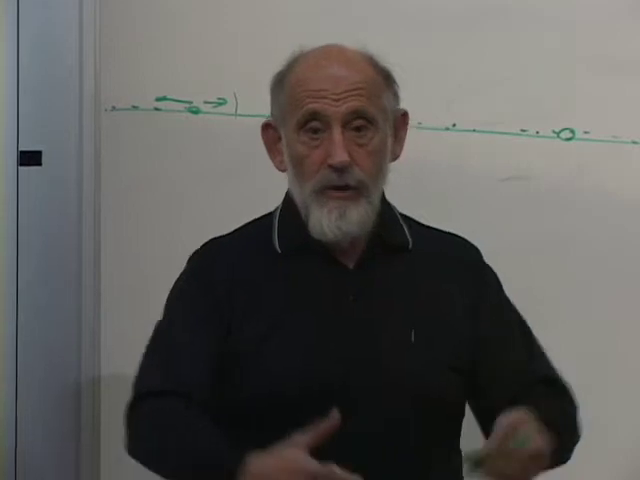
\includegraphics[width=0.60\textwidth]{lecture_04_figure_02.png}
\caption{Одномерная линия, используемая для наглядного изображения расширяющейся метрики.}
\end{figure}

В этой картине по-прежнему существует локальная предельная скорость сигнала, подобно тому как звук в обычной линии имеет предельную скорость. Правило локально: возмущение не может обогнать эту скорость относительно соседних точек. Тем не менее, если линия достаточно длинна и новые точки вставляются достаточно быстро, ее достаточно удаленные части удаляются так быстро, что сигнал никогда не сможет вернуться.

Поэтому специальнорелятивистский закон сложения скоростей — лишь часть картины. Он применим локально, когда наблюдатели проходят мимо друг друга в одной и той же точке. Для далеко разнесенных галактик в расширяющейся геометрии это не тот инструмент, который нужен.

\begin{classroomqa}
\lecturetimestamp{00:09:42}
\audiencequestion{Сохраняет ли в этой ситуации силу обычный релятивистский закон сложения скоростей?}
\lecturerresponse{Локально, в одной точке, да. Если наблюдатели последовательно проходят мимо друг друга, то действует обычное специальнорелятивистское правило. Но это не подходящий способ описывать удаление далеко разнесенных галактик со скоростью больше \(c\); здесь нужно вернуться к геометрии расширяющегося пространства.}
\end{classroomqa}

Та же картина дает простое объяснение красного смещения. Нарисуйте на линии волну. По мере расширения линии длина волны растет вместе с ней. В расширяющейся геометрии это не просто наглядный образ. Волновые уравнения в расширяющемся пространстве-времени действительно приводят к увеличению длины волны.

\begin{classroomqa}
\lecturetimestamp{00:14:42}
\audiencequestion{Является ли утверждение о том, что волна растягивается вместе со Вселенной, теоретическим, эмпирическим или и тем и другим?}
\lecturerresponse{Это теоретическое следствие распространения волн в расширяющемся пространстве-времени, и оно также подтверждается астрономическими наблюдениями.}
\end{classroomqa}

Эта картина — не резиновая лента. Резиновая лента при растяжении истончается, и тот, кто жил бы в такой среде, увидел бы изменение локальных свойств. Здесь же локальные свойства остаются теми же, тогда как глобальный масштаб расстояний растет.

\section{Последнее рассеяние и наблюдаемая Вселенная}

Горизонт — это место, где скорость удаления достигает скорости света. Поверхность последнего рассеяния лежит немного внутри него. Сигнал, испущенный с горизонта, растягивался бы неограниченно; излучение последнего рассеяния имеет огромное, но конечное красное смещение.

\begin{classroomqa}
\lecturetimestamp{00:17:53}
\audiencequestion{Какова связь между сверхсветовым удалением, поверхностью последнего рассеяния и наблюдаемой Вселенной?}
\lecturerresponse{Горизонт находится там, где скорость удаления достигает скорости света. Поверхность последнего рассеяния лежит немного внутри него, потому что ее красное смещение огромно, но конечно. Для практических целей она отмечает границу наблюдаемой Вселенной.}
\end{classroomqa}

Красное смещение излучения последнего рассеяния составляет приблизительно \(10^3\). Эта величина уже настолько велика, что поверхность последнего рассеяния для многих целей находится очень близко к горизонту. Наблюдаемая Вселенная — это та часть Вселенной, из которой свет может достичь нас.

На поздних стадиях расширение приближается к режиму, в котором доминирует энергия вакуума. Тогда величина Хаббла стремится к постоянной, горизонт стремится к фиксированному размеру, а и галактики, и микроволновое излучение постепенно исчезают из виду.

\begin{classroomqa}
\lecturetimestamp{00:22:43}
\audiencequestion{Поскольку \(H\) меняется со временем, меняется ли расстояние до горизонта и исчезнет ли в конце концов микроволновой фон?}
\lecturerresponse{На поздних стадиях \(H\) стремится к постоянной, так что горизонт стремится к фиксированному расстоянию. Микроволновой фон продолжает растягиваться, остывать и угасать. Далекие галактики тоже пересекают горизонт и исчезают из виду.}
\end{classroomqa}

Видимыми остаются только структуры, которые уже гравитационно связаны. Солнечная система не разлетается, и галактика не разлетается, но крупномасштабная Вселенная превращается в изолированный остров.

\section{Основное уравнение расширения и три компоненты}

Теперь основное уравнение расширения имеет вид
\begin{equation}
\left(\frac{\dot a}{a}\right)^2 = \frac{8\pi G}{3}\rho ,
\qquad c=1 .
\end{equation}
Здесь \(a(t)\) — масштабный фактор, а \(\rho\) — полная плотность энергии.

\begin{figure}
\centering
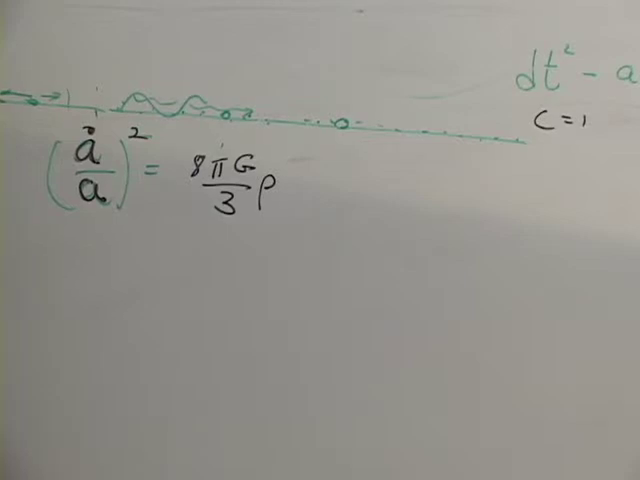
\includegraphics[width=0.74\textwidth]{lecture_04_figure_03.png}
\caption{Основное уравнение расширения и одномерная аналогия с линией.}
\end{figure}

Существуют три динамически важные компоненты.

Для материи,
\begin{equation}
\rho=\frac{\text{const.}}{a^3},
\qquad
a(t)\sim t^{2/3}.
\end{equation}
Это случай массивных объектов, участвующих в общем расширении и практически покоящихся в сопутствующей системе отсчета.

Для излучения,
\begin{equation}
\rho=\frac{\text{const.}}{a^4},
\qquad
a(t)\sim t^{1/2}.
\end{equation}
Дополнительная степень \(a\) обусловлена красным смещением каждого фотона по мере расширения Вселенной.

Есть также
\begin{equation}
\rho_0=\text{constant},
\end{equation}
энергия вакуума, также называемая темной энергией или, с точностью до общепринятых численных множителей, космологической постоянной. Эта компонента совсем не разрежается.

Следующий шаг — связать плотность энергии с давлением.

\section{Давление излучения и холодная материя}

Начнем с излучения. Рассмотрим одномерный ящик — просто отрезок длины \(L\), в котором фотоны движутся туда и обратно. В одном измерении сила и давление фактически совпадают.

Рассмотрим фотон с модулем импульса \(p\). При отражении от стенки его импульс изменяется на
\begin{equation}
\Delta p = 2p.
\end{equation}
Время между последовательными столкновениями с одной и той же стенкой равно
\begin{equation}
\Delta t = \frac{2L}{c}.
\end{equation}
Следовательно, средняя сила, действующая на стенку, равна
\begin{equation}
F=\frac{\Delta p}{\Delta t}=\frac{pc}{L}.
\end{equation}
Для фотона,
\begin{equation}
E=pc,
\end{equation}
так что
\begin{equation}
F=\frac{E}{L}.
\end{equation}
Энергия, деленная на длину, есть одномерная плотность энергии. В этом одномерном случае,
\begin{equation}
P=\rho .
\end{equation}

Для многих фотонов то же соотношение сохраняется и после усреднения. Полная сила — это просто полная энергия на единицу длины.

Теперь перейдём к трём измерениям. Если бы все фотоны двигались только вдоль одной оси, они оказывали бы давление на одну пару граней и не оказывали бы его на остальные. Это намеренно неверно, но сразу показывает, что нужно исправить. В изотропной ванне импульс распределён по всем направлениям. В среднем одна треть плотности энергии вносит вклад в каждую компоненту давления. Получаем
\begin{equation}
P=\frac{\rho}{3}.
\end{equation}

Для холодной материи ответ иной. Возьмём сопутствующий объём, небольшую область, движущуюся вместе с потоком Вселенной. Частицы внутри несут энергию, но если они покоятся относительно этого объёма, то не ударяются о его стенки. Поэтому давление равно
\begin{equation}
P=0.
\end{equation}

\begin{figure}
\centering
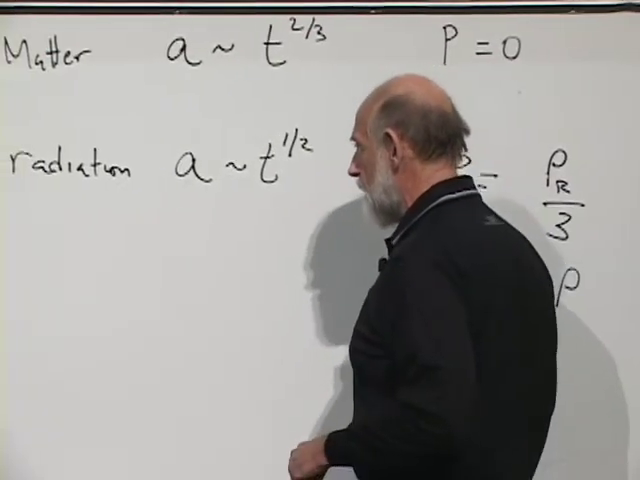
\includegraphics[width=0.74\textwidth]{lecture_04_figure_04.png}
\caption{Материя и излучение: \(a\sim t^{2/3}\), \(P=0\); \(a\sim t^{1/2}\), \(P=\rho/3\).}
\end{figure}

Итог на доске таков:
\begin{align}
\text{matter:}\qquad & a(t)\sim t^{2/3}, \qquad P=0,\\
\text{radiation:}\qquad & a(t)\sim t^{1/2}, \qquad P=\frac{\rho}{3}.
\end{align}

\begin{classroomqa}
\lecturetimestamp{00:54:27}
\audiencequestion{В расширяющейся Вселенной частицы ведь на самом деле разлетаются друг от друга?}
\lecturerresponse{Да, но рассуждение о давлении применяется к бесконечно малому сопутствующему объёму. На этом локальном масштабе термодинамическое рассуждение по-прежнему работает.}
\end{classroomqa}

\section{Уравнение состояния}

Предполагается, что давление пропорционально плотности энергии,
\begin{equation}
P=w\rho .
\end{equation}
На доске тот же параметр записан как \(\omega\). Для двух основных случаев
\begin{equation}
w=0 \quad \text{for cold matter},
\qquad
w=\frac{1}{3} \quad \text{for radiation}.
\end{equation}

Возможны и промежуточные случаи. Значения между \(0\) и \(1/3\) описывают вещество, которое не является ни полностью холодным, ни полностью релятивистским. Упомянутый здесь пример — тёплая тёмная материя.

\begin{figure}
\centering
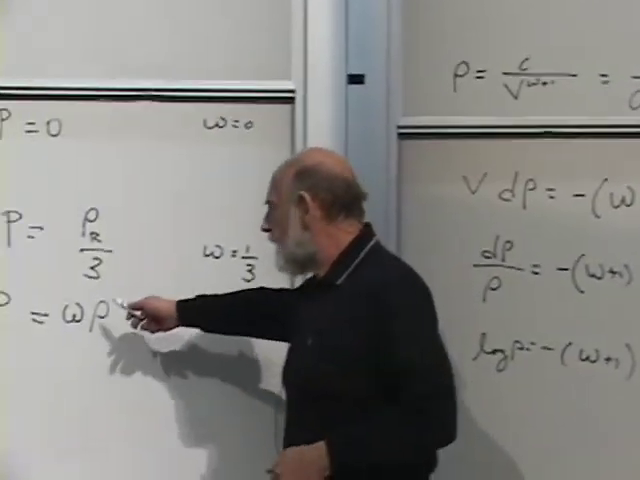
\includegraphics[width=0.74\textwidth]{lecture_04_figure_05.png}
\caption{Уравнение состояния \(P=\omega\rho\) и рассуждение о масштабировании плотности.}
\end{figure}

Следующий вопрос состоит в том, определяет ли \(w\) зависимость \(\rho\) от \(a\). Ответ следует из термодинамического тождества.

Возьмём ящик объёма \(V\). Если его содержимое оказывает давление \(P\), то при увеличении объёма ящика на \(dV\) работа, совершаемая над стенками, равна
\begin{equation}
dE=-P\,dV.
\end{equation}
Теперь запишем энергию в виде
\begin{equation}
E=\rho V.
\end{equation}
Её дифференциал равен
\begin{equation}
dE=\rho\,dV+V\,d\rho .
\end{equation}
Приравнивая эти два выражения, получаем
\begin{equation}
\rho\,dV+V\,d\rho=-P\,dV,
\end{equation}
или
\begin{equation}
V\,d\rho=-(\rho+P)\,dV.
\end{equation}
Используя \(P=w\rho\),
\begin{equation}
V\,d\rho=-(1+w)\rho\,dV.
\end{equation}
Разделим на \(\rho V\):
\begin{equation}
\frac{d\rho}{\rho}=-(1+w)\frac{dV}{V}.
\end{equation}
Интегрируя, получаем
\begin{equation}
\rho \propto V^{-(1+w)}.
\end{equation}
Для сопутствующего космологического объёма
\begin{equation}
V\propto a^3,
\end{equation}
и, следовательно,
\begin{equation}
\rho \propto a^{-3(1+w)}.
\end{equation}

Сразу получаются уже рассмотренные случаи:
\begin{align}
w=0 &\Longrightarrow \rho \propto a^{-3},\\
w=\frac{1}{3} &\Longrightarrow \rho \propto a^{-4}.
\end{align}

Вот почему важен \(w\). Как только известна \(\rho(a)\), её можно подставить обратно в уравнение Фридмана. Затем пробуют степенной закон \(a\sim t^\alpha\) и определяют, как расширяется Вселенная при таком уравнении состояния.

\section{Вакуумная энергия и отрицательное давление}

Один особый случай ведёт себя иначе:
\begin{equation}
w=-1.
\end{equation}
Тогда
\begin{equation}
1+w=0,
\end{equation}
так что показатель обращается в нуль и
\begin{equation}
\rho=\rho_0=\text{constant}.
\end{equation}
Соответствующее давление равно
\begin{equation}
P=-\rho .
\end{equation}

Отрицательное давление само по себе не является чем-то загадочным. Положительное давление толкает стенки ящика наружу. Отрицательное тянет их внутрь. Это натяжение. Обыденный пример — растянутая резинка: она запасает положительную энергию, но стягивает свои концы.

Подставим постоянную плотность \(\rho_0\) в уравнение Фридмана:
\begin{equation}
\left(\frac{\dot a}{a}\right)^2=\frac{8\pi G}{3}\rho_0.
\end{equation}
Правая часть — просто число, поэтому
\begin{equation}
\frac{\dot a}{a}=\sqrt{\frac{8\pi G}{3}\rho_0}.
\end{equation}
Это особый случай, в котором величина Хаббла действительно постоянна. Уравнение можно записать в виде
\begin{equation}
\dot a=\sqrt{\frac{8\pi G}{3}\rho_0}\,a,
\end{equation}
и его решение имеет вид
\begin{equation}
a(t)\propto \exp\!\left(\sqrt{\frac{8\pi G}{3}\rho_0}\,t\right).
\end{equation}

Это экспоненциальное расширение. Характерным масштабом времени здесь является время увеличения в \(e\) раз, а не время удвоения, и использованная здесь грубая оценка даёт величину порядка возраста Вселенной. Вакуумная энергия и космологическая постоянная — это одна и та же физическая составляющая, если не считать исторически сложившихся численных соглашений.

\begin{classroomqa}
\lecturetimestamp{01:27:16}
\audiencequestion{Если вакуумная энергия вызывает экспоненциальное расширение, разве в конце концов всё не будет разорвано?}
\lecturerresponse{Не обязательно. Связанные системы могут этому сопротивляться. Галактика, Солнечная система или атом не обязаны быть разорваны, тогда как достаточно большие и разрежённые структуры действительно участвуют в расширении и в конце концов расходятся.}
\end{classroomqa}

\begin{classroomqa}
\lecturetimestamp{01:31:43}
\audiencequestion{Есть ли что-нибудь интересное в отрицательном знаке, когда берут квадратный корень из уравнения Фридмана?}
\lecturerresponse{Да. Квадратный корень даёт две ветви. Одна — расширяющееся решение, а другая — обращённое по времени сжимающееся решение. Сами уравнения допускают обе.}
\end{classroomqa}

\section{Три эры и наблюдаемая история расширения}

Присутствуют все три компоненты, и масштабируются они по-разному:
\begin{equation}
\begin{aligned}
\rho_{\text{radiation}}&\propto a^{-4},\\
\rho_{\text{matter}}&\propto a^{-3},\\
\rho_0&=\text{constant}.
\end{aligned}
\end{equation}
Отсюда сразу следуют три эры.

При очень малых \(a\) доминирует излучение. Позже доминирует материя. При достаточно больших \(a\) доминирует вакуумная энергия. Соответствующие законы расширения имеют вид
\begin{equation}
a(t)\sim t^{1/2},
\qquad
a(t)\sim t^{2/3},
\qquad
a(t)\sim e^{Ht}.
\end{equation}

Приведённые здесь грубые времена таковы: примерно через \(10^4\) лет излучение уступает место материи. Позже, примерно через \(10^5\) лет, Вселенная становится прозрачной. Переход от доминирования материи к ускоренному расширению происходит намного позже, спустя несколько миллиардов лет, примерно на середине космической истории в используемой здесь оценке по порядку величины.

Как восстанавливают эту историю? Будущее мы видеть не можем, но прошлое можем. Смотреть на большие расстояния значит смотреть в более раннее время. Наблюдая далёкие галактики, измеряя, как их движение связано с расстоянием, и восстанавливая величину Хаббла как функцию времени запаздывания, восстанавливают временную зависимость масштабного фактора. Эра доминирования излучения слишком ранняя, чтобы её можно было непосредственно увидеть в обычной галактической астрономии, но эра доминирования материи и переход к доминированию вакуума видны на восстановленной кривой.

\section{Последнее рассеяние в далёком будущем}

Микроволновая картина неба в будущем — не то же самое, что исчезновение галактик за горизонтом. Излучение, которое мы видим в более поздние времена, приходит от более далёкого вещества, так что эффект состоит скорее в том, что мы заглядываем всё глубже и видим всё более холодное излучение, а не в том, что наблюдаем, как одни и те же атомы просто удаляются.

\begin{classroomqa}
\lecturetimestamp{01:48:07}
\audiencequestion{Если поверхность последнего рассеяния уходит в горизонт, то это то же самое, что галактики уходят за горизонт?}
\lecturerresponse{Нет. Более позднее излучение приходит не от тех же атомов, что излучение, которое мы видим сейчас. Оно приходит от атомов, которые находились дальше, так что это похоже на всё более глубокий взгляд во Вселенную, тогда как само излучение выглядит всё более холодным.}
\end{classroomqa}

\section{Кривизна, картина Большого схлопывания и горизонт на поздних временах}

До этого момента член с кривизной опускался. Если восстановить его, получаем
\begin{equation}
\left(\frac{\dot a}{a}\right)^2
=
\frac{8\pi G}{3}\rho
-
\frac{K}{a^2}.
\end{equation}
Численно этот член кажется малым, но концептуально он важен. На более старом ньютоновском языке он различает случаи положительной, нулевой и отрицательной полной энергии. На релятивистском языке он различает пространственные геометрии.

До того как к вакуумной энергии стали относиться всерьёз, часто представляли себе Вселенную, в которой доминирует материя и расширение в конце концов сменится сжатием. Отсюда возникала старая картина Большого схлопывания: расширение после Большого взрыва, а затем повторное сжатие. Математика по-прежнему верна, но больше не выглядит описанием нашей Вселенной.

\begin{classroomqa}
\lecturetimestamp{01:53:51}
\audiencequestion{Связана ли эта вакуумная энергия с квантовой энергией вакуума?}
\lecturerresponse{Да, или по крайней мере считается, что связана.}
\end{classroomqa}

Приблизительный сегодняшний состав таков:
\begin{equation}
\frac{\rho_0}{\rho_{\text{total}}}\sim 0.7,
\qquad
\frac{\rho_{\text{matter}}}{\rho_{\text{total}}}\sim 0.3.
\end{equation}
Внутри этой компоненты материи вклад светящейся материи составляет около \(0.05\), а тёмной материи — около \(0.25\) от общей плотности. Излучением сегодня можно пренебречь. Тёмная и светящаяся материя масштабируются одинаково, поэтому их отношение остаётся фиксированным, хотя относительная доля материи, излучения и вакуума меняется от эры к эре.

В пределе доминирования вакуума
\begin{equation}
H=\sqrt{\frac{8\pi G}{3}\rho_0}.
\end{equation}
Тогда закон Хаббла принимает вид
\begin{equation}
v=Hd.
\end{equation}
Горизонт определяется условием \(v=1\), поэтому его расстояние равно
\begin{equation}
d_H=\frac{1}{H}
=
\frac{1}{\sqrt{8\pi G\rho_0/3}}.
\end{equation}
Приведённая здесь грубая величина составляет примерно от \(10\) до \(12\) миллиардов световых лет.

Важно поведение на поздних временах. Как только расширение становится экспоненциальным, расстояние до горизонта фиксируется. Галактики продолжают пересекать его и исчезать по мере того, как их красный сдвиг всё растёт. Микроволновой фон тоже уходит в красный сдвиг. В очень далёком будущем видимыми останутся только близкие гравитационно связанные структуры, и Вселенная будет выглядеть как изолированный остров.

\section{Геометрия по поверхности последнего рассеяния}

Наконец, геометрию можно проверить по поверхности последнего рассеяния. Предположим, что расстояние до этой поверхности известно. Предположим также, что там можно выделить неоднородность, физический размер которой известен достаточно хорошо. Тогда можно сопоставить этот размер и это расстояние с наблюдаемым угловым размером.

В плоском пространстве угол совпадает с евклидовым. В пространстве положительной кривизны он казался бы больше; в пространстве отрицательной кривизны — меньше. Аналогия — с обычными геодезическими измерениями: взять объект известного размера на известном расстоянии и сравнить измеренный угол с предсказанием евклидовой геометрии.

\begin{classroomqa}
\lecturetimestamp{02:08:09}
\audiencequestion{Какой можно привести пример объекта там, размер которого нам известен?}
\lecturerresponse{Крупнейшие неоднородности микроволнового фона. Мы полагаем, что знаем их размер по тому, сколько времени заняла их эволюция, и по скорости звука.}
\end{classroomqa}

Здесь существенны крупнейшие неоднородности микроволнового фона. Их наблюдаемый угловой размер оказывается согласованным с евклидовой геометрией с точностью до нескольких процентов. На этом основании пространство представляется плоским.

\section{Измеренное значение \(w\) и заключительный вопрос}

Теперь ясна важность \(w\) для наблюдений. Если астрономы сообщают, что \(w\) очень близко к \(-1\), то они тем самым говорят, что компонента вакуумной энергии почти постоянна. Именно это здесь и утверждается.

Это не означает, что общая теория относительности вынуждает \(w\) быть в точности \(-1\). Суть здесь эмпирическая. В лекции кратко отмечается, что более радикальные возможности в принципе не исключены, но веские основания имеются именно в пользу случая почти постоянной вакуумной энергии.

\begin{classroomqa}
\lecturetimestamp{02:11:04}
\audiencequestion{При вычислении плотности для вещества и для излучения мы предполагали, что энергия постоянна, а затем подстраивали масштабный фактор, чтобы вывести формулу? И если это верно для первых двух случаев, то что происходит в случае вакуумной энергии, где плотность остается постоянной?}
\lecturerresponse{Нет. Я не предполагал, что она постоянна. Мы использовали то, что изменение энергии равно \(-P\,dV\). Для воображаемого сопутствующего ящика, движущегося вместе с расширением, на стенках совершается работа, и этим объясняется изменение энергии. Случай вакуумной энергии ставит вопрос по-иному, и заключительное замечание здесь состоит в том, что язык закона сохранения энергии в космологии мало что говорит, потому что полная энергия Вселенной равна нулю.}
\end{classroomqa}
\chapter{Сферы, гиперболическое пространство и смысл \(k\)}

Давайте немного займёмся математикой — простой математикой. Сферы в любом числе измерений — особые геометрии: они равномерны, и здесь равномерность означает постоянную кривизну. Сначала идёт положительная кривизна, затем равномерная отрицательная кривизна, а после этого — связь с уравнениями Эйнштейна.

Сферическая вселенная означает, что сферично \emph{пространство}, а не пространство-время. Есть и другая возможность — равномерная отрицательная кривизна. Именно сопоставление этих случаев делает ясной роль общей теории относительности.

\section{Сферы и равномерная геометрия}

1-сфера — это просто окружность. Проще всего описать её, вложив в двумерное вспомогательное пространство и записав
\begin{equation}
x^2+y^2=R^2.
\end{equation}
Единичная 1-сфера задаётся так:
\begin{equation}
x^2+y^2=1.
\end{equation}

2-сфера описывается точно так же, только теперь используются три вспомогательные координаты:
\begin{equation}
x^2+y^2+z^2=R^2,
\end{equation}
в единичном случае
\begin{equation}
x^2+y^2+z^2=1.
\end{equation}

Эти координаты — лишь вспомогательный приём. Интересующая нас геометрия — не окружающее пространство \(x,y,z\). Речь идёт о самой поверхности. Существо, живущее на 1-сфере, живёт на окружности; у него нет доступа ни к внутренней области, ни к внешней. Та же идея относится и к 2-сфере. Заполнение сферы и пространство вне неё принадлежат только вспомогательной картине.

Та же конструкция даёт 3-сферу. Вводят ещё одну координату, скажем \(w\), и пишут
\begin{equation}
x^2+y^2+z^2+w^2=R^2,
\end{equation}
а в единичном случае
\begin{equation}
x^2+y^2+z^2+w^2=1.
\end{equation}
3-сферу представить труднее, потому что теперь вспомогательное пространство было бы четырёхмерным, но сама математика не намного сложнее.

Стандартное обозначение — \(\Omega_n\) для \(n\)-сферы. Поэтому \(\Omega_1\) — это 1-сфера, \(\Omega_2\) — 2-сфера, а \(\Omega_3\) — 3-сфера.

\section{Метрики на сфере}

Более полезно внутреннее описание. Сферу описывают координатами, живущими на ней самой.

Для единичной 1-сферы достаточно одной координаты \(\phi\), причём \(0\leq \phi \leq 2\pi\). Её метрика имеет вид
\begin{equation}
ds^2=d\phi^2.
\end{equation}
Это также записывают как
\begin{equation}
d\Omega_1^2=d\phi^2.
\end{equation}

Единичную 2-сферу можно описать как семейство 1-сфер. Один угол \(\phi\) по-прежнему обходит каждую окружность, а второй угол \(\theta\) идёт от одного конца сферы до другого. Этот второй угол изменяется от \(0\) до \(\pi\). Движение в направлении \(\theta\) даёт вклад \(d\theta^2\). Движение в направлении \(\phi\) происходит по окружности радиуса \(\sin\theta\). Поэтому
\begin{equation}
d\Omega_2^2=d\theta^2+\sin^2\theta\,d\phi^2
\end{equation}
или
\begin{equation}
d\Omega_2^2=d\theta^2+\sin^2\theta\,d\Omega_1^2.
\end{equation}

3-сфера получается тем же способом, теперь как семейство 2-сфер. Введём ещё одну координату \(\alpha\). Тогда
\begin{equation}
d\Omega_3^2=d\alpha^2+\sin^2\alpha\,d\Omega_2^2.
\end{equation}
В развернутом виде это
\begin{equation}
d\Omega_3^2=d\alpha^2+\sin^2\alpha\left(d\theta^2+\sin^2\theta\,d\phi^2\right).
\end{equation}
Здесь \(\alpha\) пробегает от одного конца, где размер равен нулю, до другого, так что \(0\leq \alpha \leq \pi\).\editorialnote{В 00:17:24 в аудиозаписи на мгновение слышится ``от нуля до двух пи'', но окружающая конструкция и явный множитель \(\sin^2\alpha\) требуют, чтобы новая координата пробегала от одного конца семейства сфер меньшей размерности, где размер равен нулю, до другого.}

Общий рекурсивный вид таков:
\begin{equation}
d\Omega_n^2=d\alpha^2+\sin^2\alpha\,d\Omega_{n-1}^2.
\end{equation}

Как только принять эту точку зрения, о картине вложения можно забыть. 1-сфера описывается одной координатой, 2-сфера — двумя, 3-сфера — тремя и так далее. Геометрия существует сама по себе.

Эта геометрия особая, потому что она однородна. Можно было бы деформировать метрику, заменив \(\sin^2\theta\) какой-нибудь другой функцией, которая по-прежнему обращается в нуль на обоих концах. Тогда получилась бы некоторая деформированная замкнутая поверхность, например эллипсоид. Но она уже не была бы равномерной. Сфера однородна, потому что каждая точка на ней такая же, как любая другая.

Если нужна сфера радиуса \(A\), а не единичного радиуса, то единичную метрику умножают на \(A^2\):
\begin{equation}
ds^2=A^2\,d\Omega_3^2.
\end{equation}
Квадрат необходим, потому что метрика измеряет квадрат расстояния.

Короткое отступление касается 0-сферы. Экстраполируя на один шаг назад, получаем
\begin{equation}
x^2=1,
\end{equation}
у которого решениями являются две точки \(x=\pm 1\). Так что единичная 0-сфера — это просто две точки.

\section{Сферическая FRW-вселенная}

Теперь нас интересует не одно только пространство, а пространство-время. Соответствующая картина — это 3-сфера, радиус которой меняется со временем.

На всём протяжении важно одно предупреждение: время отлично от пространственных координат. Не следует представлять расширяющуюся Вселенную как сферу более высокой размерности, в которой время играет роль ещё одной координаты вложения.

Имея это в виду, интервал пространства-времени равен
\begin{equation}
d\tau^2=dt^2-a(t)^2\,d\Omega_3^2.
\end{equation}
Это метрика FRW для вселенной со сферической пространственной геометрией. Единственное новое обстоятельство по сравнению со статической сферой состоит в том, что радиус стал зависящей от времени функцией \(a(t)\).

Удобно выбрать координаты так, чтобы мы находились на одном из полюсов. В этой точке нет ничего особенного; это просто соглашение. Тогда \(\alpha\) можно рассматривать как радиальную координату, отсчитываемую от нас на единичной сфере. Это не радиальное расстояние в километрах. Это безразмерная угловая мера на единичной сфере, но в геометрии она играет роль радиального расстояния.

Если не считать локальных сгустков, таких как галактики и звёзды, то это и есть вся геометрия FRW-вселенной со сферической пространственной геометрией. Её пространственная кривизна положительна, и соответствующее соглашение о знаке записывается так:
\begin{equation}
k=+1.
\end{equation}
Само по себе здесь ничто не равно ``плюс одному''. Это просто означает положительную пространственную кривизну.

\section{Взгляд со сферы}

Как выглядит такая сфера, если смотреть с одной точки на ней? Здесь и появляется стереографическая проекция.

Возьмём 2-сферу, касающуюся бесконечной плоскости в южном полюсе. Выберем точку на сфере. Проведём прямую от северного полюса через эту точку и продолжим её, пока она не пересечёт плоскость. Так каждой точке на сфере ставится в соответствие точка на плоскости. Южный полюс переходит в начало координат на плоскости. Северный полюс — исключительная точка: при приближении к нему с разных направлений его образ уходит на бесконечность, причём по-разному в зависимости от направления. Поэтому его рассматривают как точку на бесконечности.

Если одинаковые ``континенты'' размещать в разных местах на сфере, то их изображения на плоскости становятся больше по мере приближения к северному полюсу. Поэтому наблюдатель, помещённый в южный полюс, видел бы дальние объекты под большими углами, чем в плоском пространстве. При положительной кривизне объект известного размера выглядит слишком большим по сравнению с евклидовой геометрией.

В этом и состоит основная наблюдательная идея. О кривизне судят по связи между расстоянием, размером и угловым размером. Сами галактики не очень хороши в качестве стандартных линеек на очень больших расстояниях, но логика именно такова.

\begin{classroomqa}
\lecturetimestamp{00:45:54}
\audiencequestion{Нужно ли также знать расстояние, а не только угловой размер?}
\lecturerresponse{Да. Одного угла недостаточно. Нужны и угол, и расстояние.}
\end{classroomqa}

\begin{classroomqa}
\lecturetimestamp{00:46:18}
\audiencequestion{Проецируются ли окружности на поверхности сферы в окружности?}
\lecturerresponse{Да. Окружности проецируются в окружности. Это одно из особых свойств стереографической проекции.}
\end{classroomqa}

\begin{classroomqa}
\lecturetimestamp{00:47:02}
\audiencequestion{Сохранил бы континент ту же форму при такой проекции?}
\lecturerresponse{Здесь есть два разных утверждения. Одно состоит в том, что окружности проецируются в окружности. Другое — более слабое — состоит в том, что достаточно малые фигуры сохраняют свою локальную форму, потому что углы сохраняются. Это отображение конформно: оно сохраняет углы, хотя и не относительные размеры.}
\end{classroomqa}

\section{Равномерная отрицательная кривизна}

Случай равномерной отрицательной кривизны вводится через его метрику.

Аналог сферы с отрицательной кривизной — гиперболическое пространство. В том же рекурсивном духе, что и раньше, его метрика получается заменой \(\sin\alpha\) на \(\sinh\alpha\):
\begin{equation}
d\mathcal H_n^2=d\alpha^2+\sinh^2\alpha\,d\Omega_{n-1}^2.
\end{equation}
Угловая часть меньшей размерности остаётся метрикой единичной сферы \(d\Omega_{n-1}^2\).

\begin{classroomqa}
\lecturetimestamp{00:55:51}
\audiencequestion{В метрике этот дифференциальный элемент меньшей размерности по-прежнему сферический?}
\lecturerresponse{Да. Этот фрагмент меньшей размерности — обычная метрика единичной сферы. Меняется множитель \(\sinh^2\alpha\) перед ним.}
\end{classroomqa}

Гиперболический синус равен
\begin{equation}
\sinh\alpha=\frac{e^\alpha-e^{-\alpha}}{2}.
\end{equation}
Знак минус важен; на лекции студент сразу же его исправляет.

Есть и еще одно важное различие в области значений координаты. Для сферы новая координата пробегает от одного конца до другого и останавливается на \(\pi\). Здесь
\begin{equation}
0\leq \alpha<\infty.
\end{equation}
Обычный синус возрастает, а затем вновь обращается в нуль. Гиперболический синус вблизи \(\alpha=0\) начинается так же, но затем растет экспоненциально.

Это означает, что окружающие нас сферы меньшей размерности становятся всё больше и больше по мере продвижения наружу. В этой геометрии небо на всё больших радиусах не сначала увеличивается, а потом уменьшается. Оно продолжает расти.

В трех пространственных измерениях соответствующая форма FRW имеет вид
\begin{equation}
d\tau^2=dt^2-a(t)^2\,d\mathcal H_3^2,
\end{equation}
а метка знака такова:
\begin{equation}
k=-1.
\end{equation}

\section{Дисковое представление и его смысл}

Отрицательная кривизна становится интуитивно понятной в дисковом представлении, прославленном Эшером, особенно \emph{Limit Circle Number Four}. Аналогия со стереографической проекцией полезна, но поведение здесь противоположное.

Для сферы проекция выглядит бесконечной, тогда как реальная геометрия конечна. В случае отрицательной кривизны дисковая картина выглядит конечной, тогда как реальная геометрия бесконечна. Равные ``континенты'' или ``галактики'' кажутся всё меньше и меньше по мере приближения к границе, но геометрически все они одного и того же размера. Если измерять расстояние, подсчитывая, сколько одинаковых частей пересекается, то граница находится бесконечно далеко.

Таким образом, в пространстве отрицательной кривизны знакомый объект выглядит слишком маленьким по сравнению с плоским пространством. Он виден под слишком малым углом.

Геометрия по-прежнему однородна. Хотя на этой картине внешние части кажутся крошечными, любой наблюдатель, оказавшийся в другом месте, увидел бы ту же самую внутреннюю геометрию.

\begin{classroomqa}
\lecturetimestamp{01:06:42}
\audiencequestion{Наблюдатель в любой из этих окружностей увидел бы похожую картину?}
\lecturerresponse{Да, в точности ту же самую. Пространство однородно.}
\end{classroomqa}

\begin{classroomqa}
\lecturetimestamp{01:07:03}
\audiencequestion{В сферическом случае далекие вещи кажутся слишком большими, а здесь — слишком маленькими?}
\lecturerresponse{Да. При положительной кривизне знакомый объект виден под слишком большим углом по сравнению с плоским пространством. При отрицательной кривизне он виден под слишком малым углом.}
\end{classroomqa}

\begin{classroomqa}
\lecturetimestamp{01:08:09}
\audiencequestion{Связано ли значение стереографоподобной проекции с тем, что астроном может восстановить ее по наблюдениям?}
\lecturerresponse{Да. Астроном, по существу, — геодезист, измеряющий треугольники на небе. Для данного геометрического вопроса зависимость от времени можно оставить в стороне и сосредоточиться на углах и расстояниях.}
\end{classroomqa}

Есть и полезная локальная картина. Небольшой участок отрицательной кривизны можно изобразить как седловую поверхность в обычном трехмерном пространстве. Но таким способом можно изобразить только малые участки; всю гиперболическую плоскость нельзя глобально вложить как обычную поверхность в трехмерное евклидово пространство.

\section{Плоский случай}

Между случаями положительной и отрицательной кривизны находится плоское пространство. О нем можно думать как о предельном случае, но достаточно просто иметь в виду обычное плоское евклидово пространство.

Его форма FRW имеет вид
\begin{equation}
d\tau^2=dt^2-a(t)^2\left(dx^2+dy^2+dz^2\right),
\end{equation}
при
\begin{equation}
k=0.
\end{equation}

Вот три однородные геометрии FRW:
\begin{align}
k=+1 &: \text{positive spatial curvature},\\
k=0 &: \text{flat space},\\
k=-1 &: \text{negative spatial curvature}.
\end{align}

\begin{classroomqa}
\lecturetimestamp{01:15:07}
\audiencequestion{Если спроецировать геометрию на плоскость и проследить сигнал, будет ли проецированная скорость света меняться от места к месту?}
\lecturerresponse{Да, на проекции она менялась бы. На сферической проекции казалось бы, что свет движется всё быстрее и быстрее по мере удаления; на диске отрицательной кривизны казалось бы, что у края он движется всё медленнее и медленнее. Это изменение относится к картинке, а не к лежащей в основе физике.}
\end{classroomqa}

\begin{classroomqa}
\lecturetimestamp{01:17:05}
\audiencequestion{Действительно ли такой способ рассмотрения далеких объектов использовался для определения плоскостности?}
\lecturerresponse{Да, но на деле используется именно угловая информация. Плоскостность не определяют, пытаясь измерить, с какой скоростью свет, как кажется, движется на проекции.}
\end{classroomqa}

\section{Возвращение к космологическим уравнениям}

После перерыва появляется связь между уже изученными космологическими уравнениями и уравнениями Эйнштейна. В этот момент на доске всё еще остается фрагмент плоской пространственной метрики.

\begin{figure}[htbp]
\centering
\includegraphics[width=0.72\textwidth]{lecture_05_figure_02.png}
\caption{Фрагмент плоской метрики FRW.}
\lectureframe{01:18:18}
\end{figure}

Сначала идет очень краткий ньютоновский обзор. Поместим себя в центр. Рассмотрим галактику, удаляющуюся согласно закону Хаббла. По теореме Ньютона для сферически симметричного распределения вклад в силу, действующую на нее, дает только масса внутри сферы, радиус которой равен расстоянию до галактики. Тогда есть три возможности: галактика движется со скоростью выше скорости убегания, ниже скорости убегания или точно со скоростью убегания.

Далее напоминается, что для обычного нерелятивистского вещества плотность ведет себя как масса, деленная на \(a^3\), для излучения — как \(1/a^4\), а для энергии вакуума она не меняется при изменении сферы.

В более раннем ньютоновском рассмотрении космологическое уравнение содержало член с плотностью и, если не находиться точно в случае скорости убегания, дополнительный постоянный член, пропорциональный \(1/a^2\). В предыдущем обсуждении этот член по большей части полагали равным нулю. Эмпирически он мал, но концептуально нет причин его опускать.

\section{Уравнения Эйнштейна и компонента \(00\)}

Следующий шаг — уравнения поля Эйнштейна. В левой части стоит геометрия, построенная из кривизны пространства-времени. В правой части стоит тензор энергии-импульса, источник гравитационного поля. В нормировке, используемой в лекции, пишут
\begin{equation}
R^{\mu\nu}-\frac{1}{2}g^{\mu\nu}R=4\pi G\,T^{\mu\nu}.
\end{equation}
\editorialnote{В видимой на доске строке коэффициент \(\tfrac12\) неразборчив, но около 01:33:36 устное исправление его восстанавливает. Здесь это уравнение сохраняет это исправление при сохранении лекционной нормировки \(4\pi G\).}

Здесь нужны не все десять независимых компонент. К этому моменту уже предположено так много --- однородность, форма FRW и единственный зависящий от времени масштабный фактор --- что остается только одна произвольная функция, а именно \(a(t)\). Естественно выбрать компоненту время-время, потому что \(T^{00}\) — это плотность энергии \(\rho\).

\begin{figure}[htbp]
\centering
\includegraphics[width=0.62\textwidth]{lecture_05_figure_05.png}
\caption{Уравнение поля Эйнштейна и его компонента \(00\).}
\lectureframe{01:30:54}
\end{figure}

Итак, в центре внимания стоит
\begin{equation}
R^{00}-\frac{1}{2}g^{00}R=4\pi G\,\rho.
\end{equation}

Правая часть — это плотность энергии. Левая часть — геометрия.

\begin{classroomqa}
\lecturetimestamp{01:39:09}
\audiencequestion{А как насчет других компонент тензора энергии-импульса?}
\lecturerresponse{Вообще говоря, они не обращаются в нуль. Пространственно-пространственные компоненты могут представлять давление. В случае доминирования вещества давление равно нулю, в случае доминирования излучения оно составляет одну треть плотности энергии, а для энергии вакуума пишут \(P=w\rho\) при \(w=-1\).}
\end{classroomqa}

\begin{classroomqa}
\lecturetimestamp{01:40:24}
\audiencequestion{Значит, если бы было только вещество, остальные компоненты \(T^{\mu\nu}\) обращались бы в нуль?}
\lecturerresponse{Для вещества без давления — да, компоненты давления обращаются в нуль.}
\end{classroomqa}

\section{Что дает вычисление по Эйнштейну}

Полный расчет кривизны на доске не проводится. Важно то, что получается, когда метрику FRW подставляют в тензор Эйнштейна.

Один тип члена возникает просто из того факта, что масштабный фактор зависит от времени. Даже если бы пространство было плоским, зависящий от времени масштабный фактор всё равно давал бы кривизну пространства-времени. Этот вклад пропорционален
\begin{equation}
\left(\frac{\dot a}{a}\right)^2.
\end{equation}

Второй тип члена возникает из самой пространственной кривизны. Даже если бы масштабный фактор не менялся со временем, искривлённое пространство всё равно вносило бы вклад в кривизну пространства-времени. Для простой геометрии постоянной кривизны кривизна ведёт себя как величина, обратная квадрату радиуса кривизны, так что она даёт член, пропорциональный
\begin{equation}
\frac{k}{a^2},
\end{equation}
со знаком плюс для сферы, со знаком минус для гиперболического случая и равный нулю для плоского пространства.

\begin{classroomqa}
\lecturetimestamp{01:36:53}
\audiencequestion{Не должен ли здесь также присутствовать такой множитель, как радиус кривизны?}
\lecturerresponse{Это уже и есть множитель \(1/a^2\). Для этих простых геометрий постоянной кривизны кривизна — это просто обратный квадрат радиуса кривизны.}
\end{classroomqa}

Учёт коэффициентов ведётся по ходу вывода и частично проверяется сравнением с полученным ранее ньютоновским ответом. В конечном итоге получаем\footnote{Эта выписанная форма уравнения Фридмана объединяет устное обсуждение коэффициентов с исправлениями по ходу изложения и сравнение с полученным ранее ньютоновским результатом на отрезке 01:32:35--01:36:53.}
\begin{equation}
\left(\frac{\dot a}{a}\right)^2+\frac{k}{a^2}=\frac{8\pi G}{3}\rho,
\end{equation}
или, эквивалентно,
\begin{equation}
\left(\frac{\dot a}{a}\right)^2=\frac{8\pi G}{3}\rho-\frac{k}{a^2}.
\end{equation}

Это именно та форма, которая связывает три геометрии FRW с рассмотренной ранее космологической динамикой.

\begin{classroomqa}
\lecturetimestamp{01:37:52}
\audiencequestion{Может ли \(k\) принимать любое значение, если переопределить \(a\)?}
\lecturerresponse{В плоском случае для \(a\) нет единственного естественного масштаба, так что его можно перемасштабировать, но \(k\) остаётся нулём. В сферическом случае и в случае отрицательной кривизны существует естественный масштаб кривизны. Если взять \(a(t)\) равным этому естественному радиусу кривизны, то \(k\) будет просто \(+1\) или \(-1\).}
\end{classroomqa}

\begin{classroomqa}
\lecturetimestamp{01:41:00}
\audiencequestion{Равно ли \(k\) в том последнем уравнении \(+1\), \(-1\) или \(0\)?}
\lecturerresponse{Да. Для сферы это \(+1\), для гиперболического случая \(-1\), а для плоского пространства \(0\).}
\end{classroomqa}

Ньютоновское рассмотрение не ввело нас в заблуждение; оно дало то же основное уравнение. То, что добавляет общая теория относительности, — это интерпретация. С ньютоновской точки зрения дополнительная константа различает случаи выше скорости убегания, ниже неё и пограничный случай. С точки зрения Эйнштейна тот же знак говорит нам о геометрии самого пространства.

\begin{classroomqa}
\lecturetimestamp{01:42:46}
\audiencequestion{Как это работало до включения космологической постоянной?}
\lecturerresponse{До введения космологической постоянной между режимом относительно скорости убегания и геометрией пространства существовала тесная связь. Если \(k=+1\), пространство имеет положительную кривизну, а движение соответствует случаю ниже скорости убегания, так что Вселенная может расширяться, а затем вновь сжиматься. Если \(k=-1\), пространство имеет отрицательную кривизну, а движение соответствует случаю выше скорости убегания, так что Вселенная продолжает расширяться. Если \(k=0\), имеет место предельный, пограничный случай.}
\end{classroomqa}

Следовательно, один и тот же знак \(k\) можно читать двумя способами: как динамическую классификацию движения и как знак кривизны пространства.

\chapter{Последнее рассеяние и бариогенез}

\section{Смотреть вдаль — значит смотреть в прошлое}

На разных расстояниях мы видим Вселенную в разные моменты времени. На малых расстояниях время, на которое мы заглядываем в прошлое, не очень существенно. Вселенная год назад или сто лет назад не слишком отличалась от Вселенной сейчас. Но на достаточно больших расстояниях мы видим Вселенную более молодой. Более молодая Вселенная плотнее, а более плотная — горячее.

На некотором достаточно большом расстоянии Вселенная была примерно такой же горячей, как поверхность Солнца. Нам она так не выглядит, потому что фотоны по пути к нам испытали красное смещение. Коэффициент красного смещения порядка тысячи означает наблюдаемую температуру, меньшую во столько же раз:
\[
T_{\mathrm{obs}} \sim \frac{T_{\mathrm{emit}}}{1+z},
\qquad
1+z \sim 10^3.
\]\footnote{Эта запись представляет собой сжатую редакторскую передачу словесного рассуждения о красном смещении из 00:02:20--00:02:39.}

Именно там Вселенная стала непрозрачной. Она состояла главным образом из водорода, с небольшой примесью гелия. При температуре выше нескольких тысяч градусов водород ионизован. Поэтому по ту сторону этой поверхности находятся не нейтральные атомы, а ионы: главным образом свободно движущиеся протоны и электроны. Фотоны там тоже более энергичны, по существу это рентгеновские фотоны. Если атом случайно образуется, столкновения или фотон быстро снова его ионизуют.

Ионизованный газ является электрическим проводником, а проводник не даёт излучению проходить беспрепятственно. Заряды реагируют на электрические поля, колеблются взад и вперёд и переизлучают его. Поэтому дальше этого расстояния Вселенная для нас непрозрачна. Поверхность последнего рассеяния подобна видимой поверхности Солнца: это не материальная стена, а место, где среда довольно резко переходит от непрозрачности к прозрачности.

Большинство частиц там — фотоны: их примерно в \(10^8\) раз больше. То же верно и сегодня, хотя сегодня энергия фотонов настолько мала, что они не составляют важной части современной плотности энергии. Когда температура падает ниже температуры ионизации водорода, Вселенная становится прозрачной, и мы можем видеть сквозь неё.

На этом прямое наблюдение заканчивается. Следующий вопрос состоит в том, насколько дальше в прошлое нас ещё позволяют продвинуться известные атомная, ядерная физика и физика элементарных частиц.

\section{Ещё дальше в прошлое}

Сразу по ту сторону поверхности последнего рассеяния, помимо фотонов, основными частицами являются протоны и электроны, а также некоторое количество ядер гелия и немного дейтронов. Антипротонов практически нет, и позитронов тоже практически нет. Но дальше в прошлое температура в конце концов становится достаточно высокой, чтобы два фотона могли столкнуться и породить электрон и позитрон:
\[
\gamma + \gamma \leftrightarrow e^- + e^+.
\]

Основной порог определяется тем, что фотоны должны по меньшей мере обеспечить энергию покоя пары:
\[
E \ge 2m_e c^2.
\]
Ниже этого порога обычного света недостаточно. Выше него могут рождаться электрон--позитронные пары, и обратная реакция тоже может происходить. В горячей порции вещества при такой температуре происходили бы реакции между частицами, играющие ту же роль, что химические реакции в обычном веществе.

Непосредственно выше порога фотонов всё ещё больше, чем электронов и позитронов. Масса покоя электрона энергетически дорога. Но когда температура становится намного выше порога, энергия покоя электрона оказывается менее важной, чем кинетическая энергия, и численные плотности становятся сравнимыми. Тогда электроны, позитроны и фотоны имеют примерно одинаковые численные плотности и сталкиваются с бешеной частотой.

\begin{figure}[ht]
\centering
\includegraphics[width=0.62\textwidth]{lecture_06_figure_02.png}
\caption{Схема порога рождения пар для сравнения масштабов масс электрона и протона.}
\lectureframe{00:18:47}
\end{figure}

Следующий вопрос — что происходит с протонами. Они уже присутствуют, и к этому времени их численная плотность очень велика, но тепловой энергии ещё недостаточно, чтобы в изобилии рождать протон--антипротонные пары. Причина проста:
\[
m_p \approx 2000\,m_e,
\qquad
E \ge 2m_p c^2
\]
— это гораздо более высокий порог.\editorialnote{На кадре нижняя подпись массы менее чёткая, чем верхняя \(2m_e c^2\), но в устном объяснении сравнение явно проводится между электронным и протонным порогами.}

Это уже намного горячее, чем внутри звезды, где античастицы не присутствуют в сколько-нибудь заметном количестве.

Но и это лишь предварительное описание. К тому времени, когда температура становится достаточно высокой, чтобы протоны и антипротоны свободно рождались, она уже достаточно высока и для того, чтобы разбивать протоны на кварки. Поэтому эту по-настоящему горячую среду лучше описывать как смесь электронов, позитронов, кварков, антикварков, фотонов, нейтрино, глюонов и других видов частиц. Простая схематическая реакция с доски такова:
\[
e^- + e^+ \to \gamma \to q + \bar q.
\]

\begin{classroomqa}
\lecturetimestamp{00:20:05}
\audiencequestion{Это мезоны или прекварки?}
\lecturerresponse{Мезоны состоят из кварков. Как только температура становится достаточно высокой, чтобы разрушить протон, она разрушает и мезоны.}
\end{classroomqa}

До сих пор рассуждение шло назад во времени. Теперь развернём его и спросим, что происходит, когда горячая симметричная смесь остывает.

\section{Электрическая нейтральность и горячая симметричная Вселенная}

При достаточно высокой температуре во Вселенной имеются колоссальные концентрации частиц и античастиц. Электроны и позитроны появляются парами, кварки и антикварки появляются парами, и естественно ожидать почти равных количеств каждой частицы и её античастицы.

Понятие электрической нейтральности требует некоторой осторожности. Сегодня Вселенная электрически нейтральна. Полезный мнемонический приём — представить не нашу реальную Вселенную, а замкнутую и ограниченную Вселенную, например трёхсферу. Сначала рассмотрим в качестве модели двумерную сферу. Силовые линии электрического поля не могут начинаться или заканчиваться нигде, кроме как на заряде. Положительный заряд испускает силовые линии; отрицательный их поглощает. На замкнутой сфере такие линии не могут просто уйти на бесконечность. Они снова сходятся на противоположной стороне. Поэтому в качестве мнемонического образа можно сказать, что замкнутая и ограниченная Вселенная не может иметь ненулевой суммарный заряд. Дело не в том, является ли наша реальная Вселенная в буквальном смысле замкнутой. Суть в том, что на больших масштабах положительные и отрицательные заряды, по-видимому, компенсируют друг друга чрезвычайно точно.

Электрическая нейтральность \emph{не} означает, что число протонов равно числу антипротонов. Она означает, что полный положительный заряд равен полному отрицательному заряду. Протоны, позитроны и все прочие положительно заряженные частицы вместе уравновешивают электроны и все прочие отрицательно заряженные частицы вместе.

Настолько далеко назад во времени, насколько можно доверять известной физике, и, возможно, немного дальше, Вселенная была достаточно горячей, чтобы в ней в изобилии существовали и частицы, и античастицы. Любому ускорительному эксперименту, какой только можно назвать, на каком-то этапе соответствовал аналог в ранней Вселенной. Почти симметричное начало — естественная гипотеза: равные числа электронов и позитронов, равные числа кварков и антикварков и, если протоны и антипротоны использовать в качестве представителей барионов и антибарионов,
\[
N_p = N_{\bar p}.
\]

Эта гипотеза привлекательна, потому что законы физики почти симметричны по отношению к частицам и античастицам. Позитрон ведёт себя почти так же, как электрон, не совсем, но очень близко. Именно эта почти симметрия и есть проблема.

\section{Прокручивая фильм вперёд}

Предположим, что Вселенная начинается в горячем состоянии с равными или почти равными количествами частиц и античастиц, а затем остывает.

Пока температура достаточно высока, протоны и антипротоны могут рождаться в энергичных столкновениях, и они могут аннигилировать обратно в фотоны. Но в конце концов температура опускается ниже протонного порога. Тогда протон--антипротонные пары ещё могут аннигилировать в фотоны, но после некоторого расширения эти фотоны теряют достаточно энергии и уже не могут снова превращаться в протон--антипротонные пары. Это улица с односторонним движением. То же самое позже происходит с электронами и позитронами, при температуре гораздо ниже протонного порога, но всё ещё намного выше звёздных температур.

Поскольку расширение происходит медленно по сравнению со скоростями микроскопических реакций, во время этого процесса Вселенная большую часть времени остаётся близкой к тепловому равновесию. Именно это здесь и имеется в виду под адиабатическим расширением. В этих условиях точнее говорить, что энтропия меняется очень мало. Для горячей смеси частиц энтропия по существу определяется числом частиц, с точностью до множителей порядка единицы. Так что протоны, антипротоны, электроны и позитроны, которые аннигилируют, приблизительно заменяются фотонами.

Если бы числа протонов и антипротонов были в точности равны, они просто полностью аннигилировали бы. То же самое произошло бы с электронами и позитронами. Остались бы фотоны. Но если бы существовал хотя бы крошечный избыток протонов над антипротонами, все образовавшиеся пары аннигилировали бы, а неспаренный избыток остался бы. Конкретный пример проясняет мысль: если бы было сто протонов и пятьдесят антипротонов, то эти пятьдесят антипротонов нашли бы пятьдесят протонов, аннигилировали бы с ними, и осталось бы пятьдесят протонов. Тогда нейтральность заряда требует такого же рода оставшегося избытка электронов над позитронами.

Это позволяет восстановить раннюю асимметрию по нынешнему числу фотонов. Сегодня число фотонов примерно от \(10^9\) до \(10^{10}\) раз больше числа протонов или электронов:
\[
\frac{N_\gamma}{N_p} \sim 10^9\text{--}10^{10}.
\]
Следовательно, в раннем горячем супе на каждый миллиард протон--антипротонных пар приходился лишь примерно один лишний протон. Именно из-за этого крошечного дисбаланса атомы до сих пор существуют.

\begin{classroomqa}
\lecturetimestamp{00:42:25}
\audiencequestion{Почему не рассматривать этот избыток статистически, как нечто, возникающее при остывании с очень малой вероятностью?}
\lecturerresponse{Чтобы получить лишний протон из первоначально симметричного состояния, пришлось бы создать протон, не создав одновременно антипротон. Вместе с ним пришлось бы создать и отрицательный заряд, скажем электрон. В известной стандартной модели такого низкоэнергетического процесса нет. При тех проверенных энергиях барионное число сохраняется, так что обычное остывание не порождает чистого избытка.}
\end{classroomqa}

Итак, электрический заряд не является препятствием. Схематический пример таков:
\[
\gamma + \gamma \to p + e^-.
\]\footnote{Эта запись представляет собой редакторскую расшифровку словесного примера из 00:44:16--00:46:35. Ее цель — выделить мысль о том, что электрический заряд мог бы сохраняться при нарушении барионного числа.}
В целом это было бы электрически нейтрально. Но здесь нарушается другое эмпирическое правило. В проверенной стандартной модели нельзя создать протон, не создав одновременно антипротон. Для наших целей важной сохраняющейся величиной является барионное число,
\[
B=(N_p+N_n)-(N_{\bar p}+N_{\bar n}).
\]\footnote{Эта компактная формула формализует словесное определение, данное в 00:45:18--00:45:40.}
При известных энергиях эта величина сохраняется, так что асимметрия не может быть создана на поздней, хорошо проверенной части истории остывания.

\section{Бариогенез}

Именно этим и занимается бариогенез. Предположим, что Вселенная действительно началась с равных количеств барионов и антибарионов. Что должны были бы допускать законы физики, чтобы сместить это симметричное состояние к наблюдаемому крошечному избытку?

На доске это было сведено к двум символическим выражениям,
\[
N_p=N_{\bar p},
\qquad
N_p-N_{\bar p},
\]
а затем — к списку условий, связывающих первое со вторым.

\begin{figure}[ht]
\centering
\includegraphics[width=0.72\textwidth]{lecture_06_figure_04.png}
\caption{Условия порождения барионной асимметрии из первоначально симметричного состояния.}
\lectureframe{01:22:26}
\end{figure}

\editorialnote{На этом кадре слова в нумерованном списке читаются лишь частично. Приведенные ниже три пункта следуют сопутствующему устному обсуждению.}

Первое условие — нарушение барионного числа. Если барионное число является точным законом сохранения, то Вселенная, которая начинается с нулевого суммарного барионного числа, такой и остается.

Второе условие — наличие предпочтения в пользу частиц по сравнению с античастицами. Одного лишь нарушения барионного числа недостаточно. Если природа допускает процесс, порождающий протон, и соответствующий ему процесс, порождающий антипротон, с равной вероятностью, то средний дисбаланс все равно равен нулю. Нужно, чтобы скорости этих процессов различались.

Обычные статистические флуктуации тоже слишком малы. Если полное число частиц, включая фотоны, составляет около \(10^{90}\), то флуктуация порядка \(\sqrt{N}\) дает лишь около \(10^{45}\), что и близко не достаточно, чтобы объяснить примерно \(10^{80}\) протонов во Вселенной.

Третье условие состоит в том, что на каком-то этапе Вселенная должна была быть достаточно далека от равновесия. Здесь в рассуждении используется теорема CPT. Если горячий газ вечно находился в равновесии, то фильм, пущенный назад, выглядит так же, как фильм, пущенный вперед. В такой ситуации симметрия между частицами и античастицами эффективно восстанавливается благодаря точной симметрии, объединяющей зарядовое сопряжение, пространственную четность и обращение времени. Чтобы реальное предпочтение закрепилось, фактическая история должна на микроскопических временных масштабах выглядеть по-разному при движении вперед и назад во времени. На достаточно раннем этапе расширение Вселенной было достаточно быстрым, чтобы это обеспечить.

Итак, три условия таковы:
\begin{enumerate}
\item нарушение барионного числа;
\item нарушение симметрии между частицами и античастицами, точнее, CP-нарушение;
\item стадия вне теплового равновесия.
\end{enumerate}

\begin{classroomqa}
\lecturetimestamp{01:09:08}
\audiencequestion{Если соотнести это с CPT, то условие 2 — действительно CP, а условие 3 — действительно вопрос о направлении времени?}
\lecturerresponse{Да. Условие 2 на самом деле следует формулировать как CP-нарушение. Условие 3 — это то обстоятельство, что фактическая история была вне равновесия, а не отдельный закон сохранения и не то же самое, что нарушение барионного числа.}
\end{classroomqa}

При наличии этих трех условий даже Вселенную, которая начинается с равных чисел протонов и антипротонов, можно склонить в ту или иную сторону. Неясным остается то, действительно ли в природе нарушается барионное число и если да, то как.

\section{Что известно, а что нет}

Нерешенной частью этой истории остается нарушение барионного числа. Мы никогда непосредственно не наблюдали в природе реакцию, изменяющую
\[
(N_p+N_n)-(N_{\bar p}+N_{\bar n}).
\]
Это может означать лишь то, что соответствующие реакции требуют гораздо более высоких температур, чем все, что когда-либо непосредственно проверялось в лаборатории, или же что при низкой энергии они фантастически маловероятны. Но на данный момент именно здесь и остается знак вопроса.

Вот почему в этом обсуждении так важен распад протона. Если барионное число не является точным, то протон в принципе должен быть нестабилен. Но он поразительно стабилен. Приводимая здесь нижняя граница имеет порядок
\[
\tau_p \gtrsim 10^{34}\ \text{years}.
\]
Она получена в гигантских экспериментах с очень большими объемами воды, оснащенными световыми детекторами и расположенными глубоко под землей. Это не опровергает нарушение барионного числа. Это означает лишь, что любое такое нарушение при низкой энергии должно быть чрезвычайно сильно подавлено.

В обсуждение входит и еще одно замечание из известной физики. При энергиях от \(100\) до \(250\,\mathrm{GeV}\) слабые взаимодействия становятся гораздо более похожими на электромагнитные. Это может иметь значение в детальных моделях, но не является решающим шагом в данном рассуждении.

Темная материя не слишком меняет основную логику. В большинстве теорий она взаимодействует с обычным веществом настолько слабо, что для данного вопроса по существу остается сторонним наблюдателем.

\begin{classroomqa}
\lecturetimestamp{01:24:49}
\audiencequestion{Как на все это влияет гравитация?}
\lecturerresponse{Главным образом двояко. Во-первых, без космического расширения не было бы стадии вне равновесия. Во-вторых, испарение черных дыр дает серьезное основание подозревать, что барионное число не может вечно быть точным законом сохранения. Кроме этого, обычные гравитационные взаимодействия между частицами слишком слабы, чтобы здесь существенно влиять.}
\end{classroomqa}

Затем возникает уточняющий вопрос об электрическом заряде. Ставит ли тот же аргумент с черными дырами под угрозу и сохранение заряда? Ответ: нет. Заряженная черная дыра несет линии электрического потока, выходящие наружу, и по ним сохраняется информация о заряде. Такая черная дыра не испаряется до конца; вместо этого она приближается к экстремальному остатку. Следовательно, аргумент с черной дырой ставит под угрозу барионное число, а не электрический заряд.

Другой вопрос состоит в том, не следует ли просто считать очень плотный ранний кварковый суп черной дырой. Ответ: нет. Речь идет не о статическом плотном сгустке. Вселенная расширялась. История с черной дырой — это мысленный эксперимент о судьбе барионного числа, а не буквальное описание ранней Вселенной как запертой области.

\begin{classroomqa}
\lecturetimestamp{01:31:14}
\audiencequestion{Понятно ли, как модифицировать стандартную модель, чтобы включить такие реакции?}
\lecturerresponse{Трудность как раз противоположная. Слишком легко добавить чрезмерное нарушение барионного числа и тем самым заставить протон распадаться чрезмерно быстро. Настоящая проблема состоит в том, чтобы сохранить протон столь же стабильным, как он есть, и при этом все же допустить нужные процессы ранней Вселенной.}
\end{classroomqa}

\section{Энтропия и поздние вопросы о нейтронах}

Теперь вернемся к учету. В адиабатически расширяющейся Вселенной энтропия приблизительно сохраняется. Для горячего супа из элементарных частиц энтропия по существу совпадает с числом частиц с точностью до множителей порядка единицы. Поэтому в этом обсуждении не требуется никакого огромного позднего рождения фотонов из ничего. Аннигиляции в основном лишь перераспределяют содержимое этого супа в излучение.

В более старой формулировке проблемы все было поставлено с ног на голову. Вместо вопроса о том, почему по сравнению с фотонами уцелело так мало протонов, задавали обратный: почему фотонов так много по сравнению с протонами? Но более точный вопрос состоит не в том, почему Вселенная на позднем этапе породила так много энтропии. Он состоит в том, почему асимметрия между частицами и античастицами с самого начала была столь мала: лишь примерно один лишний протон на миллиард протон--антипротонных пар.

Свободный нейтрон действительно распадается, но этот процесс \emph{не} нарушает барионное число:
\[
n \to p + e^- + \bar\nu.
\]
Нейтрон несет то же барионное число, что и протон.

Для свободного нейтрона доступная энергия распада очень мала, поскольку масса нейтрона лишь немного превышает массу конечного состояния. Отчасти поэтому по меркам физики элементарных частиц этот распад происходит так медленно. Когда нейтрон связан в ядре, энергия связи может полностью устранить эту небольшую доступную энергию, и тогда связанный нейтрон может быть стабильным.

\begin{classroomqa}
\lecturetimestamp{01:43:03}
\audiencequestion{Нейтроны просто исчезают из Вселенной, или они также образуются?}
\lecturerresponse{Первый ответ состоит в том, что свободные нейтроны теряются вследствие распада. Но этим дело не исчерпывается. Существуют реальные источники образования нейтронов, включая ядерные реакции в звёздах и образование нейтронных звёзд. Так что общее число нейтронов не просто однонаправленно убывает.}
\end{classroomqa}

\chapter{Энергия вакуума, инфляция и первичные флуктуации}

\section{Энергия вакуума и пространство де Ситтера}

В плоском пространстве уравнение Фридмана имеет вид
\begin{equation}
\left(\frac{\dot A}{A}\right)^2=\frac{8\pi G}{3}\rho.
\end{equation}
Для вещества \(\rho\) убывает как \(A^{-3}\). Для излучения \(\rho\) убывает как \(A^{-4}\). Для энергии вакуума она не разрежается:
\begin{equation}
\rho=\rho_0=\text{constant}.
\end{equation}
Если Вселенная содержит только эту энергию вакуума, правая часть является постоянной. Обозначая эту постоянную через \(H^2\),
\begin{equation}
H^2=\frac{8\pi G}{3}\rho_0,
\qquad
H=\sqrt{\frac{8\pi G}{3}\rho_0}.
\end{equation}
Тогда величина Хаббла действительно постоянна:
\begin{equation}
\frac{\dot A}{A}=H.
\end{equation}
Следовательно,
\begin{equation}
\dot A=HA,
\end{equation}
а решение является экспоненциальным:
\begin{equation}
A(t)=C e^{Ht}.
\end{equation}
Расстояние между далёкими несвязанными галактиками растёт экспоненциально. Это пространство де Ситтера.

В этих координатах геометрия имеет вид
\begin{equation}
d\tau^2=dt^2-e^{2Ht}\left(dx^2+dy^2+dz^2\right).
\end{equation}
Энергия вакуума здесь положительна. В плоском пространстве иначе и быть не может, поскольку левая часть уравнения Фридмана неотрицательна. Отрицательная энергия вакуума может возникнуть только при учёте членов кривизны, а этот случай здесь не рассматривается.

Эйнштейн ввёл космологическую постоянную с другой целью: уравновесить обычное вещество и удержать Вселенную статической.

\section{Современная ускоряющаяся Вселенная}

Пространство де Ситтера — это также поздневременная асимптотика современной Вселенной. Раньше масштабный фактор следовал закону, характерному для эпохи доминирования вещества,
\begin{equation}
A(t)\propto t^{2/3}.
\end{equation}
Несколько миллиардов лет назад кривая загнулась вверх и начала расти быстрее. Это ещё не точная экспонента, потому что другие формы энергии всё ещё присутствуют, но тенденция направлена к ней.

Под ускорением здесь понимается
\begin{equation}
\ddot A>0.
\end{equation}
Это наблюдаемая особенность расширения на поздних временах.

Теперь рассмотрим горизонт. Закон Хаббла гласит
\begin{equation}
v=HD.
\end{equation}
На расстоянии, где скорость удаления становится равной скорости света,
\begin{equation}
D=\frac{c}{H}.
\end{equation}
Эквивалентно это можно переписать как \(HD=c\).\editorialnote{Это редакционное алгебраическое переформулирование произнесённого соотношения \(D=c/H\). Верхняя строка на правой доске на рисунке~\ref{fig:lecture07-horizon} читается лишь частично.}

\begin{figure}[ht]
\centering
\includegraphics[width=0.62\textwidth]{lecture_07_figure_02.png}
\caption{Соотношение космического горизонта \(D=c/H\) при расширении де Ситтера.}
\label{fig:lecture07-horizon}
\lectureframe{00:30:37}
\end{figure}

Это расстояние имеет порядок от десяти до пятнадцати миллиардов световых лет и численно близко к возрасту Вселенной, если последний перевести в расстояние с помощью \(c\).

\begin{classroomqa}
\lecturetimestamp{00:14:10}
\audiencequestion{Разве почти равенство между масштабом горизонта и возрастом Вселенной не получается просто тогда, когда касательная случайно проходит через начало координат?}
\lecturerresponse{Это было бы в точности верно для \(A(t)\propto t\). В общем случае это неверно. В пространстве де Ситтера \(H\) остаётся фиксированным, тогда как возраст продолжает расти, так что нынешнее почти равенство не является математическим тождеством.}
\end{classroomqa}

\section{Что означает энергия вакуума}

Энергия вакуума описывается здесь на языке обычной квантовой механики. Для гармонического осциллятора энергия схематически равна
\begin{equation}
E\sim p^2+x^2.
\end{equation}
В классике основное состояние — это точка равновесия,
\begin{equation}
x=0,\qquad p=0,\qquad E=0.
\end{equation}
Квантовая механика не допускает, чтобы и \(x\), и \(p\) были точно зафиксированы равными нулю. Принцип неопределённости вынуждает флуктуации, так что энергия основного состояния положительна. Для осциллятора получается
\begin{equation}
E_0=\frac{1}{2}\hbar\omega.
\end{equation}

То же соображение затем переносится на поля. Вселенная полна гармонических осцилляторов: это колебания электромагнитного поля и точно так же любого другого поля. У каждого поля есть энергия нулевых колебаний. Для электромагнитного поля плотность энергии схематически равна
\begin{equation}
u_{\mathrm{EM}}\sim E^2+B^2.
\end{equation}
Даже в отсутствие реальных фотонов остаются неустранимые нулевые колебания. Это одно из объяснений энергии вакуума. Единственное свойство, которое здесь нужно, состоит в том, что эта энергия присутствует и не разрежается при расширении Вселенной.

\begin{classroomqa}
\lecturetimestamp{00:16:15}
\audiencequestion{Что представляет собой эта энергия вакуума и почему вообще что-то должно остаться, если удалить вещество и излучение?}
\lecturerresponse{Потому что вакуум — это основное состояние квантовых полей, а квантовое основное состояние не обязано иметь нулевую энергию. Гармонические осцилляторы имеют положительную энергию основного состояния, а поля ведут себя как совокупности осцилляторов. Поэтому даже в отсутствие реальных частиц остаётся энергия нулевых колебаний.}
\end{classroomqa}

Это не трёхградусное фоновое излучение. Микроволновый фон — обычное излучение. Его плотность энергии уменьшается, потому что фотоны разрежаются и каждый фотон испытывает красное смещение. Энергия вакуума — это остаточная энергия нулевых колебаний, которая остаётся после удаления реальных фотонов.

\section{Что означает \(H^{-1}\)}

Теперь вернёмся к связи между обратной величиной Хаббла и возрастом Вселенной. Если
\begin{equation}
A(t)\propto t,
\end{equation}
то
\begin{equation}
H=\frac{\dot A}{A}=\frac{1}{t}.
\end{equation}
Более общо, если
\begin{equation}
A(t)\propto t^p,
\end{equation}
то
\begin{equation}
H=\frac{p}{t}.
\end{equation}
Для случая доминирования вещества \(p=2/3\),
\begin{equation}
H=\frac{2}{3t}.
\end{equation}
Следовательно, в космологиях со степенным законом \(H^{-1}\) имеет тот же порядок величины, что и возраст, но не совпадает с ним в точности.

Пространство де Ситтера отличается. Там
\begin{equation}
A(t)=C e^{\gamma t},
\end{equation}
и, следовательно,
\begin{equation}
H=\frac{\dot A}{A}=\gamma,
\end{equation}
— подлинная постоянная. Здесь \(H^{-1}\) — не возраст Вселенной. Это постоянная времени экспоненциального роста: время, за которое масштабный фактор умножается на \(e\). В устном обсуждении несколько раз говорится ``удваивается'', а затем это исправляется; точная формулировка — умножение на \(e\). Сегодня эта постоянная времени имеет порядок десяти миллиардов лет.

\begin{classroomqa}
\lecturetimestamp{00:23:46}
\audiencequestion{Не могли бы вы ещё раз пояснить мысль о возрасте Вселенной и обратной величине Хаббла?}
\lecturerresponse{Для степенных законов получается \(H=p/t\), так что \(H^{-1}\) отслеживает возраст с точностью до множителя порядка единицы. Но в пространстве де Ситтера \(H\) постоянно, тогда как возраст продолжает расти, так что \(H^{-1}\) — это лишь экспоненциальная постоянная времени, а не возраст.}
\end{classroomqa}

\section{Энергия и космический горизонт}

Если плотность энергии вакуума остаётся постоянной, пока Вселенная расширяется, естественно спросить, растёт ли полная энергия вакуума. Ответ, данный здесь, ограничен. В общей теории относительности в учёт энергии входит гравитационная составляющая, так что понятие полной энергии здесь тоньше, чем в элементарной механике. Практически важен момент, связанный с горизонтом.

В точном пространстве де Ситтера космический горизонт имеет фиксированный размер,
\begin{equation}
D=\frac{c}{H}
=\frac{c}{\sqrt{8\pi G\rho_0/3}}.
\end{equation}
Следовательно, объём внутри этого горизонта тоже фиксирован. Энергия вакуума внутри него равна
\begin{equation}
E_{\mathrm{hor}}=\frac{4\pi}{3}D^3\rho_0.
\end{equation}
\editorialnote{Здесь сжато изложен устный расчёт в 00:31:06--00:32:23: берётся размер горизонта, строится объём сферы и выполняется умножение на \(\rho_0\).}
Поскольку и \(D\), и \(\rho_0\) постоянны, эта величина не меняется со временем. Для той части Вселенной, которую данный наблюдатель вообще может когда-либо увидеть, доступная энергия вакуума остаётся постоянной в точном пространстве де Ситтера.

Объекты также могут пересекать космический горизонт примерно в том же смысле, в каком они пересекают горизонт чёрной дыры. Оказавшись снаружи, они выходят из причинной связи с нами.

\begin{classroomqa}
\lecturetimestamp{00:29:27}
\audiencequestion{Если плотность энергии вакуума остаётся постоянной, пока Вселенная расширяется, откуда берётся дополнительная энергия?}
\lecturerresponse{Лекция отвечает на это на языке общей теории относительности, а не в ньютоновских терминах ящика. В точном пространстве де Ситтера размер горизонта остаётся фиксированным, так что энергия вакуума внутри области, которую вообще можно когда-либо увидеть, тоже остаётся фиксированной.}
\end{classroomqa}

\section{Почему была введена инфляция}

Тот же механизм де Ситтера затем переносится в далёкое прошлое, но с гораздо меньшей постоянной времени, порядка
\begin{equation}
H^{-1}\sim 10^{-32}\,\mathrm{s}.
\end{equation}
Такова идея инфляции: ещё до всего, что можно непосредственно наблюдать, Вселенная прошла через период экспоненциального расширения.

Основная мотивация состоит в плоскостности и гладкости Вселенной. Пространственные сечения выглядят очень плоскими. На больших масштабах Вселенная также очень однородна. Ещё поразительнее то, что поверхность последнего рассеяния уже была гладкой, так что это сглаживание не могло произойти только в течение более поздней наблюдаемой истории.

Сдутый воздушный шарик морщинист. Надуйте его достаточно сильно — и любой видимый участок станет гладким. Аналогия с изюмом или черносливом передаёт ту же мысль: морщинистый объект, растянутый в огромное число раз, выглядит гладким на любом видимом участке. Предполагается, что инфляция сделала именно это.

Это также решает проблему горизонта в той форме, в которой она используется здесь. Далёкие друг от друга области поверхности последнего рассеяния обе видны нам, но за более позднюю наблюдаемую историю свет не успел пройти от одной к другой. Поэтому их почти одинаковые плотность и температура указывают на предысторию, в которой одна меньшая область была чрезвычайно растянута.

У инфляции двоякое достоинство. Она устраняет чувствительность к начальным условиям и по той же причине стирает значительную часть информации о том, как началась Вселенная.

Вопрос о плоскостности здесь возникает снова, в более острой форме. Наблюдательно параметр кривизны \(k\) выглядит равным нулю на уровне примерно одного процента или лучше. Геометрия в видимой области выглядит евклидовой. Инфляция объясняет это тем, что делает радиус кривизны намного больше области, которую мы можем видеть.

\begin{classroomqa}
\lecturetimestamp{00:40:05}
\audiencequestion{Предполагаем ли мы равновесие до инфляции?}
\lecturerresponse{Нет. Смысл инфляции почти противоположен этому. Какая бы структура ни существовала до этого, она растягивается настолько сильно, что видимая область теряет память о прежних деталях.}
\end{classroomqa}

\section{Скалярное поле и его потенциал}

Чтобы объяснить, как эффективная энергия вакуума могла быть в ранней Вселенной намного больше, чем сейчас, введём скалярное поле. В отличие от электрического и магнитного полей, которые являются векторными, скалярное поле не имеет направления. Оно просто имеет значение в каждой точке:
\begin{equation}
\phi=\phi(x,y,z,t).
\end{equation}
Это поле гипотетично. Его не отождествляют ни с каким известным в природе полем, а его кванты — ни с какими известными частицами.

Здесь важна та часть его энергии, которая является потенциальной энергией,
\begin{equation}
V(\phi).
\end{equation}
Под ``потенциальной энергией'' понимается энергия, связанная со значением самого поля, а не с производной поля по времени. Разным значениям \(\phi\) могут соответствовать разные энергии.

\begin{figure}[ht]
\centering
\includegraphics[width=0.68\textwidth]{lecture_07_figure_03.png}
\caption{Качественный вид скалярного потенциала \(V(\phi)\), показывающий, что разным значениям поля соответствуют разные потенциальные энергии.}
\label{fig:lecture07-generic-potential}
\lectureframe{00:47:08}
\end{figure}

\begin{classroomqa}
\lecturetimestamp{00:46:34}
\audiencequestion{Что отложено по горизонтальной оси на рисунке \(V(\phi)\)?}
\lecturerresponse{По горизонтальной оси отложено значение поля \(\phi\), а по вертикальной — потенциальная энергия \(V\).}
\end{classroomqa}

Если поле постоянно в пространстве и времени или почти постоянно в рассматриваемой области, то \(V(\phi)\) ведёт себя в точности как энергия вакуума. Оно не разбавляется. Поэтому прежние формулы де Ситтера снова используются после замены \(\rho_0\) на \(V(\phi)\). В частности,
\begin{equation}
H=\sqrt{\frac{8\pi G}{3}V(\phi)}.
\end{equation}

Если \(\phi\) меняется от места к месту, разные области проходят инфляцию с разными характерными временами. Но если растяжение достаточно велико, любой видимый участок становится почти однородным.

\begin{classroomqa}
\lecturetimestamp{01:05:11}
\audiencequestion{Здесь \(\phi\) выступает как параметр времени?}
\lecturerresponse{В этом обсуждении — да, в том ограниченном смысле, что, пока поле скатывается вниз по потенциалу, оно является монотонной функцией времени.}
\end{classroomqa}

\section{Плато, обрыв и повторный разогрев}

Потенциал, необходимый для этой картины, имеет очень плоский, хотя и не идеально плоский, участок, затем доходит до края обрыва, резко падает, не совсем до нуля, и снова возрастает.

\begin{figure}[ht]
\centering
\includegraphics[width=0.68\textwidth]{lecture_07_figure_04.png}
\caption{Инфляционный потенциал с высоким плато, крутым спадом и более низким минимумом.}
\label{fig:lecture07-inflationary-potential}
\lectureframe{01:02:30}
\end{figure}

Эта форма весьма искусственна, но её вводят, потому что космологическая картина, по-видимому, требует чего-то подобного.

Изначально поле находится высоко на плато. Поскольку наклон мал, а эффективная вязкость, связанная с расширением, велика, \(\phi\) меняется лишь очень медленно. Камень, медленно падающий в мёде, ближе к подразумеваемой картине, чем предмет, скользящий по столу. Чем быстрее расширяется Вселенная, тем больше становится эта вязкость.

\begin{classroomqa}
\lecturetimestamp{00:59:07}
\audiencequestion{Что заставляет \(\phi\) двигаться?}
\lecturerresponse{Его толкает наклон потенциала. Наклон мал, а космологическая вязкость велика, поэтому дрейф медленный, а не быстрый.}
\end{classroomqa}

Пока \(\phi\) медленно ползёт по плато, \(V(\phi)\) меняется очень мало. По этой причине Вселенная раздувается почти так, как если бы энергия вакуума была постоянной. Характерное время на этой стадии имеет порядок
\begin{equation}
H^{-1}\sim 10^{-32}\,\mathrm{s}.
\end{equation}
Грубая устная оценка даёт высоту плато около \(10^{-14}\) в планковских единицах.\editorialnote{Это произнесённая оценка ``наилучшей догадки'' на 01:14:38--01:14:47, а не значение, выведенное на лекции.}

Как долго продолжалась инфляция? Это неизвестно, потому что неизвестны ширина и пологость плато. Известно лишь, что размеры Вселенной увеличились в \(e\) по крайней мере примерно 50 раз, и обычно приводят число 60.\editorialnote{Редакторская переформулировка устного обсуждения e-фолдингов на 01:14:05--01:19:27.} Эти величины — e-фолдинги: каждый e-фолдинг — одно умножение на \(e\).

Когда поле достигает края, потенциальная энергия быстро меняется. Поле падает, его потенциальная энергия сначала превращается в кинетическую энергию, а затем — в тепло и частицы, и Вселенная становится горячей. Название ``повторный разогрев'' в этом описании слегка вводит в заблуждение, потому что любая более ранняя тепловая энергия к этому моменту уже была бы разбавлена в ходе инфляции.

Нижний минимум расположен не на нуле. Остающееся там малое значение и связано с нынешним медленным экспоненциальным расширением.

\begin{classroomqa}
\lecturetimestamp{01:19:48}
\audiencequestion{Может ли плато быть в точности плоским, так что возмущения каким-то образом сбрасывали бы поле с края?}
\lecturerresponse{Нет. Оно не может быть совершенно плоским. У него должен быть некоторый наклон. Если бы оно было слишком плоским, то после повторного разогрева Вселенная получилась бы слишком неоднородной.}
\end{classroomqa}

``Большой взрыв'' здесь используется в двух близких смыслах. Он может означать само событие повторного разогрева. Он может также означать самую раннюю непосредственно наблюдаемую стадию, а именно поверхность последнего рассеяния. Неизменный вывод здесь таков: всё, что действительно наблюдается, лежит далеко ниже инфляционного плато.

\begin{classroomqa}
\lecturetimestamp{01:45:42}
\audiencequestion{Является ли сам повторный разогрев Большим взрывом?}
\lecturerresponse{Если угодно, да. Но в этот момент Вселенная всё ещё была чрезвычайно горячей и непрозрачной. Поверхность последнего рассеяния возникает гораздо позже, когда Вселенная достаточно остывает, чтобы стать прозрачной.}
\end{classroomqa}

\section{Квантовые флуктуации и зародыши галактик}

Инфляция делает видимую Вселенную очень однородной, но не идеально однородной. В отсутствие квантовых флуктуаций поле стало бы совершенно гладким. При наличии квантовой механики оно всё же слегка меняется от места к месту.

На центральном рисунке по вертикали отложено обычное пространство, а по горизонтали — значение поля \(\phi\). Если бы поле было точно однородным, то в каждый данный момент каждая точка пространства имела бы одно и то же значение \(\phi\), и все точки вместе дрейфовали бы к краю. Тогда каждая область перевалилась бы через обрыв в один и тот же момент. Квантовые флуктуации нарушают эту точную синхронность.

Суть проясняют две картинки. Одна — это небольшой бугорок в остальном однородном поле. Другая — ряд солдат, идущих под руку к обрыву. Если они выровнены идеально, все падают вместе. Если одни немного впереди, а другие немного позади, то падают они в разное время.

Теперь возникает важный эффект. Область, которая переваливается через край раньше, раньше и разогревается. К тому времени, когда более поздняя область переваливается через край, более ранняя уже успевает несколько расшириться и остыть. Это различие порождает вариации плотности энергии после повторного разогрева.

\begin{classroomqa}
\lecturetimestamp{01:34:00}
\audiencequestion{Более поздно разогретые области горячее или холоднее более ранних?}
\lecturerresponse{Более ранние уже успевают расшириться и остыть. Поэтому более поздние горячее в момент, когда они переваливаются через край, и это различие вносит вклад в неоднородность плотности.}
\end{classroomqa}

Наблюдаемый эффект мал:
\begin{equation}
\frac{\delta\rho}{\rho}\sim 10^{-5},
\end{equation}
примерно одна стотысячная. Это первичные флуктуации плотности, а не тёмная энергия. Это число здесь не выводится из одного лишь качественного наброска; оно используется, чтобы ограничить, насколько высоким и насколько плоским может быть плато.

Они также необходимы. Без них не было бы галактик. После повторного разогрева гравитация усиливает начальный рисунок. Области повышенной плотности притягивают вещество из областей пониженной плотности. Первые становятся ещё более плотными, вторые — ещё менее плотными, и результатом оказывается последующая структура галактик и звёзд.

Это не просто качественная история. Можно вычислить квантовые флуктуации поля в расширяющейся Вселенной, проследить их через повторный разогрев и сравнить результат с картиной флуктуаций, восстановленной по распределению галактик. Согласие очень хорошее.

То же обсуждение приводит и к замечанию об энтропии. Гравитационное сгущение выглядит противоинтуитивно, но второго закона оно не нарушает. В статистической механике гравитация необычна: она стремится вызывать сгущение, и это сгущение увеличивает энтропию, а не уменьшает её.

\begin{classroomqa}
\lecturetimestamp{01:40:24}
\audiencequestion{Как во всём этом проявляется микроволновый фон, учитывая, что \(\phi\) не является электромагнитным полем?}
\lecturerresponse{Первичная картина распределения плотности отпечатывается на поверхности последнего рассеяния. При разогреве энергия поля превращается в обычные частицы и фотоны, а позднее микроволновый фон несёт на себе отпечаток этих первичных флуктуаций.}
\end{classroomqa}

\section{Акустические волны и следующий шаг}

В конце обсуждение ненадолго обращается к акустическим волнам. Они предшествуют последующему гравитационному сгущению. Первичные флуктуации преобразуются в акустические колебания, и эти колебания оставляют на небе неоднородности известного физического размера.

Это важно, потому что известный физический размер на известном расстоянии даёт мерную линейку. Как только измерен угол, под которым он виден на поверхности последнего рассеяния, по геометрии можно определить, является ли пространство плоским, положительно искривлённым или отрицательно искривлённым. Подробности пока откладываются.

\begin{classroomqa}
\lecturetimestamp{01:47:19}
\audiencequestion{А что насчёт акустических волн?}
\lecturerresponse{Они дают мерную линейку на небе. Именно их известный физический размер вместе с их наблюдаемым угловым размером на поверхности последнего рассеяния позволяет измерить геометрию пространства. Подробности переносятся на следующую лекцию.}
\end{classroomqa}

\chapter{Инфляция, структура и утрата начальных условий}

\section{Омега и свидетельства в пользу плоскостности}

Вопрос студента о большой \(\Omega\) возвращает обсуждение к уравнению Фридмана—Робертсона—Уокера. Для современной эпохи, уже далеко после доминирования излучения, закон расширения записывают с членом вакуумной энергии и членом материи, тогда как излучение опускают, потому что сейчас оно очень мало:
\begin{equation}
H^2=\left(\frac{\dot a}{a}\right)^2=\frac{8\pi G}{3}\left(\rho_0+\rho_m\right)-\frac{k}{a^2}.
\end{equation}
Вакуумный член не разрежается. Член материи разрежается:
\begin{equation}
\rho_m=\frac{M}{a^3}.
\end{equation}
\(\Omega\) — это доля в уравнении расширения, приходящаяся на различные компоненты.

Разделим на \(H^2\). Тогда нормированные члены в сумме дают единицу. В приведенной к единообразию нотации
\begin{equation}
\begin{aligned}
\Omega_0&=\frac{8\pi G\rho_0}{3H^2},\\
\Omega_m&=\frac{8\pi G\rho_m}{3H^2},\\
\Omega_k&=-\frac{k}{a^2H^2},
\end{aligned}
\end{equation}
и, следовательно,
\begin{equation}
\Omega_0+\Omega_m+\Omega_k=1.
\end{equation}
\editorialnote{Звук и изображение доски на этом участке нечетки, и лектор переходит между несколькими названиями для вклада вакуума. Обозначения здесь приведены к единообразию для этого рассуждения после деления на \(H^2\).}
Если пространство плоское, \(k=0\), то
\begin{equation}
\Omega_0+\Omega_m=1.
\end{equation}
Если сумма материи и вакуума больше единицы, кривизна положительна. Если она меньше единицы, кривизна отрицательна.

Далее наблюдательная логика проста. Измерьте обычную материю и тёмную материю. Измерьте хаббловское расширение. Геометрически измерьте кривизну на очень больших масштабах. Заметьте также, что Вселенная ускоренно расширяется. Признаком вакуумного члена служит не \(H\) само по себе, а стремление \(\dot a/a\) к постоянной, а это значит, что масштабный фактор приближается к экспоненциальной ветви,
\begin{equation}
a(t)\propto e^{Ht}.
\end{equation}
Эти несколько измерений взаимно проверяют друг друга и показывают, что Вселенная очень близка к плоской, с точностью до нескольких процентов.

\begin{classroomqa}
\lecturetimestamp{00:10:50}
\audiencequestion{Включает ли материя тёмную материю?}
\lecturerresponse{Да. В рамках нынешнего обсуждения член материи включает тёмную материю. Можно было бы добавить и излучение, но сегодня эта доля настолько мала, что ею можно пренебречь.}
\end{classroomqa}

\begin{classroomqa}
\lecturetimestamp{00:11:11}
\audiencequestion{Есть ли какая-то мера тёмной энергии, кроме постоянной Хаббла?}
\lecturerresponse{Суть не в значении \(H\) самом по себе, а в том, как расширение стремится к экспоненциальному закону. Вместе с измерением материи и геометрическим измерением плоскостности это позволяет сделать вывод о вакуумном члене.}
\end{classroomqa}

\section{От плоскостности к структуре}

Почему Вселенная столь плоская? Предлагаемый ответ — инфляция. Плоская означает очень большая, очень гладкая и очень однородная на масштабах миллиардов, точнее десятков миллиардов, световых лет. Экспоненциальное расширение может растянуть область так, что она будет выглядеть именно так.

Но и хорошего может оказаться слишком много. Совершенно гладкая Вселенная остается совершенно гладкой. Гравитация не создает неоднородности из точной симметрии. Если структура существует сейчас, значит, раньше она должна была начаться с небольшой неоднородности. Если проследить нынешнюю Вселенную назад, то неоднородность ко времени прозрачности получается порядка одной части на \(10^5\):
\begin{equation}
\frac{\delta\rho}{\rho}\sim 10^{-5}.
\end{equation}
Вселенная была чрезвычайно гладкой, но не идеально.

Начиная с этого момента гравитация делает то, чего обычные силы в комнате, наполненной воздухом, не делают. Небольшая область повышенной плотности притягивает к себе материю. Соседняя область обедняется, так что область пониженной плотности становится ещё менее плотной, а область повышенной плотности — ещё более плотной. Гравитация усиливает контраст вместо того, чтобы стирать его.

Естественный вопрос состоит в том, почему этого не произошло раньше. Ответ — давление. Раньше давление излучения было велико. Используя
\begin{equation}
p=w\rho,
\end{equation}
получаем знакомые случаи
\begin{equation}
w_{\rm rad}=\frac13,\qquad
w_m=0,\qquad
w_{\rm vac}=-1.
\end{equation}
Положительное давление делает среду более однородной. Оно вытесняет возмущения и сглаживает среду. Материя, рассматриваемая на больших масштабах как не имеющая давления, такой опоры не даёт. Когда давление есть, гравитация сдерживается. Когда давлением можно пренебречь, побеждает гравитация.

Тёмная материя играет решающую роль в последовательности событий. Первыми схлопывающимися сгустками являются гало тёмной материи. Затем обычное барионное вещество падает в эти гало и, поскольку барионы могут диссипировать, собирается ближе к центру. Тёмная материя не диссипирует таким же образом, поэтому остаётся распределённой по всему гало. Начало этого сжатия происходит немного раньше эпохи прозрачности, примерно на порядок по времени, поэтому микроволновой фон не показывает его начало непосредственно.

Краткое отступление проясняет дальнейшую химическую историю. Почти все элементы тяжелее гелия — продукты звёздной эволюции, а не космологии ранней Вселенной. В ранней Вселенной возникают по существу водород, гелий и лишь малые следы нескольких лёгких ядер.

На небе наблюдается не сама плотность массы, а температурная анизотропия микроволнового фона. В неё вносят вклад флуктуации плотности. Вносят вклад и флуктуации скорости. Области повышенной плотности обычно выглядят немного более холодными, потому что фотоны теряют дополнительную энергию, выбираясь из более глубоких гравитационных ям, а доплеровские сдвиги из-за движения газа накладываются сверх этого. Полный численный анализ сложен. Надёжное утверждение проще: к тому времени, когда Вселенная стала прозрачной, плотность энергии менялась примерно на одну часть из \(10^5\).

\begin{classroomqa}
\lecturetimestamp{00:20:29}
\audiencequestion{Почему гравитация не заставила сгустки расти раньше?}
\lecturerresponse{Потому что раньше во Вселенной доминировало излучение, а излучение несло достаточно большое положительное давление, чтобы делать среду однородной. Только когда излучение стало несущественным по сравнению с материей, гравитация начала доминировать в росте этих сгустков.}
\end{classroomqa}

\begin{classroomqa}
\lecturetimestamp{00:24:35}
\audiencequestion{Разве для коллапса не нужен механизм диссипации?}
\lecturerresponse{Обычному барионному веществу действительно нужна диссипация, чтобы осесть к центру. Но тёмная материя может начать с образования гало и без такого рода диссипации при столкновениях. Есть и космологический вид затухания, связанный с самим расширением, и позже это окажется важным.}
\end{classroomqa}

\begin{classroomqa}
\lecturetimestamp{00:30:34}
\audiencequestion{Были ли также флуктуации скоростей, чтобы позднее галактики могли приобрести угловой момент?}
\lecturerresponse{Да. Первичная картина включала флуктуации плотности и флуктуации скоростей. На небе виден температурный рисунок, создаваемый и вариациями плотности, и движением газа.}
\end{classroomqa}

\section{Инфлатон и плато}

Теперь вводится механизм — скалярное поле \(\phi\). Его плотность энергии состоит из трёх частей:
\begin{equation}
\rho_\phi=\frac12\dot\phi^2+\frac12(\nabla\phi)^2+V(\phi).
\end{equation}
Есть вклад временного изменения. Есть вклад пространственного изменения. Скалярное поле может также нести настоящую потенциальную энергию \(V(\phi)\). Эта часть не экзотична; привычный пример — поле Хиггса. Здесь важна форма потенциала.

Потенциал должен быть довольно плоским на некотором интервале, с небольшим нисходящим наклоном, а затем при критическом значении дно резко уходит вниз. Он падает не точно до нуля. Он падает до чего-то очень малого. В единицах Планка современная вакуумная энергия имеет порядок
\begin{equation}
10^{-123}.
\end{equation}
Там, наверху на плато, она была гораздо больше этого, но всё же намного ниже планковского масштаба.

\begin{figure}[t]
\centering
\includegraphics[width=0.78\textwidth]{lecture_08_figure_03.png}
\caption{Качественный вид потенциала инфлатона с широким плато, крутым спадом и низким минимумом.}
\lectureframe{00:43:23}
\end{figure}

Этот график описывает не место в пространстве. Он описывает значение поля. Сказать, что Вселенная начиналась высоко на плато, значит лишь сказать, что значение поля в очень большой области лежало там, наверху. Неважно, если сначала \(\phi\) несколько менялось от места к месту, потому что инфляция чрезвычайно растягивает эти вариации. После достаточно большого расширения любой локальный участок выглядит почти однородным. \editorialnote{Подписи осей в кадре с доской неразборчивы, но устное обсуждение ясно показывает, что вертикальная ось — это потенциальная энергия \(V(\phi)\), а горизонтальная — значение поля \(\phi\).}

Пока поле находится на широкой, медленно спадающей части потенциала, потенциальная энергия ведёт себя как вакуумная энергия. Если бы \(\phi\) было полностью заморожено, оно вело бы себя в точности как вакуумная энергия. Если не учитывать опущенные численные множители, соотношение, сформулированное на лекции, просто имеет вид
\begin{equation}
H\propto \sqrt{V(\phi)},
\end{equation}
и это даёт почти экспоненциальный закон
\begin{equation}
a(t)\propto e^{Ht}.
\end{equation}
Почти всё, что теперь можно наблюдать, происходит после того, как поле переваливает через край. Спад — это место, где большая вакуумоподобная энергия на плато превращается в излучение, обычную материю, тёмную материю и крошечную остаточную вакуумную энергию, наблюдаемую сегодня.

\begin{classroomqa}
\lecturetimestamp{00:44:07}
\audiencequestion{На чём определено поле \(\phi\), и продолжают ли по-прежнему использоваться уравнения Эйнштейна?}
\lecturerresponse{Да. \(\phi\) — это поле на пространстве-времени, и то же уравнение Фридмана по-прежнему используется. В этом режиме плотность энергии в правой части задаётся главным образом \(V(\phi)\), если поле меняется достаточно медленно.}
\end{classroomqa}

\begin{classroomqa}
\lecturetimestamp{00:47:04}
\audiencequestion{Как вакуумоподобная энергия инфлатона может превратиться в материю и излучение?}
\lecturerresponse{Когда поле скатывается к минимуму и осциллирует, эти осцилляции и есть кванты поля. Если они нестабильны, то могут распадаться на фотоны, электроны, позитроны и другие знакомые частицы.}
\end{classroomqa}

\section{Медленное скатывание и хаббловское трение}

После того как поле переваливает через край, почему оно не должно просто колебаться вечно? Почему оно не должно качаться туда-сюда и, возможно, даже снова подняться вверх? Ответ, который здесь дается, состоит в космологическом механизме затухания. Это не настоящее микроскопическое трение, но в уравнении движения оно ведет себя именно так.

Пренебрежем пространственными градиентами и будем считать поле однородным. Тогда кинетический и потенциальный члены выглядят как одна степень свободы с динамикой \(T-V\), но, поскольку это плотности энергии, их нужно умножить на физический объем \(a^3\). Тем самым получаем однородный эффективный лагранжиан вида
\begin{equation}
L_{\mathrm{hom}}=a^3(t)\left[\frac12\dot\phi^2-V(\phi)\right].
\end{equation}
\editorialnote{Верхняя строка на доске частично обрезана. Этот однородный лагранжиан восстановлен лишь в той мере, в какой это необходимо, чтобы воспроизвести надежно читаемое уравнение движения, записанное под ним.}

Надежно читаемое на доске уравнение имеет вид
\begin{equation}
\frac{d}{dt}\left(a^3\dot\phi\right)=-a^3\frac{\partial V}{\partial\phi}.
\end{equation}
Раскрывая производную по времени, получаем
\begin{equation}
a^3\ddot\phi+3a^2\dot a\,\dot\phi=-a^3\frac{\partial V}{\partial\phi},
\end{equation}
а деление на \(a^3\) дает
\begin{equation}
\ddot\phi+3H\dot\phi=-\frac{\partial V}{\partial\phi}.
\end{equation}
Знак минус явно исправляется в устном выводе: сила равна минус производной потенциальной энергии.

\begin{figure}[t]
\centering
\includegraphics[width=0.78\textwidth]{lecture_08_figure_05.png}
\caption{Уравнение движения однородного поля инфлатона с членом хаббловского трения \(3H\dot\phi\).}
\lectureframe{00:57:10}
\end{figure}

Член \(3H\dot\phi\) и называется хаббловским трением. Он целиком возникает при дифференцировании множителя \(a^3\). Однако динамически он выглядит как член сопротивления в движении камня, падающего в воде. Здесь есть силовой член, член ускорения и член, линейный по скорости. Поле быстро достигает установившейся скорости и затем медленно движется вдоль плато. Это и есть режим медленного скатывания. Пока наклон пологий и поле движется медленно, потенциальная энергия меняется лишь медленно, так что расширение остается близким к экспоненциальному.

Вблизи минимума поле осциллирует. Эти осцилляции и есть кванты инфлатона. Если они нестабильны, то распадаются, и именно так энергия на плато превращается в горячее вещество и излучение более поздней Вселенной.

\begin{classroomqa}
\lecturetimestamp{00:50:48}
\audiencequestion{Почему поле просто не осциллирует вечно и что обеспечивает затухание?}
\lecturerresponse{Само расширение дает член, подобный трению. Множитель \(a^3\) в однородном лагранжиане порождает член \(3H\dot\phi\), и тот ведет себя как вязкое сопротивление.}
\end{classroomqa}

\section{Квантовые флуктуации и выход за горизонт}

Теперь возникает кажущаяся проблема. Если инфляция делает Вселенную чрезвычайно гладкой, почему она не стирает те самые зародыши, которые нужны галактикам? Ответ дает квантовая механика. Сохранившиеся флуктуации — не остатки несовершенного разглаживания. Они порождаются заново.

На мгновение забудем о расширении. Даже если бы поле было почти идеально однородным, квантовая механика не позволила бы точно зафиксировать одновременно \(\phi\) и \(\dot\phi\). Основное состояние все равно не лишено флуктуаций. По той же причине у обычного гармонического осциллятора есть нулевая энергия. В обычных условиях эти флуктуации трудно увидеть, потому что они коротковолновые и быстро осциллируют, так что наблюдения их усредняют.

Расширение меняет картину. В сопутствующих координатах мода поля сохраняет примерно ту же координатную длину волны, тогда как физическая длина волны растет вместе с масштабным фактором:
\begin{equation}
\lambda_{\rm phys}=a(t)\,\Delta x.
\end{equation}
Во время инфляции физический хаббловский масштаб приблизительно фиксирован,
\begin{equation}
d_H\sim H^{-1},
\end{equation}
поэтому соответствующий сопутствующий горизонт сжимается как
\begin{equation}
d_{H,\mathrm{coord}}\sim \frac{1}{aH}.
\end{equation}

Аналогия с веревкой делает это замораживание интуитивно понятным. Волна колеблется, потому что каждый участок веревки тянут соседние участки. Но если длина волны становится столь же большой, как горизонт, то существенные соседи оказываются вне причинного контакта. Восстанавливающее натяжение исчезает. Как только мода становится длиннее горизонта, она замораживается.

Это происходит снова и снова. Более длинные волны замораживаются раньше. Более короткие — позже. Даже мода, которая начинается с очень малой длины волны, в конце концов растягивается настолько, что пересекает горизонт. Таким образом, инфляция не просто стирает структуру. Она продолжает порождать замороженные вариации поля.

И этот процесс не прекращается просто потому, что инфляция длится долго. Старые замороженные моды растягиваются до огромных масштабов, но новые все время замораживаются. Накопленная картина становится статистически стационарной в смысле, существенном для космологии. В этом и состоит происхождение приблизительно масштабно-инвариантного спектра: один и тот же процесс пересечения горизонта повторяется на последовательных логарифмических масштабах и дает примерно одну и ту же амплитуду при переходе от одного диапазона длин волн к следующему.

После того как поле сходит с плато, горизонт снова растет. Моды, находившиеся вне временного инфляционного горизонта, позже возвращаются внутрь. В обычных терминах говорят, что во время инфляции они выходят за горизонт, а потом снова входят в него. К тому времени они растянуты до макроскопических масштабов, так что, когда они снова начинают осциллировать, это уже очень крупные структуры.

\begin{classroomqa}
\lecturetimestamp{01:12:02}
\audiencequestion{Как выглядит горизонт на простран\-ственно-временной диаграмме?}
\lecturerresponse{Физическое расстояние до горизонта во время экспоненциального расширения остается примерно постоянным и равно \(c/H\), но на сопутствующей диаграмме это фиксированное физическое расстояние выглядит все меньше и меньше, потому что координатный масштаб растягивается. В сопутствующих координатах горизонт сжимается как \(1/(aH)\).}
\end{classroomqa}

\begin{classroomqa}
\lecturetimestamp{01:15:59}
\audiencequestion{Что происходит с амплитудой по мере растяжения флуктуаций, и существует ли стационарное состояние?}
\lecturerresponse{Амплитуда отдельных мод уменьшается по мере их растяжения, но новые моды продолжают замораживаться. В результате возникает статистически стационарная, приблизительно масштабно-инвариантная картина, а не полное исчезновение флуктуаций.}
\end{classroomqa}

\section{От замороженных вариаций поля к вариациям плотности}

Как только поле приобретает небольшие вариации от места к месту, они превращаются в различия плотности, когда разные области переваливают через край в немного разные моменты времени. Область, находящаяся чуть дальше вниз по склону, первой достигает обрыва. Если ее вакуумная энергия превращается в излучение, это излучение разбавляется при расширении. Соседняя область, все еще находящаяся на плато, остается под доминированием вакуумной энергии и не разбавляется. К тому времени, когда падает вторая область, первая уже успевает потерять часть своей энергии из-за красного смещения.

Вот почему более медленное скатывание дает большие итоговые контрасты плотности. Если поле движется вдоль плато лишь очень медленно, то небольшая разница в значении поля соответствует большему запаздыванию по времени между тем, как одна область и следующая за ней достигают обрыва. У области, упавшей раньше, больше времени на то, чтобы разбавиться, прежде чем область, упавшая позже, преобразует свою энергию. Чем более полог склон, тем меньше установившаяся скорость и тем больше итоговая вариация плотности. Более высокое плато тоже обычно дает более крупные флуктуации. Ширина плато в основном определяет, как долго длится инфляция.

Данными о флуктуациях жестко ограничена лишь комбинация высоты и наклона. Если энергетический масштаб достаточно велик, должен быть также видимый вклад гравитационных волн. Численные границы приводятся лишь как грубые ориентировочные оценки. Грубо говоря, если бы плотность энергии на плато в планковских единицах была намного выше примерно \(10^{-14}\), микроволновый фон уже показывал бы слишком сильную структуру, обусловленную гравитационными волнами; если бы она была намного ниже примерно \(10^{-16}\), реалистических шансов увидеть такой сигнал было бы мало. \editorialnote{Говорящий явно рассматривает эти числа как приближенные и говорит, что не помнит точных значений. Они сохранены здесь только как утверждения о порядке величины.}

Единицы измерения объясняются обычным для натуральных единиц образом. Комптоновская длина волны частицы массы \(m\) равна
\begin{equation}
\lambda_C=\frac{\hbar}{mc}.
\end{equation}
Если \(c=\hbar=1\), то масса и обратная длина имеют одни и те же единицы измерения. Плотность энергии — это энергия в единице объема, поэтому ее размерность есть четвертая степень массы:
\begin{equation}
[\rho]=(\mathrm{mass})^4.
\end{equation}

Если смотреть на одну фиксированную точку, накопление замороженных мод выглядит как случайное блуждание. Разные точки пространства проходят разные случайные блуждания, и именно это превращает квантовый шум в пространственную вариацию.

\begin{classroomqa}
\lecturetimestamp{01:33:04}
\audiencequestion{Испытывает ли \(\phi\) случайное блуждание и делает ли это более раннюю начальную точку несущественной?}
\lecturerresponse{В любой фиксированной точке последовательно замораживающиеся моды складываются со случайной фазой, так что \(\phi\) действительно совершает случайное блуждание. Именно этот успех и составляет трудность: инфляция продолжает заменять более раннюю информацию более поздними флуктуациями, так что восстановить стадию до инфляции становится трудно.}
\end{classroomqa}

\section{Что скрывает инфляция}

Теория успешна в очень определённом смысле. Она связывает флуктуации в огромном диапазоне масштабов с одним и тем же лежащим в основе механизмом. Но тот же механизм сглаживает то, что было раньше. Более ранние неоднородности растягиваются и исчезают, а релевантными остаются квантовые флуктуации, возникшие позже. Поэтому инфляция одновременно и привлекательна, и разочаровывает. Она объясняет гладкость и спектр флуктуаций, но также стирает значительную часть более ранней истории.

Это вызывает тревогу по поводу отправной точки. Очень высокая плотность энергии — не проблема. Проблема в том, что энергия плато не выглядит ни естественно планковской, ни естественно крошечной. В обычных единицах она велика, но в планковских единицах всё же мала. Она не выглядит очевидной первой остановкой для фундаментальной теории.

В этой простой картине также нет буквального \(t=0\). Как только инфляция длится слишком долго, почти вся информация о любой более ранней стадии исчезает. Если бы число e-фолдингов было лишь немного выше необходимого минимума, возможно, сохранился бы какой-то след предыдущей стадии, но в общем случае инфляция стирает прошлое.

Та же осторожность появляется и при рассмотрении пространства де Ситтера. Чисто экспоненциальный закон верен для инфляционной ветви на поздних временах, но точное решение де Ситтера лучше описывается так:
\begin{equation}
a(t)\propto \cosh(Ht).
\end{equation}
Это решение сжимается до минимального размера, а затем расширяется. Следует ли понимать сжимающуюся ветвь в космологии буквально, остаётся открытым вопросом.

\begin{classroomqa}
\lecturetimestamp{01:37:31}
\audiencequestion{Могло ли не быть никакого начала, так что экспоненциальное поведение продолжалось бы неограниченно далеко в прошлое?}
\lecturerresponse{Не в этой простой картине. Точное пространство де Ситтера не является вечно расширяющейся экспонентой на всём протяжении времени; оно скорее имеет вид \(\cosh(Ht)\), со сжимающейся и расширяющейся ветвями. Следует ли понимать ту более раннюю ветвь буквально, оставляется открытым вопросом.}
\end{classroomqa}

\section{Подстройка, кривизна и антропные ограничения}

В первом приближении важными параметрами являются высота плато, его наклон и его ширина \(\Delta\phi\). Наклон важен потому, что он задаёт установившуюся скорость и, следовательно, величину флуктуаций. Ширина важна потому, что помогает определить, как долго длится инфляция. Распространённое предубеждение состоит в том, что характерный пробег поля не должен быть намного больше массы Планка, а плотность энергии не должна превышать величину порядка единицы в планковских единицах. При таких грубых ограничениях область параметров, дающая достаточную инфляцию, не занимает всё пространство параметров. Приведённая здесь оценка — подстройка на уровне нескольких процентов, около \(2\%\), чтобы сделать наклон достаточно пологим для примерно \(60\)–\(62\) e-фолдингов.

\begin{classroomqa}
\lecturetimestamp{01:46:02}
\audiencequestion{Можно ли понимать инфляцию в терминах пространства параметров и насколько сильна подстройка?}
\lecturerresponse{Да. В первом приближении рассматривают высоту, наклон и ширину плато. В лекции приводится грубая оценка, что для получения достаточного числа e-фолдингов требуется подстройка на уровне нескольких процентов, около \(2\%\).}
\end{classroomqa}

Эту умеренную подстройку затем сравнивают с гораздо более острой загадкой современной космологической постоянной, порядка \(10^{-123}\). Затем обсуждение переходит к антропным вопросам, потому что обе проблемы можно переформулировать, спросив, что требуется для формирования структур.

В ньютоновской картине положительная космологическая постоянная действует как универсальное отталкивание, пропорциональное расстоянию. Если бы она была намного больше, ей не пришлось бы разрывать галактики сегодня, чтобы оказаться губительной. Достаточно было бы, чтобы она была настолько велика, что первичные флуктуации \(10^{-5}\) вообще не смогли сконденсироваться в галактики. Приведённый пример состоит в том, что значение примерно на два порядка величины выше наблюдаемого уже дало бы такой эффект. В этом и состоит мысль, связанная с аргументом Вайнберга: космологическая постоянная не обязана быть в точности нулевой; достаточно, чтобы она была достаточно мала и допускала образование структур.

Отрицательная кривизна действует в том же направлении. На ньютоновском языке предыдущих лекций \(k<0\) означает разбегание быстрее скорости убегания. Слишком сильное устремление наружу тоже не позволяет малым первичным сверхплотностям когда-либо сконденсироваться в галактики. Инфляция разбавляет эту кривизну. Приведённая нижняя граница составляет около \(59.5\) e-фолдингов. Значение около \(62\) затем принимается как репрезентативная инфляционная история, заведомо лежащая выше порога.

Это меняет вопрос о вероятности. Если спрашивать о голом объёме пространства параметров, дающем достаточную инфляцию, ответ может составлять лишь несколько процентов. Если же обусловиться тем, что мы находимся во вселенной, где образуются галактики и существуют наблюдатели, способные задать этот вопрос, условная вероятность может стать гораздо больше. На этом обсуждение и заканчивается: не окончательным решением, а загадками тонкой настройки, их антропной переинтерпретацией и признанием того, что именно здесь и продолжаются большие споры.

\end{document}